\documentclass{tudelft-report}

%% Set up the bibliography
\usepackage{biblatex}
\addbibresource{report.bib}

%% Additional packages and commands
\usepackage[dvipsnames]{xcolor}
\usepackage{parskip}
% \usepackage{hyperref}
\usepackage{xcolor}
\usepackage{soul}
\usepackage{biblatex}
\usepackage{setspace}
\usepackage{booktabs}
\usepackage{tabularx}
\usepackage{longtable}
\usepackage{kantlipsum}
\usepackage{array}
\usepackage{amsmath}
\usepackage[para,online,flushleft]{threeparttable}
\usepackage{pdfpages}
\usepackage{tikz}
\usepackage{pgfplots}
\usepackage[T1]{fontenc}
\usepackage{wrapfig}
\usepackage{tabularx}
\usepackage{tcolorbox}
\usepackage{titlesec}
\usepackage{circuitikz}
\tcbuselibrary{minted,breakable,xparse,skins}
\usepackage{tikz}
\usepackage{pgfplots}
\usepackage{pgfplotstable}



%shorten hyperref
\usepackage{ntheorem}
\usepackage[colorlinks]{hyperref}
% \usepackage[nameinlink]{cleveref} % make look of \cref emulate that of \autoref
% \newtheorem{Eq}{Equation}
% \crefname{eq}{Eq.}{Eqs.}

% \newtheorem{Tab}{Table}
% \crefname{tab}{Tab.}{Tabs.}

\newcommand*{\shortautoref}[1]{%
  \begingroup
    \def\sectionautorefname{Sec.}%
    \autoref{#1}%
  \endgroup
}
\newcommand*{\seautoref}[1]{%
  \begingroup
    \def\equationautorefname{Eq.}%
    \autoref{#1}%
  \endgroup
}
\newcommand*{\stautoref}[1]{%
  \begingroup
    \def\tableautorefname{Tab.}%
    \autoref{#1}%
  \endgroup
}

\newcommand*{\sfautoref}[1]{%
  \begingroup
    \def\figureautorefname{Fig.}%
    \autoref{#1}%
  \endgroup
}

\usetikzlibrary{arrows.meta, calc, positioning, quotes}
\usetikzlibrary{shapes,arrows,positioning}

\definecolor{bg}{gray}{0.95}
\usepackage{geometry}
\geometry{margin=1in}
\usepackage{xfrac}
\usepackage{minted}
\usepackage{multirow}
\usepackage{multicol}
\setlist{itemsep=-2pt} % Reducing white space in lists slightly
\renewcommand{\deg}{\si{\degree}\xspace} % Use \deg easily, everywhere

%% ----------------------------------------------------------------------
%%    Begin of Commands + Short Explanation of the command
%% ----------------------------------------------------------------------

\makeatletter
%%% redefine \eqref to be like the original
\renewcommand{\eqref}[1]{\textup{\eqreftagform@{\ref{#1}}}}
\let\eqreftagform@\tagform@
%%% redefine \tagform@
\def\tagform@#1{%
  \maketag@@@{%
    \if@unit(\thiseq@unit)\quad\fi\global\@unitfalse
    (\ignorespaces#1\unskip\@@italiccorr)%
  }%
}
\newif\if@unit
\def\equnit#1{%
  \gdef\thiseq@unit{#1}%
  \global\@unittrue
}
\makeatother
\newcommand*\varunit[1]{& \llap{\si{[#1]}}&\quad}

\newcommand{\Lim}[1]{\raisebox{0.5ex}{\scalebox{0.8}{$\displaystyle \lim_{#1}\;$}}} %to be able to use limit in intext math and have the number with arrow below the lim

\tikzstyle{block} = [draw, fill=white, rectangle, 
    minimum height=3em, minimum width=6em]
\tikzstyle{input} = [coordinate]
\tikzstyle{output} = [coordinate]
\tikzstyle{arrow} = [draw, -latex, thick]
\tikzstyle{voltarrow} = [draw, -latex, thick]
%% ----------------------------------------------------------------------
%%    Begin of document + Frontmatter (Roman page numbering)
%% ----------------------------------------------------------------------

\begin{document}

\frontmatter

%% Define the main parameters
\title{Booming Bass Project}
\subtitle{Sound, Filtering and Power: \\ Designing a Sound Amplifier System}
\author{\large Supervisor: H.E.J. Bosma \\ Teaching Assistant: M. Mihankhah \\Y. Aldbes (6301150), T.J. Bello (6261280), J.A. Donaldson (6293972), A. Guo (6151701), I. Givony (6182747), F. Klein (6259812), G.D. van Weelden (6320775), H. Luu (6331947), H. van der Laan (6331718), M. el Idrissi (6324428), L.D. Melissant (6323790), A. Mohamed (6133371), N.T. Herijgers (6196187), N.F. van Vroonhoven (6206727), S.J.H. ter Huurne (6325432), S. van der Boon (6292070), T. Spaanderman (6215092), W. van der Veen (6272932), L.R. van Eer (6289053), K.W. Smid (6301940)}

\subject{EE1L1: Integrated Project 1} % Cover only
\affiliation{Delft University of Technology} % Cover only
\coverimage{figures/ferroblack.jpg} % Aspect ratio of 2:3 (portrait) recommended
\definecolor{title}{HTML}{4884d6} % Color for cover title

\makecover

\begin{titlepage}

\begin{center}

%% Print the title
{\makeatletter
\largetitlestyle\fontsize{45}{45}\selectfont\@title
\makeatother}

%% Print the subtitle
{\makeatletter
\ifdefvoid{\@subtitle}{}{\bigskip\titlestyle\fontsize{20}{20}\selectfont\@subtitle}
\makeatother}

\bigskip
\bigskip

by

\bigskip
\bigskip

%% Print the name of the author
{\makeatletter
\largetitlestyle\fontsize{25}{25}\selectfont\@author\\
\makeatother}

\bigskip
\bigskip

%% Print table with names; easily add columns if necessary or remove the table completely
\setlength\extrarowheight{2pt}
%\begin{tabular}{l}
%    Student Name \\\midrule
%    First Surname \\
%\end{tabular}

\vfill

%% Print some more information at the bottom
\begin{tabular}{ll}
    Instructor: & H.E.J. Bosma \\
    Teaching Assistant: & M. Mihankhah \\
    Project Duration: & November, 2024 - January, 2025 \\
    Faculty: & Faculty of Electrical Engineering, Mathematics and Computer Science, Delft
\end{tabular}

\bigskip
\bigskip

%% Add a source and description for the cover and optional attribution for the template
\begin{tabular}{p{15mm}p{10cm}}
    Cover: & Ferrofluid by greenphotoKK under Adobe Stock Photos, edited by A. Guo.\\
    % Feel free to remove the following attribution, it is not required - still appreciated :-)
    Style: & TU Delft Report Style, with modifications by Daan Zwaneveld.
\end{tabular}

\end{center}

%% Insert the TU Delft logo at the bottom of the page
\begin{tikzpicture}[remember picture, overlay]
    \node[above=10mm] at (current page.south) {%
        
\includegraphics{figures/logo-black}
    };
\end{tikzpicture}

\end{titlepage}

\chapter*{Preface}
\addcontentsline{toc}{chapter}{Preface}

\textit{
This final report presents the culmination of efforts undertaken by our mentorate group B2 to design, analyze, and build a comprehensive sound amplifier system named "the Booming Bass Sound System." This Integrated Project was a collaborative endeavor aimed at integrating theoretical knowledge from various courses, Linear Circuit A \& B, with practical skills acquired from past CourseLabs sessions to create a fully functional audio amplification system capable of delivering high-quality sound amplification.}

\textit{Throughout the project, the group engaged in a structured process that involved detailed research, systematic design, iterative simulation, and rigorous testing of the various subsystems. The sound amplifying system was developed through the collaboration of subteams, each tasked with designing different specific components, including the power supply, power amplifier, sound filters, and, as a result, the complete loudspeaker system. All these components/subsystems played a crucial role in achieving the desired sound amplifier system performance.}

\textit{The project also served as an educational opportunity to apply and deepen our understanding of different electrical engineering concepts, such as circuit design, frequency response analysis, and signal processing. By working collaboratively, we gained insights into project management, teamwork, and problem-solving, which were instrumental in overcoming various technical challenges throughout the first Integrated Project.}

\textit{This final report consolidates the work of all subteams of the mentor group B2, focusing on the design and implementation of all the different subsystems. It includes detailed analyses of key principles of all the subsystems and performance measurements and comparing theoretical, simulated, and experimental results. Additionally, the report discusses the rationale for critical design decisions and highlights the acoustic characterization of the complete sound amplifying system.}

\textit{We extend our gratitude to our tutor, H.E.J. Bosma, teaching assistant, M. Mihankhah, and professors, whose guidance and feedback were invaluable throughout the project. Their expertise, knowledge, and insight helped us navigate the complexities of the design process and encouraged us to achieve excellence and certainty in our work. Furthermore, we acknowledge the contributions of all group members whose dedication and collaboration made this project successful in the end.}

\textit{It is our hope that this report provides a clear and thorough account of the Booming Bass Sound System Project and serves as a testament to the knowledge and skills we have developed during this academic journey of our first year in electrical engineering.
}

\begin{flushright}
{\makeatletter\itshape
    \@author \\
    Delft, \monthname{} \the\year{}
\makeatother}
\end{flushright}
\chapter*{Summary}
\addcontentsline{toc}{chapter}{Summary}

\par{The Integrated Project is a vital aspect of the Bachelor of Electrical Engineering. In the first and second quarters, students collaborate in teams to design and build a sound amplifier system for a speaker, leveraging knowledge acquired in the Linear Circuits A \& B courses. The amplifier system will be divided into several key components: three filters tailored to each of the distinct speaker cones, a dedicated power supply, and a power amplifier.

Group B2 has two lab sessions per week, during which there will be a focus on planning, building, and evaluating the amplifier system we designed. At the end of the project, our extension will be attached to a speaker and evaluated using TU Delft's speaker measurement equipment. Assessments will be based on the speaker's sound quality, with performance comparisons made between all groups to determine which group has the most successful design.}

\tableofcontents
%\listoffigures
%\listoftables

\chapter*{Nomenclature}
\addcontentsline{toc}{chapter}{Nomenclature}
\section*{Abbreviations}

\begin{longtable}{p{2.5cm}p{8cm}}
    \toprule
    Abbreviation & Definition \\
    \midrule\endhead % Add abbreviations alphabetically here:
    BPF & Band-pass Filter \\
    HPF & High-pass Filter \\
    LPF & Low-pass Filter \\
    SC & Smoothing Capacitor \\
    CT-T & Center-Tapped (Transformer) \\
    PS/PSU & Power Supply \\
    a-HPF & Active High-pass Filter \\
    p-HPF & Passive High-pass Filter \\
    p-LPF & Passive Low-pass Filter \\
    \bottomrule
\end{longtable}

\section*{Symbols}

\begin{longtable}{>{\centering\arraybackslash}p{2.5cm} >{\centering\arraybackslash}p{8cm} >{\centering\arraybackslash}p{2.5cm}}
    \toprule
    Symbol & Definition & Unit \\ %Add Latin symbols alphabetically here:
    \midrule\endhead
    $\tau_{RC}$ & Time constant of (PS) RC discharging circuit. & s \\
    $V_{pp}$ & Peak-to-peak voltage. & V \\
    $R_{\text{dis,1}},R_{\text{dis,2}}$ & Resistance of the discharge resistors. & $\Omega$ \\
    $t_{\text{dis}}$ & Discharge time of the smoothing capacitor (SC). & s \\
    
    $I_{\text{C}}$ & Current through the smoothing capacitor (SC). & A \\
    $I_{\text{T}}$ & Current through the (CT) transformer. & A \\

    $R_\text{L},R_{1,2}$ & Resistance of the (PS) load resistor. & $\Omega$\\
    $C_{1,2}$ & Capacitance of the (PS) smoothing capacitors (SC). & F \\
    $u_{\text{ripple}}$ & Ripple voltage. & \% \\
    
    $R_{e}$ & Speaker Impedance at DC conditions. & $\Omega$ \\
    $R_p$ & Friction model impedance. & $\Omega$ \\
    $L_e$ & Voice Coil model inductance. & H \\
    $L_p$ & Mass model inductance. & H \\
    $C_p$ & Spring model capacitance. & F \\
    $\omega$ & Angular frequency. & $\text{rad s}^{-1}$ \\
    $\omega_o$ & Resonant angular frequency. & $\text{rad s}^{-1}$ \\
    $\omega'$ & Normalized angular frequency. & $\text{rad s}^{-1}$ \\
    $\omega_c$ & Cut-off frequency &  $\text{rad s}^{-1}$ \\
    $\mathbf{G}$ & The gain (ratio) of a circuit. & - \\
    $\mathbf{H(\omega)}$ & Transfer function. & - \\
    \bottomrule
\end{longtable}


\section*{Subscripts}

\begin{longtable}{p{2.5cm}p{8cm}}
    \toprule
    Symbol & Definition \\
    \midrule\endhead % Add abbreviations alphabetically here:
    dis &  Discharge resistor relative to the symbol, where $t_{\text{dis}}$, $R_{\text{dis,1}}$, and $R_{\text{dis,2}}$ are referred to the discharge resistor\\
    + \& - & The output voltage on the positive and negative output terminal of the power supply respective\\
    \bottomrule
\end{longtable}

%% ----------------------------------------------------------------------
%%    Mainmatter (Arabic page numbering)
%% ----------------------------------------------------------------------

\mainmatter

%e\chapter{Final Report Checklist}
\label{chapter:FinalReportCheckList}

\section{Requirements}
This document contains a checklist with items that are expected to be included in your EE1L1 IP-1
Final report. Experience shows that these items are covered in the Final reports with a large degree
of variability. Please note that these items are not new requirements; they are just a selection of already explicitly formulated requirements in the manual, particularly in the reporting templates (the rubrics included). The reason for signing these items out here is to support you in preparing a complete and well-argued report as much as possible.

The checklist contains items that should have already been present in the intermediate reports. There
are but three new items, first concerning the general Final report introduction, second about the very brief discussion on the selection between two designs (related to the power amplifier and filter sub-teams), third (optional) concerning the description of the booming bass solution.

A \textcolor{red}{penalty}/\textcolor{Green}{bonus} system is built into the checklist. The \textcolor{red}{penalty}/\textcolor{Green}{bonus} points must be regarded as maximums, with a full \textcolor{red}{penalty} applied when the relevant item is missing completely and the full \textcolor{Green}{bonus} awarded when the relevant item is dealt with and at an adequate level. Fractions of the \textcolor{red}{penalty}/\textcolor{Green}{bonus} points may be assigned as applicable.

\subsection{Introduction}
The complete functional audio system is presented and commented on. \textcolor{red}{Penalty -0.5 points}

\subsection{Power Supply Analysis}
Measurements, including waveform snapshots; comparison of the measured results with simulated and/or
analytic results, including an attempt to explain possible discrepancies. \textcolor{red}{Penalty -0.25 points}

\subsection{Loudspeaker Analysis}
The equivalent circuit for simulating Model 1 in Figure 4.2 and Model 2 in Figure 4.4 in Tutorial 2 is developed and discussed; simulated results are also provided. \textcolor{red}{Penalty -0.25 points}

\subsection{Passive Filter Design}
The design steps 1÷10 in Tutorial 3; penalty -0.25 points
(Not more than half a page) discuss the selection between the two designs of the two subteams and explain why your group decided to choose this design (and not the other design). \textcolor{red}{Penalty -0.25 points}

The partial simulated results (for the bass, mid, and tweeter parts) are added up, and the flat total result is illustrated (assuming an identical electric → acoustic transfer); deviations from the linear behavior are discussed and, possibly, commented. \textcolor{red}{Penalty -0.25 points}

Comparison between measured, simulated, and/or analytic results, including an attempt to explain possible discrepancies. \textcolor{Green}{Bonus 0.25 points}

\subsection{Power Amplifier Design}
(Not more than half a page) discuss the selection between the two designs of the two subteams and explain why your group decided to choose this design (and not the other design). \textcolor{red}{Penalty -0.25 points}

Simulation results. \textcolor{red}{Penalty -0.25 points}

Comparison between measured, simulated, and/or analytic results, including an attempt to explain possible discrepancies. \textcolor{red}{Penalty -0.25 points}

\chapter{Introduction}
\label{chapter:introduction}
\section{Introduction}

The \emph{'Booming Bass'} project challenges Electrical Engineering students to design and build an effective sound amplifier system collaboratively. The goal is to amplify a sound signal accurately, ensuring the speaker reproduces the input signal with minimal distortion. In this context, accuracy is defined by maintaining a flat frequency and acoustic response across the system. The project is divided into three primary sub-components: the power supply, the power amplifier, and the filters. 

Each sub-component undergoes a comprehensive design, simulation, and analysis process throughout the project. Initially, circuit analysis and calculations guide the development of theoretical models for each component. These models are then used in simulations to evaluate and assess an initial understanding of their performance. Finally, the components are then physically constructed and tested in the Tellegen Hall, allowing for further analysis of measurements and fine-tuning of the entire system. This iterative approach ensures that the final amplifier achieves the project's aim of accurate sound signal amplification.

This report presents the findings from each sub-component's design, simulation, and construction. It is structured to provide a clear progression of the work, beginning with methodologies, followed by design principles, simulation results, and measurements. This structure highlights the group's achievements and demonstrates the systematic approach to the development of the \emph{'Booming Bass'} sound amplifier system.





\chapter{Methodologies}
\label{chapter:methodologies}
\section{Introduction to Methodologies}
At the outset of a project, it is crucial to clearly define the problem to be solved, establish the product's specification, and devise a comprehensive plan of action. This chapter outlines the design requirements and specifications for the various loudspeaker amplifier components, alongside the decisions made during the design process. These considerations are grounded in equations, simulations, and measurements. Proper execution of this step is vital, as it sets the foundation for the selection of components and ensures the effective operation of the '\emph{Booming Bass}' sound amplifier system. If this phase is not carried out correctly, it could lead to a final product that fails to meet the specified requirements of the first Integrated Project.

\section{Requirements}
\subsection{Power Supply}
The design of the power supply system for the Booming Bass Sound System is a critical step in ensuring the reliable and efficient operation of the entire sound amplifying system. The power supply is responsible for converting the AC voltage from the mains outlet, using a center-tapped transformer, into a stable DC voltage waveform. This stable DC output is essential for powering the various components of the audio system while maintaining consistent performance.

The design procedure commenced by defining and analyzing key system requirements, as well as obtaining a good understanding of the operating conditions under which the power supply needs to function. These requirements are vital for achieving the desired stability and performance. Specifically, the power supply must provide a stable DC voltage with minimal ripple under different load conditions. The target output current is 1.0 A at a voltage of $\pm$19 V at the positive and negative terminals, respectively. The voltage ripple should not exceed 5\% of its average value when under a 1.0 A load current. The ripple will be the greatest when under full load because, with a greater load, the capacitors will discharge faster, which creates a larger voltage variation between the highest and the lowest points on the waveform. To ensure safe operation, the power supply needs to discharge after use rather than leaving energy stored in the capacitors. The discharge time requirement must be met after the power supply has been left unloaded because that is when the capacitors will have the most energy stored in them.

To ensure optimal performance and reliability, several critical requirements were defined and must be met throughout the design and implementation process:

\begin{itemize}
    \item \textbf{Unloaded output voltage}: Within a $\pm$ 20-22 V DC range on the positive and negative terminal side respective.
    \item \textbf{Unloaded Operation Discharge Time}: During operation without a load, the power supply should fully discharge within a duration of 2.5 minutes. 
    \item \textbf{Load Output Voltage}: Under a load current of 1.0 A, the output voltage waveform should remain within 17-20 V DC. The power amplifier needs this voltage to amplify the audio signal without saturating adequately.
    \item \textbf{Voltage Ripple}: The voltage ripple should not exceed 5\%, in order to not distort the amplified output of the power amplifier.
    \item \textbf{Compatibility with Load Requirements}: The requirements mentioned above should still be met under a 1.0 A load, which is the design maximum load of the power amplifier.
\end{itemize}

\subsection{Power Amplifier}
The power amplifier's primary function is to amplify the voltage signal from the computer, ensuring sufficient power is delivered to the filter and ultimately to the speaker for proper operation. To meet this objective, several key requirements must be fulfilled:
\begin{enumerate}
\label{requirements PA}
    \item \textbf{Bandwidth:} The power amplifier must maintain a band-pass between 20Hz and 40kHz. 
    \item \textbf{Gain:} The amplifier is required to achieve a gain of 25 times the input signal (sound signal from the computer), corresponding to a magnitude of 27.96dB (\seautoref{eq: V to db}). 
    \item \textbf{DC Offset Management:} The DC offset must be amplified by a maximum factor of 1. 
\end{enumerate}
Requirement 1 ensures the power amplifier operates within the desired frequency range, limiting signal amplification to the specified and desired band. This approach prevents the amplification of extraneous signals, improving energy efficiency and prolonging the lifespan of circuit components.

Requirement 2 guarantees that the amplified signal is strong enough to drive the speaker effectively. This avoids signal clipping and ensures that the filer can provide adequate signal power to the loudspeaker.

Requirement 3 is critical for the preservation of the speaker's performance and signal integrity. Limiting the amplification of the DC offset by a factor of 1 prevents unnecessary noise and offset signal amplification, which could otherwise result in distortion or clipping.

\subsection{Filters}
To ensure the desired frequencies are passed to the appropriate speaker cones, filters must be carefully designed to block unwanted frequencies. This not only prevents any noise but also protects the cone from potential damage. Consequently, it is crucial to address the question: 'How can filters be effectively designed to achieve the flattest acoustic response?'.

A flat acoustic response means the filters can reproduce sound across all frequencies with minimal variation in volume. Achieving this aligns with the project's objective of delivering the highest possible sound accuracy. A flat response ensures minimal alteration in volume across frequencies, thereby enhancing sound fidelity. To meet this standard, the design process must prioritize optimal cut-off frequencies, appropriate $N$th-order filters, the decision to implement a Zobel network, and the selection of precise component values.

The filters are required to operate within a frequency range of 20Hz to 20kHz (the standard range of frequencies audible to the human ear) while maintaining maximum audio accuracy. These specifications provide significant flexibility in the design process, enabling tailored decisions to meet the project's goals and requirements.

\subsection{Loudspeaker}
A speaker functions by converting electrical current into mechanical motion, thereby generating an acoustic signal. The current passing through the voice coil induces vibrations in the speaker cone, causing a difference in sound pressure and thus producing sound waves. The speaker's physical dimensions are crucial in shaping its response to electrical inputs. To design efficient filters, it is necessary to represent the speaker's behavior with an equivalent electrical circuit. This approach facilitates precise predictions of the speaker's response to different input signals. This chapter outlines the structure of the electrical model and the methodologies used to determine its parameters.

\subsubsection{Loudspeaker Specifications}
The objective is to determine the appropriate values for the capacitors, inductors, and resistors in the electrical equivalent circuit representing the physical loudspeakers. Once these component values are identified, the circuit will be simulated over the frequency range of 20Hz to 20kHz. The simulated behavior will then be compared with the measured frequency response of the loudspeakers, ensuring that any significant deviation and discrepancy between the measured and simulated responses remains minimal to ensure high efficiency and function as projected.



\newpage
\section{Design Methodologies}
\subsection{Power Supply}
The power supply system's requirement and desired performance depend on design choices and decisions made during the project. Achieving the required performance for the Booming Bass Project necessitates careful consideration of various factors and parameters, including selecting the appropriate diodes, the values of multiple resistors, and the capacitance of smoothing capacitors. Each component mentioned must be chosen to ensure the power supply meets the specified requirements for voltage regulation, ripple percentage, and load performance. 
\begin{figure}[H]
    \centering
    \captionsetup{justification=raggedright, labelfont=bf}
    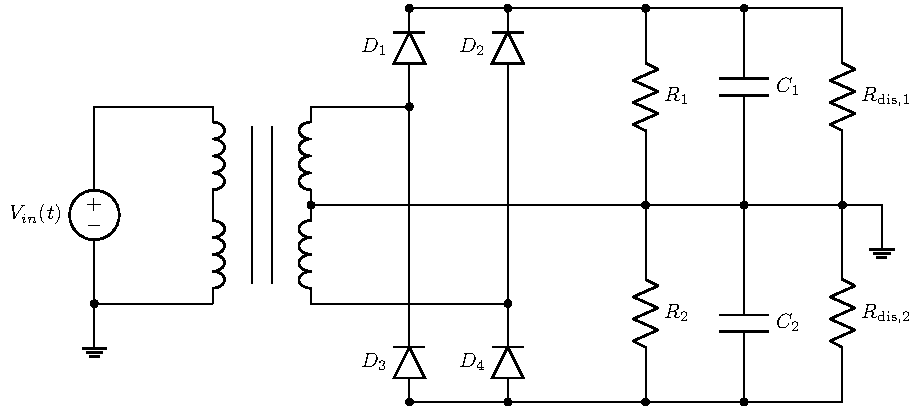
\includegraphics[width=0.75\linewidth]{TU Delft Booming Bass Project Report/figures/PowerSupply/MainPowerSupply.pdf}
    \caption{{Complete schematic of the power supply. Here, $V_{in}(t)$ represents the voltage from the wall outlet (230V, 50HZ). The primary and secondary windings are magnetically coupled, denoted by the two vertical lines indicating the magnetic core of the transformer.}}
    \label{fig:MainPowerSupplySchematic}
\end{figure}
\vspace{10pt}

The complete schematic of the power supply is shown in \sfautoref{fig:MainPowerSupplySchematic}. Each element in the schematic is clearly labeled and serves a distinct function in the design to meet the defined system requirements.
It is clear from the schematic that the power supply is dependent on multiple components and, thus, on their respective value:
\begin{itemize}
    \item \textbf{Resistors $R_{1}$ and $R_{2}$}: These resistors act and form the load of the power supply circuit, therefore simulating a real-world load. The values of the load resistors are based on the equivalent resistance of the sound-amplifying system and thus selected to ensure and to check that the output voltage remains within the desired range (e.g., 17-20 V DC) when a load current of 1.0 A is applied to the power supply circuit.
    
    \item {\textbf{Resistors} $R_{\text{dis,1}}$ \textbf{and} $R_{\text{dis,2}}$}: These resistors serve as discharge resistors, ensuring safe operation by discharging the stored energy after power supply operation. These resistors should allow the power supply to be fully discharged within 2.5 minutes after operation.
    
    \item \textbf{Capacitors $C_{1}$ and $C_{2}$}: These capacitors are essential for smoothing the rectified AC input, functioning as output filters to reduce ripple in the outgoing DC voltage at each terminal. In the power supply circuit, the AC voltage from the transformer undergoes rectification through the diodes, but fluctuations are still present in the DC output. These fluctuations are referred to as ripple. Capacitors $C_{1}$ and $C_{2}$ charge during the peaks of the DC waveform and discharge during the troughs, effectively ensuring that the DC voltage remains as stable as possible. The difference between the maximum and minimum capacitor voltage is thus called the voltage ripple. The choice of the capacitance values $C_{1}$ and $C_{2}$ and the load current determines the degree of ripple reduction and, thus, the overall stability of the output.
    
    \item \textbf{Diodes (1N5408)}: The power supply circuit diodes are responsible for rectifying the AC input into a unidirectional DC output. The actual diodes are already soldered on and differ from those chosen in the simulation process; the standard 1N4148 diodes are chosen in the LTSpice simulations for convenience.
    While they differ in primary characteristics, the 1N5408 diodes are more resilient than the 1N4148 regarding maximum repetitive peak voltage and maximum RMS voltage.
    \item \textbf{Transformer}: A center-tapped transformer to provide a dual output voltage necessary for the full wave rectification process. The transformer, therefore, provides both a positive and a negative output. The output voltage of the transformer was specified in advance and provided to the power supply subgroup.
\end{itemize}

\subsubsection{Analysis, Testing \& Measurements}
The results from simulating the circuit in LTSpice should offer valuable insight into the expected performance of the power supply, providing a theoretical understanding of its behavior.

Following the analysis of the power supply's expected performance through simulations, it is crucial to conduct real-world testing and measurements of the assembled power supply to confirm that its actual performance aligns with the predicted results. These measurements were carried out using the following:
\begin{itemize}
    \item \textbf{Oscilloscope: Tektronix TDS 2022B} An oscilloscope is necessary to conduct analysis and measurements after building the power supply to check the performance of the power supply.
    \item \textbf{Load Resistors} Large resistors are used to simulate the load of the power supply.
\end{itemize}

\subsubsection{Dimensioning Circuit Components and Elements}
Using the equation provided in the Integrated Project-1 Manual for $u_{\text{ripple}}[\%]$, the maximum voltage while maintaining a ripple percentage less than 5\% can be calculated, assuming that the average voltage after the rectifier is 19V:
\begin{flalign}\label{RippleVoltageEquation}
    u_{\text{ripple}}[\%]=\left(\frac{u_{\text{max}}-u_{\text{average}}}{u_{{average}}}\right)\cdot 100\%
\end{flalign}

Rearranging \seautoref{RippleVoltageEquation} yields the following expression for $u_{\text{max}}$:
\begin{flalign}\label{MaximumVoltageEquation}
    u_{\text{max}}=u_{\text{average}}\left(1+ \frac{u_{\text{ripple}}[\%]}{100\%}\right)
    \equnit{\si{\volt}}
\end{flalign}

Equation \ref{MaximumVoltageEquation} remains dependent on the average voltage and the ripple percentage. Therefore, the maximum voltage can be calculated for an average voltage of 19V after rectification $u_\text{average}=19V$, with $u_\text{ripple}[\%]=5\%$, which gives $u_\text{max}=19.95V$. 

\subsubsection{Smoothing Capacitors}
From the calculation, it is clear that the maximum voltage must not exceed 19.95 V to ensure that the voltage ripple remains within 5\% of the average voltage. With this constraint and limitation in place, the necessary capacitance value to keep the voltage ripple under 5\% can be determined and calculated. This calculation is based on a maximum post-rectification voltage of 19 V and during a load current of 1.0 A, using the voltage-current relationship for a capacitor:
\begin{flalign}\label{CapacitorEquation}
    I_C=C_{1,2}\frac{\mathrm{d}V_C}{\mathrm{d}t} 
    \equnit{\si{\ampere}}
\end{flalign}
For this calculation, a first-order approximation of the exponential decay of the voltage across the capacitor is applied. It is assumed that this decay follows a linear behavior, allowing it to be approximated, as shown
\begin{flalign}\label{LinearApproximation}
    \frac{\mathrm{d}V_C}{\mathrm{d}t}\approx\frac{\Delta{U_{\text{dc}}}}{\Delta{t}}
\end{flalign}
By combining Eqs. \ref{CapacitorEquation} and \ref{LinearApproximation}, the voltage-current relationship for the smoothing capacitors can be rewritten as
\begin{flalign}\label{CapacitorEquation2}
    I_C=C_{1,2}\left(\frac{\Delta U_\text{dc}}{\Delta t_{\text{dis}}}\right) 
    \equnit{\si{\ampere}}
\end{flalign}

By using \seautoref{CapacitorEquation2} and that $u_\text{max}-u_\text{average}=\frac{1}{2}\Delta U_\text{dc}$, it can be said that 
\begin{flalign}\label{CapacitanceEquation}
    C_{1,2}   &=I_C\left(\frac{1}{\left(\frac{\Delta U_{\text{dc}}}{\Delta t_\text{dis}}\right)}\right)=I\left(\frac{\Delta t_\text{dis}}{\Delta U_{\text{dc}}}\right)=I\left(\frac{\Delta t_\text{dis}}{2\left(u_{\text{max}}-u_{\text{average}}\right)}\right)
    \equnit{\si{F}}
\end{flalign}
Therefore, the required capacitance to achieve a voltage ripple below 5\% can be calculated with \seautoref{CapacitanceEquation}. Filling in for $\Delta t_\text{dis}=0.01 s$, which corresponds to half the period of 50Hz: and for the voltages $u_\text{max}=19.95V$, $u_\text{average}=19.00V$ and that $I_C=1.0A$ gives a minimum capacitance $C_{{\text{min},1,2}}=5.263$mF. 

However, it is crucial to consider that larger capacitance values could pose a significant risk due to the inrush current when the capacitor is initially charged. The rush of current occurs when the capacitor is connected to the power supply, and without sufficient series resistance, this current can spike dramatically. Larger capacitance values require more charge, leading to longer charging times and higher rush-in currents. This high current could potentially cause damage to other components if they are not rated to handle such spikes.

Additionally, larger rush-in currents can result in circuit instability, overheating of components, and thus stress on the power supply. Therefore, choosing a capacitance of $C_{{,1,2}}=6.8$mF ensures that the rush-in current remains within acceptable limits, avoiding the risks with larger capacitance values while still providing the necessary performance to meet the voltage ripple requirements. It is important to note that the calculated capacitance values apply individually to both the power supply circuit's positive and negative output terminals. Consequently, the two capacitors of equal capacitance are required to ensure proper functionality on either side of the output terminal.

\subsubsection{Discharge Resistors}\label{Discharge_Resistor_Section}
For the effective operation of the power supply and to ensure the safety of the smoothing capacitors, discharge resistors play a crucial role. Their value can be determined using the time constant of the power supply, which behaves as an RC circuit. The calculation is based on the following equation, where ${i=1,2}$ respective to each discharge resistor and each smoothing capacitor:
\begin{flalign}\label{RCCircuit}
    \tau_\text{RC}    &= R_{\text{dis,1 dis,2}}C_{1,2}
    \equnit{\si{s}}
\end{flalign}

As for the power supply circuit, the smoothing capacitors are assumed to be fully discharged after approximately 5$\tau$. Thus, it is assumed that 5$\tau\approx t_{\text{dis}}$, where $t_{\text{dis}}$ represents the discharge time. In this case, the power supply should discharge within 2.5 minutes, meaning that $t_{\text{dis,max}}=150$. Rewriting \seautoref{RCCircuit} for $R_{\text{i}}$ gives:
\begin{flalign}\label{DischargeResistor}
    R_{\text{dis,1 dis,2}}    &=\frac{\tau_\text{RC}}{C_{\text{1,2}}}=\left(\frac{{\Bigl(\frac{t_{\text{dis}}}{5}\Bigr)}}{C_{\text{1,2}}}\right)=\frac{t_{\text{dis}}}{5C_{\text{1,2}}}
    \equnit{\si{\Omega}}
\end{flalign}

Using formula \ref{DischargeResistor}, the previously calculated capacitance, $t_\text{dis}=105 s$ gives a discharge resistor of 5.7k$\Omega$. A discharge resistance of 5.7k$\Omega$ for $R_\text{dis,1}$ and $R_\text{dis,2}$ respectively ensures that the power supply fully discharges within 2.5 minutes, given a smoothing capacitance of 5.263mF at each side of the output terminals. The calculations and the corresponding \seautoref{DischargeResistor} show that reducing the discharge resistance will result in a shorter discharge time for the power supply.

The sizing of the discharge resistor influences the ripple voltage, though in some cases, its effect may be negligible. Ripple voltage arises from fluctuations in voltage as the smoothing capacitor $C_{s1,s2}$ charges and discharges between full-wave rectified peaks. The discharge resistor $R_{\text{dis}1,\text{dis}2}$ affects the discharge rate, thus influencing the ripple's extent. Higher discharge resistor values cause the smoothing capacitors to discharge more slowly, maintaining a higher voltage for a longer period between rectified peaks, resulting in a smaller ripple. With less current drawn by the load, the capacitor discharges more gradually. Conversely, lower discharge resistor values cause faster discharge, leading to a larger ripple as the voltage drops more quickly between peaks.

In some designs, the effect of the discharge resistor can be negligible if its resistance is high compared to the capacitance. In such cases, the capacitor discharges slowly, resulting in a small ripple. Therefore, the impact of the discharge resistor on the ripple may be minimal in these scenarios.

\subsection{Power Amplifier}
\label{section: design PA}

\subsubsection{Power Amplifier Circuit}
To construct the amplifier circuit, a universal power amplifier was utilized (see \sfautoref{fig: universal power-amp}). This circuit includes several components without predefined values. To determine these values, the amplifier was first divided into three distinct sections for simplification:
\begin{itemize}
    \item A passive Low-Pass Filter (p-LPF)
    \item A passive High-Pass Filter (p-HPF)
    \item An active High-Pass Filter (a-HPF)
\end{itemize}

All of these filters are first-order systems because they use a single capacitor, and their corresponding transfer functions are first-order expressions. (refer to \seautoref{eq: E}, \seautoref{eq: F} and \seautoref{eq: G}).

To ensure optimal performance of the power amplifier, the cut-off frequencies of these three filters must be spaced by a factor of 10. This separation minimizes the risk of interference between the filters and guarantees their proper functionality. The calculations of the required component values will be based on the application of the following fundamental formulas, which are detailed in this section:
\begin{flalign}
    \label{eq: V to db}
    \mathbf{H(\omega)} = 20\log\left(\frac{V_o}{V_i}\right)
    \equnit{\si{dB}}
\end{flalign}

where $V_o$ and $V_i$ are the output and input voltages, respectively. This equation allows the gain to be expressed on a dB scale. The expected gain for a non-inverting amplifier circuit is calculated as:
\begin{flalign}
    \label{eq: noninvert}
    \mathbf{G}_{\text{gain}}=\frac{V_o}{V_i}= \frac{R_f}{R_i}+1
\end{flalign}

where $R_f$ and $R_i$ are the feedback and input resistances, respectively. This equation is used to determine the amplification factor of the non-inverting amplifier circuit. To calculate the phase shift at a given frequency in the transfer function, the following equation is used:
\begin{flalign}
    \label{eq: phase}
    \phi = \arctan{\frac{\mathbf{X_{H(\omega)}}}{\mathbf{R_{H(\omega)}}}}, \qquad \mathbf{H(\omega)} = R+jX
\end{flalign}

Here, $\mathbf{X_{H({\omega})}}$ and $\mathbf{R_{H({\omega})}}$ are the imaginary and real components of the impedance, respectively. This allows the determination of the phase shift at a given frequency, which is crucial for understanding the behavior of the amplifier circuit in terms of signal timing.
Other relevant formulas will be introduced and derived in their respective sections as needed.

\subsubsection{Calculations with one circuit design}
In the course of this project, two power amplifiers were constructed- one by group B2-1 and another by group B2-2. To determine which amplifier would be integrated into the final loudspeaker system, both circuits were evaluated against the three key requirements outlined in \autoref{requirements PA} (Refer to \autoref{section: choosing a circuit} to see the evaluation). The chosen circuit is B2-1's power amplifier. For this reason, only the exact calculations for this amplifier will be shown. However, to derive the values of B2-2's amplifier, the same methods were used, only other base values were chosen.


\subsubsection{Passive High-Pass Filter (p-HPF)}
The circuit diagram of a passive high-pass filter used in the power amplifier circuit is shown in \ref{fig: pa high pass}.
\begin{figure}[H]
    \centering
    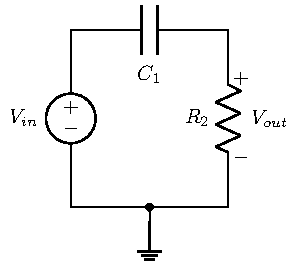
\includegraphics[width=0.3\linewidth]{TU Delft Booming Bass Project Report/figures/PowerAmplifier/circuits/HighPass filter.pdf}
    \captionsetup{justification=raggedright, labelfont=bf}
    \caption{The circuit of a passive high-pass filter.}
    \label{fig: pa high pass}
\end{figure}

The transfer function of this p-HPF circuit is derived by applying a voltage divider approach to the circuit. Initially, the conditions hold that $\mathbf{V_{out}=V_o}$:
\begin{flalign}
    \mathbf{V_o} &= \mathbf{V_i}\frac{Z_{R_2}}{Z_{R_2}+Z_{C_1}}
    \equnit{\si{V}}
\end{flalign}

This leads to the following expression for the voltage gain:
\begin{flalign}
    \mathbf{\frac{V_o}{V_i}}    &= \frac{Z_{R_2}}{Z_{R_2}+Z_{C_1}}= \frac{R_2}{R_2 + \frac{1}{sC_1}}
\end{flalign}

where $s=j\omega$. Simplifying this further and rearranging terms, the transfer function for the given p-HPF circuit is:
\begin{flalign}
\label{eq: E}
    \mathbf{E(\omega)}=\mathbf{\frac{V_o}{V_i}} = \frac{sC_1R_2}{sC_1R_2 +1 }
\end{flalign}

This transfer function confirms that the circuit behaves as a passive high-pass filter (p-HPF), as the following limits hold true for a typical RC high-pass filter circuit:
\begin{flalign}
    \lim_{\omega \rightarrow 0}\mathbf{E(\omega)}= 0\\
    \lim_{\omega \rightarrow \infty}\mathbf{E(\omega)}=1
\end{flalign}

These results are consistent with the characteristics of a high-pass filter. To determine the values of $R_a$ and $C_a$, the cut-off frequency can be derived as a function of these components. This derivation can be done by using the transfer function:
\begin{flalign}
    \mathbf{E(\omega)} = \mathbf{\frac{V_o}{V_i}} = \frac{sC_{1}R_{2}}{sC_{1}R_{2} + 1} = \frac{s}{\omega_0}\left(\frac{1}{1 + \frac{s}{\omega_0}}\right) 
\end{flalign}

Where and:
\begin{flalign}\label{eq: cutoff high}
    \omega_0 = \frac{1}{R_{2}C_{1}}
    \equnit{\si{\text{rad s^{-1}}}}
\end{flalign}

Given that $R_2=47\text{k}\Omega$ is predetermined and the desired cut-off frequency is 20Hz, the value of $C_1$ can be calculated as follows:
\begin{flalign}
    C_1 = \frac{1}{40\pi(47\cdot10^3)} = 169.3\text{nF}
    \equnit{\si{nF}}
\end{flalign}

Thus, to achieve a cut-off frequency for the passive high-pass filter of 20Hz with $R_2=47\text{k}\Omega$, the required value for $C_1$ is 169.3nF.

\subsubsection{Passive Low-Pass Filter (p-LPF)}
The circuit diagram of a passive low-pass filter used in the power amplifier circuit is shown in \sfautoref{fig: pa low pass}:
\begin{figure}[h]
    \centering
    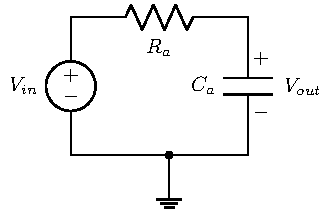
\includegraphics[width=0.3\linewidth]{TU Delft Booming Bass Project Report/figures/PowerAmplifier/circuits/LowPass filter.pdf}
    \captionsetup{justification=raggedright, labelfont=bf}
    \caption{The circuit of a passive low-pass filter .}
    \label{fig: pa low pass}
\end{figure}

The transfer function of this p-LPF circuit is derived by applying the same voltage divider approach to the circuit as with the p-HPF circuit. Initially, the conditions hold that $\mathbf{V_{out}=V_o}$:
\begin{flalign}
    \mathbf{V_o} = \mathbf{V_i}\frac{Z_{C_a}}{ Z_{R_a}+Z_{C_a}}
    \equnit{\si{V}}
\end{flalign}

This leads to the following expression for the voltage gain:
\begin{flalign}
    \mathbf{\frac{V_o}{V_i}} = \frac{Z_{C_a}}{ Z_{R_a}+Z_{C_a}}= \frac{\frac{1}{sC_a}}{R_a + \frac{1}{sC_a}}
\end{flalign}

where $s=j\omega$. Simplifying this further and rearranging terms, the transfer function for the given p-LPF circuit is:
\begin{flalign}\label{eq: F}
    \mathbf{F(\omega)} = \mathbf{\frac{V_o}{V_i}} = \frac{1}{sC_aR_a +1}
\end{flalign}

This transfer function confirms that the circuit behaves as a passive low-pass filter (p-LPF), as the following limits hold true for a typical RC low-pass filter circuit:
\begin{flalign}
    \lim_{\omega \rightarrow 0}\mathbf{F(\omega)}= 1\\
    \lim_{\omega \rightarrow \infty}\mathbf{F(\omega)}=0
\end{flalign}

These results are consistent with the characteristics of a low-pass filter. To determine the values of $R_a$ and $C_a$, the cut-off frequency can be derived as a function of these components. This derivation can be done by using \seautoref{eq: F}, thus giving us a similar transfer function as \seautoref{eq: cutoff high}:
\begin{flalign}
    \mathbf{F(\omega)} = \frac{1}{sC_{a}R_{a}+1} = \frac{1}{\left(\frac{s}{\omega_0} + 1\right)}
\end{flalign}

where $s=j\omega$, and: 
\begin{flalign}\label{eq: cutoff low}
    \omega_0 = \frac{1}{R_{a}C_{a}}
    \equnit{\si{\text{rad s^{-1}}}}
\end{flalign}

The value of $R_a$ was selected as 1k$\Omega$ due to its simplicity for calculations. Given a cut-off frequency of 40kHz for the p-LPF, and $R_a=1\text{k}\Omega$, the corresponding value for $C_a$ is calculates as:
\begin{flalign}
    C_a = \frac{1}{80\text{k}\pi\left(1.0\cdot 10^{3}\right)} = 3.98\text{nF}
    \equnit{\si{nF}}
\end{flalign}

Thus, to achieve a cut-off frequency for the passive low-pass filter (p-LPF) of 40kHz with $R_a=1\text{k}\Omega$, the required value for $C_a$ is 3.98nF.


\subsubsection{Active High-Pass Filter (a-HPF)}
The circuit diagram of an active high-pass filter is shown in \sfautoref{fig: pa active high pass}:
\begin{figure}[H]
    \centering
    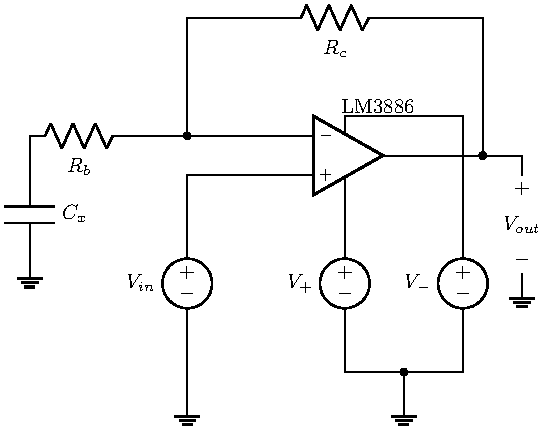
\includegraphics[width=0.4\linewidth]{TU Delft Booming Bass Project Report/figures/PowerAmplifier/circuits/active_high_pass.pdf}
    \captionsetup{justification=raggedright, labelfont=bf}
    \caption{The circuit of an active high-pass filter (a-HPF).}
    \label{fig: pa active high pass}
\end{figure}

The final filter is an active high-pass filter. In this filter, $C_x$ serves a crucial role in blocking any DC voltage from reaching the operational amplifier (op-amp). This DC voltage could originate from the input signal or from an offset voltage between the two input terminals of the op-amp, which results from its non-ideal characteristics. By blocking the DC component, this function prevents any residual DC voltage from being amplified, thus protecting the loudspeaker from potential damage.

As specified in the IP-1 manual \cite{IP-manual}, the op-amp used in this power amplifier circuit is the 'LM3886 Operational Amplifier'. The LM3886 offers several beneficial properties, mentioned in \cite{IP-manual}:

\begin{enumerate}
    \item A high input resistance of 200k$\Omega$. 
    \item A low output resistance of 10$\Omega$. 
    \item A large open-loop voltage gain of $10^5$.
\end{enumerate}

These characteristics are relatively close to ideal, allowing calculations involving the LM3886 to be made under the assumption that it behaves as an ideal op-amp.

The transfer function for this active high-pass filter can be derived using nodal analysis at the input terminals of the op-amp:
\begin{flalign}
    \mathbf{V_{in} = V_{-}}
    \equnit{\si{V}}
\end{flalign}
where the input voltage $V_{in}$ equals the negative op-amp voltage, denoted by $V_{-}$. Nodal analysis on the active high-pass filter circuit gives:
\begin{flalign}
    \frac{V_i}{Z_{R_b}+Z_{C_x}} = \frac{V_{o}-V_{i}}{Z_{R_c}}\\
    \left(\frac{1}{R_b + Z_{C_x}} + \frac{1}{R_C}\right)V_i = \frac{V_o}{R_c}
\end{flalign}

Simplifying this further and rearranging terms, the transfer function for the given a-HPF circuit is:
\begin{flalign}
    \label{eq: G}
    \mathbf{G(\omega)} = \mathbf{\frac{V_o}{V_i}} = \frac{R_C}{R_b + \frac{1}{s C_x}}+1
\end{flalign}

The behavior of an a-HPF can again be shown by $\omega$ approaching 0 and $\infty$:

\begin{flalign}
    \lim_{\omega \rightarrow 0}\mathbf{G(\omega)}= 1\\
    \lim_{\omega \rightarrow \infty}\mathbf{G(\omega)}=\frac{R_c}{R_b} + 1
\end{flalign}

At very low frequencies, the gain goes to 1, while at very high frequencies, $C_x$ acts as a short circuit, allowing the a-HPF filter to achieve its maximum gain. This behavior is characteristic to an active high-pass filter. 


Since this circuit also functions as a high-pass filter, \seautoref{eq: cutoff high} can be applied again, substituting $R_2$ and $C_1$ with $R_b$ and $C_x$ respectively to calculate the relevant values. The role of $C_x$ is to prevent amplification of the DC offset generated within the op-amp. As the frequency approaches zero, the impedance of $C_x$ increases, causing it to behave like an open circuit and turning the amplifier into a voltage follower. Given that this frequency must be an order of 10 lower than the low-pass filter cut-off frequency, a frequency of 2Hz was selected. Using $R_b=80\text{k}\Omega$ (chosen for the ease of obtaining a simple value for $C_x$) and $f=2\text{Hz}$, the value of $C_x$ can be calculated as follows: 
\begin{flalign}
    C_x = \frac{1}{4\pi(80\cdot10^{3})} = 1 \mathrm{\mu F}
    \equnit{\si{\mu{F}}}
\end{flalign}


\subsubsection{Calculating $\mathbf{R_c}$}

To calculate $R_c$, capacitor $C_x$ can be considered a short circuit, as the cut-off frequency is 2Hz, which is a decade lower than the frequencies expected to pass through the circuit. In this scenario, the circuit behaves as a standard non-inverting amplifier. Therefore, \seautoref{eq: noninvert} can be applied, where $R_f$ and $R_i$ correspond to $R_c$ and $R_b$, respectively, assuming the op-amp operates ideally. Using $R_b=80\text{k}\Omega$ and a voltage gain of $\mathbf{V_o}$/$\mathbf{Vi}$=25, the value of $R_c$ can be determined as follows:

\begin{flalign}
   \frac{V_o}{V_i}  &= \frac{R_c}{R_b}+ 1 \Rightarrow R_c=R_b(25-1)=24R_b\\
    R_c &=1.92\text{M}\Omega
\end{flalign}

To verify this ratio, nodal analysis was performed on the active high-pass filter circuit, assuming non-ideal conditions. For simplification, a resistor value of 1k$\Omega$ was used for $R_b$ instead of 80k$\Omega$, which aided in streamlining the subsequent calculations (refer to \autoref{calculation of Rc} for the complete calculation). 

To further validate that the entire power amplifier circuit operates as a band-pass filter, the transfer function of the full circuit was derived. The transfer function in  \seautoref{eq: E}, \seautoref{eq: F}, and \seautoref{eq: G} were multiplied together to obtain the total transfer function (see \autoref{total transfer} for the complete calculation and derivation). The resulting response is as follows:

% Just to confirm that the complete power amplifier circuit behaves as a band-pass filter (BPF), this is again done with a transfer function. To obtain the complete transfer function of the circuit,  \seautoref{eq: E}, \seautoref{eq: F}, and \seautoref{eq: G} have to be multiplied by each other (for the full calculation, see \autoref{total transfer}). This response ended up being:  
\begin{flalign}\label{eq: total transfer}
    \mathbf{H(\omega)} = \frac{s^2 (af+ k) + s a }{e \big(sf + 1 \big)}
\end{flalign}

where $a=R_{2}C_{1}$, $b=R_{a}C_{a}$, $d=ab$, $f=R_{b}C_{x}$, $k=aR_{c}C_{x}$, and $e=s^{2}d+sa+sb+1$.
This transfer function confirms the band-pass nature of the circuit, as the following limits hold true:
\begin{flalign}
    \lim_{\omega \rightarrow 0}\mathbf{H(\omega)}= 0\\
    \lim_{\omega \rightarrow \infty}\mathbf{H(\omega)}=0
\end{flalign}

This behavior of the transfer function $\mathbf{H(\omega)}=0$ is immediately apparent when $\omega$ goes to infinity and can be explained by the structure of the transfer function; the numerator is a second-order equation, while the denominator is a third-order equation. As $\omega$ approaches infinity, the denominator increases at a faster rate than the numerator, causing the entire equation to approach zero (see \seautoref{eq: third order}).

\begin{figure}[H]
    \centering
    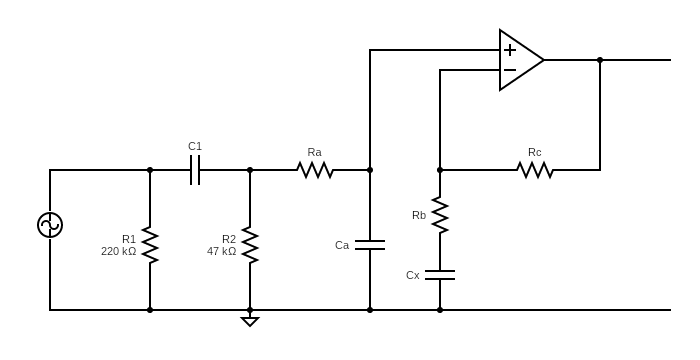
\includegraphics[width=0.7\linewidth]{TU Delft Booming Bass Project Report/figures/PowerAmplifier/circuits/circuit.png}
    \captionsetup{justification=raggedright, labelfont=bf}
    \caption{A universal circuit for a power amplifier.}
    \label{fig: universal power-amp}
\end{figure}

In the lab, components are not available at every possible value. As a result, the ideal values calculated for the power amplifier circuit could not be directly implemented; instead, they were replaced with components whose values were as close as possible to the initially calculated values. The calculated ideal values and the final chosen values are listed in \stautoref{tab:B2-1 ideal values}. Since the power amplifier used in the final system is from group B2-1, all calculations in this section are based on the data from B2-1's power amplifier. Data obtained by group B2-2 are presented in \stautoref{tab:B2-1 ideal values}.


\begin{table}[H]
    \centering
    \caption{B2 Summary of calculated and chosen (Resistance $R_N$, capacitance $C_N$, and cut-off frequency $f_{\text{cut-off}}$) values for the p-HPF, p-LPF, a-HPF, with $D_{\text{diff}}[\%]$ representing the deviation between the calculated and used values.}
    \resizebox{\textwidth}{!}{
    \begin{tabular}{c @{\hspace{12pt}} *4{c} S @{\hspace{12pt}} *4{c} S @{\hspace{12pt}}}
        \toprule
        \multicolumn{9}{c}{\textbf{B2 Filter Component Parameters}} \\
        \cmidrule(lr){1-9}
        & & \multicolumn{3}{c}{\textbf{B2-1 Component Values}} & & \multicolumn{3}{c}{\textbf{B2-2 Component Values}} \\
        \cmidrule(lr){3-5} \cmidrule(lr){7-9}
        & Parameter & Calc. Value & Used Value & $D_{\text{diff}}$ [\%] & & Calc. Value & Used Value & $D_{\text{diff}}$ [\%] \\
        \midrule
        p-HPF & $R_2$ [$\Omega$] & 47k$\Omega$ & 47k$\Omega$ & 0.00\% & & 47k$\Omega$ & 47k$\Omega$ & 0.00\% \\
         & $C_1$ [F] & 169.3nF & 166.5nF & -1.65\% & & 169.3nF & 220nF & 29.94\% \vspace{4pt} \\
         & $f_\text{cut-off}$ [Hz] & 20Hz & 20Hz & 0.00\% & & 13Hz & 20Hz & 53.85\% \vspace{10pt} \\
        p-LPF & $R_a$ [$\Omega$] & 1k$\Omega$ & 987$\Omega$ & -1.3\% & & 12$\Omega$ & 680$\Omega$ & 5567\% \\
         & $C_a$ [F] & 3.98nF & 4.05nF & -1.73\% & & 330nF & 6.8nF & -97.96\% \vspace{4pt}\\
         & $f_\text{cut-off}$ [Hz] & 40kHz & 40kHz & 0.00\% & & +100kHz & 34kHz & - \vspace{10pt}\\
        a-HPF & $R_c$ [$\Omega$] & 1.92M$\Omega$ & 1.92M$\Omega$ & 0.00\% & & 1.92M$\Omega$ & 1.92M$\Omega$ & 0.00\% \\
        & $R_b$ [$\Omega$] & 80k$\Omega$ & 81.8k$\Omega$ & 2.25\% & & 2kM$\Omega$ & 2k$\Omega$ & 0.00\% \\
         & $C_x$ [F] & 1$\mu$F & 968nF & -1.4\% & & 8.3$\mu$F & 8.2$\mu$F & -1.20\% \vspace{4pt} \\
         & $f_\text{cut-off}$ [Hz] & 2Hz & 2Hz & 0.00\% & & 9.6Hz & 9.6Hz & 0.00\% \\
        \bottomrule
    \end{tabular}
    }
    \captionsetup{justification=raggedright, labelfont=bf}
    
    \label{tab:B2-1 ideal values}
\end{table}

\subsection{Filters - Loudspeaker Circuit Models}
\subsubsection{Model at Resonant Frequency}
The behavior of the speakers can be represented by an equivalent circuit comprising resistors, capacitors, and inductors. The capacitors and inductors model the speaker's frequency-dependent characteristics. At certain frequencies, the speaker exhibits predominantly higher resistive behavior, primarily influenced by the natural resonant frequency of the speaker's cone. The circuit model consists of five elements arranged as shown in \sfautoref{fig:impedance_model1}. Here, $R_e$ represents the impedance at DC conditions, $L_e$ models the inductance of the voice coil, and the parallel RLC branch represents the mechanical properties of the cone. In this parallel branch, $R_p$ corresponds to frictional losses, $L_p$ models the mass of the cone, and $C_p$ represents its spring-like behavior \cite{johnshopkins_rlc}.
\begin{figure}[H]
    \centering
    \captionsetup{justification=raggedright, labelfont=bf}
    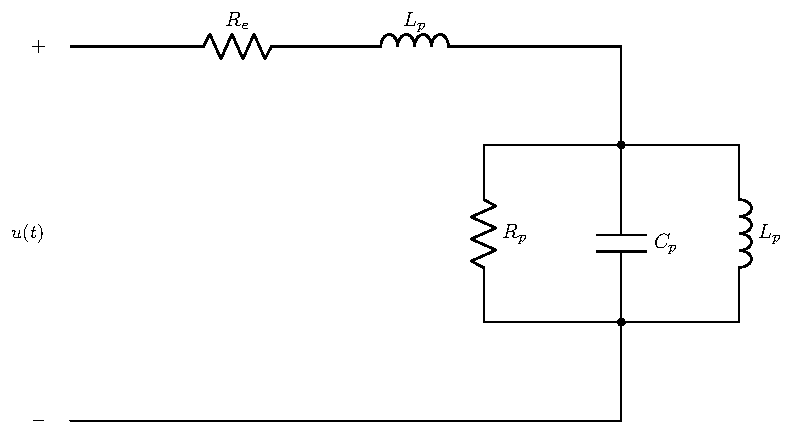
\includegraphics[width=0.6\linewidth]{figures/FilterGroup/ImpedanceModel1.pdf}
    \caption{Impedance model of the loudspeakers, depicting the equivalent circuit configuration used to represent the speaker's electrical ($R_e$, $L_e$) and mechanical properties ($R_p$, $C_p$, $L_p$ )\cite{IP-manual}.}
    \label{fig:impedance_model1}  
\end{figure}

\subsubsection{Model above Resonant Frequency}
At frequencies above and significantly higher than the cone's resonant frequency, the equivalent circuit can be further simplified. The total impedance of the circuit could be calculated using \seautoref{eq:total impedance}. For $\omega \gg \omega_o$, where $\omega_o$ is the resonant frequency of the circuit, the parallel components $R_p, C_p$ and $L_p$ can be disregarded due to their diminished influence on the overall impedance. To justify this simplification, the analysis should employ a normalized angular frequency $\omega'$ defined as follows:
\begin{flalign}
    \label{eq:normalize frequency}
    \omega' = \frac{\omega}{\omega_o}
%    \equnit{\si{\text{rad s^{-1}}}}  Heeft geen units, want normalized
\end{flalign}
The total impedance of the loudspeaker model is given by
\begin{flalign}
    \label{eq:total impedance}
    Z_{tot} = R_e + j\omega L_e + \frac{1}{\frac{1}{R_p}+j\omega C_p+\frac{1}{j\omega L_p}}
    \equnit{\si{\Omega}}
\end{flalign}

By applying \seautoref{eq:normalize frequency} and substituting it into \seautoref{eq:total impedance}, a revised expression for the total impedance, $Z_{tot}$, is obtained, as presented in \seautoref{eq:normalized impedance}:
\begin{equation}
    \label{eq:normalized impedance}
    Z_{tot} = R_e + j\frac{\omega'}{\sqrt{L_pC_p}}L_e + \frac{1}{\frac{1}{R_p}+j\sqrt{\frac{C_p}{L_p}}\left(\omega'-\frac{1}{\omega'}\right)}
    \equnit{\si{\Omega}}
\end{equation}

The angular frequency $\omega$ can be expressed as $\omega'\omega_o$, where $\omega'$ is the normalized angular frequency, and $\omega_o$ is the resonant frequency. Substituting the expression for $\omega_o$ from Eq.\ref{eq:resonant frequency appA}\cite{IP-manual}, the final expression for $\omega$ is derived and presented in \seautoref{eq:final omega appA}.
\begin{flalign}
    \label{eq:resonant frequency appA}
    \omega_o = \frac{1}{\sqrt{L_pC_p}}
    \equnit{\si{\text{rad s^{-1}}}}
\end{flalign}
\begin{flalign}
    \label{eq:final omega appA}
    \omega = \frac{\omega'}{\sqrt{L_pC_p}}
    \equnit{\si{\text{rad s^{-1}}}}
\end{flalign}

In the following section, $Z_{par}$ will be defined as the impedance of the parallel RLC portion of the equivalent circuit. Its expression is provided in \seautoref{eq:parallel impedance appA}:
\begin{flalign}
    \label{eq:parallel impedance appA}
    Z_{par} = \frac{1}{\frac{1}{R_p}+j\omega C_p+\frac{1}{j\omega L_p}}
    \equnit{\si{\Omega}}
\end{flalign}


To examine the behavior of $Z_{par}$ when $\omega \gg \omega_o$, we can investigate the impedance as $\omega'\gg 1$. To do this first, we first need to rewrite the equation in terms of $\omega'$:
\begin{flalign}
\label{eq:capacitive_impedance appA}
    j\omega C_p = j\omega'\sqrt{\frac{c_p}{L_p}}
    \equnit{\si{\Omega^{-1}}}
\end{flalign}

\begin{flalign}
\label{eq:inductive_impedance appA}
    \frac{1}{j\omega L_p} = -j\frac{1}{\omega'}\sqrt{\frac{C_p}{L_p}}
    \equnit{\si{\Omega^{-1}}}
\end{flalign}

Substituting Eq~\ref{eq:capacitive_impedance appA} and Eq~\ref{eq:inductive_impedance appA} into Eq~\ref{eq:parallel impedance appA} will result in Eq~\ref{eq:normalized impedance appA}.

\begin{flalign}
    \label{eq:normalized impedance appA}
    Z_{par} = \frac{1}{\frac{1}{R_p}+j\sqrt{\frac{C_p}{L_p}}(\omega'-\frac{1}{\omega'})}
    \equnit{\si{\Omega}}
\end{flalign}

It can now be observed that if $\omega'\gg1$, then $Z_{par} \ll 1$. Since $Z_{tot} = R_e + j\omega L_p + Z_{par}$, it follows that for $\omega \gg \omega_o$, the total impedance can be approximated as $Z_{tot} \approx R_e + j\omega L_p$.

The revised expression for $Z_{tot}$ corresponds to an equivalent circuit consisting of an inductor and a resistor, as shown in Fig \ref{fig:impedance_model2}. If the operating frequencies of the speaker are all significantly higher than the resonant frequency, utilizing this simplified model becomes more practical for analysis and design purposes.
\begin{figure}[H]
    \centering
    \captionsetup{justification=raggedright, labelfont=bf}
    \includegraphics[width=0.5\linewidth]{figures/FilterGroup/impedance_model2_speaker.jpg}
    \caption{Impedance model for frequencies above the resonant frequency, illustrating the simplified equivalent circuit consisting of an inductor $L_e$ and the resistor $R_e$ \cite{IP-manual}.}
    \label{fig:impedance_model2}
\end{figure}

\subsubsection{Calculate Model Parameters}
The determination of the five unknown parameters requires solving a set of five equations. By analyzing the circuit and its impedance, the necessary equations for parameter estimation can be derived. The measured impedance data is presented in Fig \ref{fig:abs_speakers}. Detailed derivations of these equations are provided in the IP-manual \cite{IP-manual}.
\begin{flalign}
    \label{eq:Re_model}
    R_e = \left. |Z| \right._{\omega=0}
    \equnit{\si{\Omega}}
\end{flalign}

Where $R_e$ represents the equivalent resistance of the circuit under DC conditions, corresponding to the impedance when the frequency is zero ($\omega=0$). Similarly, the parallel resistance $R_p$ is derived by subtracting $R_e$ from the magnitude of the total impedance $|Z|$ at the resonant angular frequency denoted by $\omega= \omega_o$, as given in \seautoref{eq:Rp_model}:
\begin{flalign}
    \label{eq:Rp_model}
    R_p = \left. |Z| \right._{\omega=\omega_o} - R_e
    \equnit{\si{\Omega}}
\end{flalign}

Where $R_p$ accounts for the frictional losses in the mechanical behavior of the speaker at resonance. The capacitance $C_p$, representing the spring behavior of the speaker cone, is related to $R_p$ by \seautoref{eq:Cp_model}:
\begin{flalign}
    \label{eq:Cp_model}
    C_p = \frac{1}{R_pB}
    \equnit{\si{F}}
\end{flalign}

Where B characterizes the bandwidth of the speaker's cone, the inductance $L_p$, representing the mass of the speaker cone, is related to $C_p$ and the resonant angular frequency $\omega_o$ by \seautoref{eq:Cp_model}. 
The inductance $L_e$, which models the voice coil, can be derived from the impedance at high frequencies ($\omega \gg \omega_o$) using Eq \ref{eq:Le_model}:
\begin{flalign}
    \label{eq:Lp_model}
    L_p = \frac{1}{C_p\omega_o^2}
    \equnit{\si{H}}
\end{flalign}
\begin{flalign}
    \label{eq:Le_model}
    L_e = \frac{\sqrt{(|Z|_{\omega \gg \omega_o})^2-R_e^2}}{\omega}
    \equnit{\si{H}}
\end{flalign}

The next step involves solving the equations for the different speakers and simulating the models to compare their responses with the actual measured data. Tab.\ref{tab:speaker_components} presents the calculated component values.
\begin{figure}[H]
    \centering
    \begin{minipage}{0.5\textwidth}
        \centering
        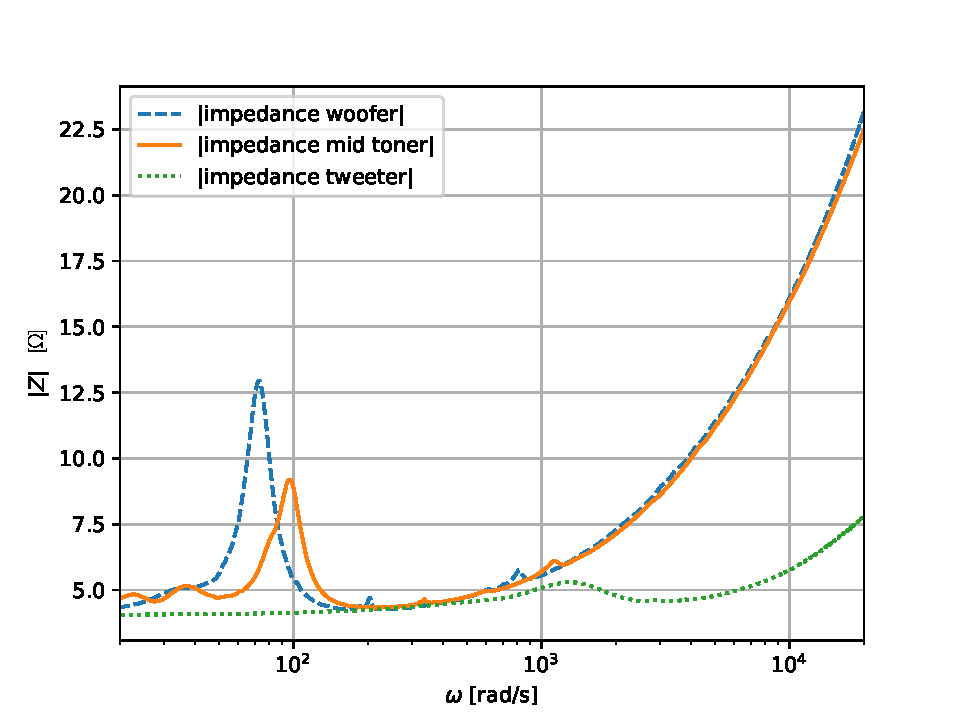
\includegraphics[width=\linewidth]{TU Delft Booming Bass Project Report/figures/FilterGroup/abs_impedance_speakers (2).pdf}
        \captionsetup{justification=raggedright, labelfont=bf}
        \caption{Absolute value of the speaker impedance.}
        \label{fig:abs_speakers}
    \end{minipage}\hfill
    \begin{minipage}{0.5\textwidth}
        \centering
        \captionsetup{justification=raggedright, labelfont=bf}
        \caption{Component Values for the woofer, tweeter, and mid-toner, showing each component's resistance, inductance, and capacitance values. The table highlights the different characteristics of the components used in the speaker system.}
        \begin{threeparttable}
          \centering
          \begin{tabular}{c @{\hspace{12pt}} *4{c} S @{\hspace{12pt}}}
            \toprule
            \multicolumn{5}{c}{\textbf{Speaker Component Values}} \\
            \cmidrule(lr){1-5}
            & & \multicolumn{3}{c}{\textbf{Component Values}} \\
            \cmidrule(lr){3-5}
            & Component & Woofer & Tweeter & Midtoner \\
            \midrule
            1 & $R_e$ [$\Omega$] & 4.03 & 4.14 & 4.06 \\
            2 & $L_e$ [mH] & 0.182 & 0.247 & 0.053 \\
            3 & $R_p$ [$\Omega$] & 8.93 & 5.05 & 1.24 \\
            4 & $C_p$ [mF] & 1.31 & 1.75 & 0.14 \\
            5 & $L_p$ [mH] & 3.66 & 1.67 & 0.11 \\
            \bottomrule
          \end{tabular}
        \end{threeparttable}
        
        \label{tab:speaker_components}
    \end{minipage}
\end{figure}

\subsubsection{Model Transfer Function}
A transfer function is the ratio between an output value and an input value of a signal into and out of a system. It can be constructed with the use of \seautoref{eq:transfer_function}, where {$\mathbf{Y(\omega)}$} is the output signal and $\mathbf{X(\omega)}$ is the input signal. It can therefore be used to characterize a system \cite{IP-manual} and is a way to examine the behavior of the system at every frequency.
%The transfer function $\mathbf{H(\omega)}$ of the system describes the behaviour of the system. It relates the input to the output of the system with the use of \seautoref{eq:transfer_function}, where {$\mathbf{Y(\omega)}$} is the output signal and $\mathbf{X(\omega)}$ is the input signal. 
In the case of the loudspeaker analysis, the input signal is the voltage $\mathbf{V(\omega)}$, and the output signal is $\mathbf{I(\omega)}$. The transfer function will represent the input impedance $\mathbf{Z(\omega)}$ of the entire circuit. 
\begin{flalign}
    \label{eq:transfer_function}
    \mathbf{Y(\omega)} = \mathbf{H(\omega)X(\omega)}
\end{flalign}

In our case, the transfer function is the system impedance. So, finding the transfer function is a matter of finding the equivalent impedance using the basic calculation rules for parallel and series circuits. First, we transform the circuit into the phasor domain as seen in \sfautoref{fig:/model_phasor}. The total impedance is calculated with \seautoref{eq:total_impedance} where $Z_{par}$ resembles the impedance of the three parallel components, and its value is calculated with \seautoref{eq:parallel_impedance}. combining the two equations results in \seautoref{eq:final_impedance}, which is the total transfer function.
\begin{flalign}
    \label{eq:total_impedance}
    Z(\omega) = R_e + j\omega L_e + Z_{par}
    \equnit{\si{\Omega}} 
\end{flalign}
\begin{flalign}
    \label{eq:parallel_impedance}
    Z_{par}(\omega) = \frac{L_pR_p\omega}{jC_pR_pL_p\omega^2+L_p\omega-jR_p}
    \equnit{\si{\Omega}} 
\end{flalign}
\begin{flalign}
    \label{eq:final_impedance}
    Z(\omega) = \frac{L_pR_p\omega + (L_e\omega+R_e)(jC_pR_pL_p\omega^2+L_p\omega-jR_p)}{jC_pR_pL_p\omega^2+L_p\omega-jR_p}
    \equnit{\si{\Omega}} 
\end{flalign}
\begin{figure}[H]
    \centering
    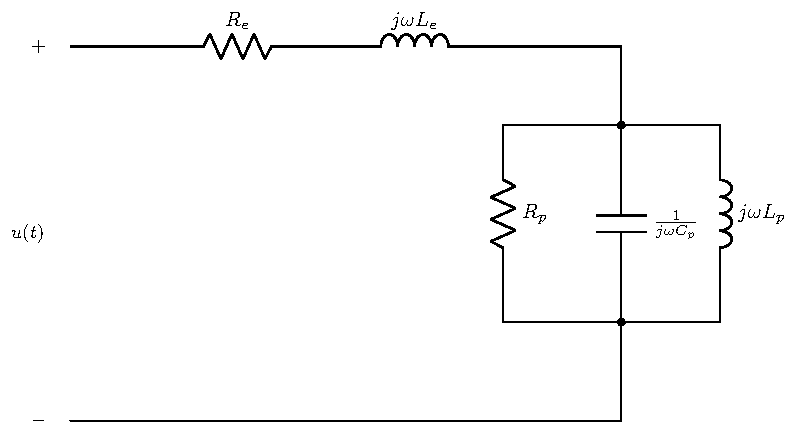
\includegraphics[width=0.5\linewidth]{TU Delft Booming Bass Project Report/figures/FilterGroup/impedance_model_phasor.pdf}
    \captionsetup{justification=raggedright, labelfont=bf}
    \caption{Equivalent model of the circuit in phasor domain.}
    \label{fig:/model_phasor}
\end{figure}

\section{Filters - Filter design}
\subsubsection{Order of the Filters}
The initial requirement is choosing the order of the filter. This will be the base of the entire filter, as it decides what type of components the filter uses. The order of the filter changes the rate at which its amplitude responds around its cut-off frequencies. The transfer function of a first-order filter will decline by 20 decibels per decade (20dB/decade), whereas a second-order filter's transfer function will decline by 40 decibels per decade (40dB/decade). 

The significance of the greater decline is that the filter will act closer to an ideal filter, which would, therefore, make it fit closer to the models made for these filters. This is because, at the cut-off frequency, the filters' amplitude response will decrease to the half-power amplitude quicker with a steeper decline in the amplitude. At and after the half-power amplitude, it can be approximated that the frequencies have a negligible impact on the speaker cone, as their power is not enough to significantly amplify the sound. Therefore, it was reasoned that a second-order filter was in the best interest of the amplifier, as it would allow the filters to be bound more to the frequencies assigned to them and have an insignificant impact outside this range. 

\subsubsection{Zobel Network}
As shown in \sfautoref{fig:/model vs measured impedance}, the impedance of the speaker increases at higher frequencies, which can lead to an increase in voltage across the loudspeaker. Consequently, this results in an increase in the difference of sound pressure produced by the speaker, as referenced in \cite{IP-manual}.

There are two potential solutions to mitigate this issue and its undesirable effect on the filters. The first is to account for the frequency-dependent impedance of the speaker in the design. The second option is to add a Zobel network parallel to the filter. A Zobel network consists of components connected in parallel with the speaker element to ensure that the combined impedance is purely resistive (In the real domain). This results in a constant impedance, simplifying the calculation process.

However, designing a Zobel network presents challenges, as it requires simulating the network to determine the optimal component values. Even once this is achieved, the limitations of available components in the lab may prevent the Zobel network from eliminating the reactance of the loudspeaker (the complex part of the impedance). It is more likely to only reduce the frequency dependence of the impedance. Based on these considerations, the group decided that implementing a Zobel network was not appropriate for this project, and therefore it was not used.

\subsubsection{Cut-off Frequency Calculations}
The cut-off frequencies are defined as the points where the transfer functions gain reaches $\sqrt{2}/2$, commonly referred to as the -3dB frequency. For low-pass filters, frequencies above this point have minimal and, thus, a negligible effect on the output. In the case of a band-pass filter, there are two cut-off frequencies; frequencies outside this range, both before the first and after the second cut-off, do not significantly affect the output. Lastly, for high-pass filters, the frequencies before the cut-off frequencies do not have a significant effect on the output.

Selecting the appropriate cut-off frequencies is crucial, as the primary goal of the project is to achieve the flattest possible acoustic response. The cut-off frequencies determine the optimal frequency ranges for each speaker, ensuring that each cone operates within its optimal range. Tweeters perform best at high frequencies (2kHz - 20kHz), bass at low frequencies (\~40Hz - 400Hz), and mid-toners in the middle range. Frequencies outside this range can either degrade the sound quality or potentially damage the speaker cone. Therefore, it is essential to carefully select these cut-off frequencies.
The optimal cut-off frequencies were determined by overlaying the acoustic responses of each speaker using Python, as shown in \sfautoref{fig: Cutoff frequencies}. By visual inspection and understanding each speaker's ideal frequency range, the cut-off frequencies were selected. The approach involved identifying the frequencies where each speaker began to show instability and where the next speaker could take over smoothly in their frequency range. This careful selection, accounting for constructive and destructive interference between sound waves, allowed for the flattest possible overall response.

The final choice for the low-pass filter's cut-off frequency was 200Hz, as it produced the flattest overall acoustic response, as seen in \sfautoref{fig: Cutoff frequencies}. For the high-pass filter, the cut-off frequency was set at 1250Hz to provide a smooth transition between the high-pass and band-pass filters. However, it is important to note that at 900Hz in \sfautoref{fig: Cutoff frequencies}, there is a noticeable dip in the mid-toner's power response. This dip affects the overall response before the cut-off frequency. Despite efforts to select the optimal cut-off frequencies, this dip remained a factor to be cautious of in the design process.
\begin{figure}[H]
    \centering
    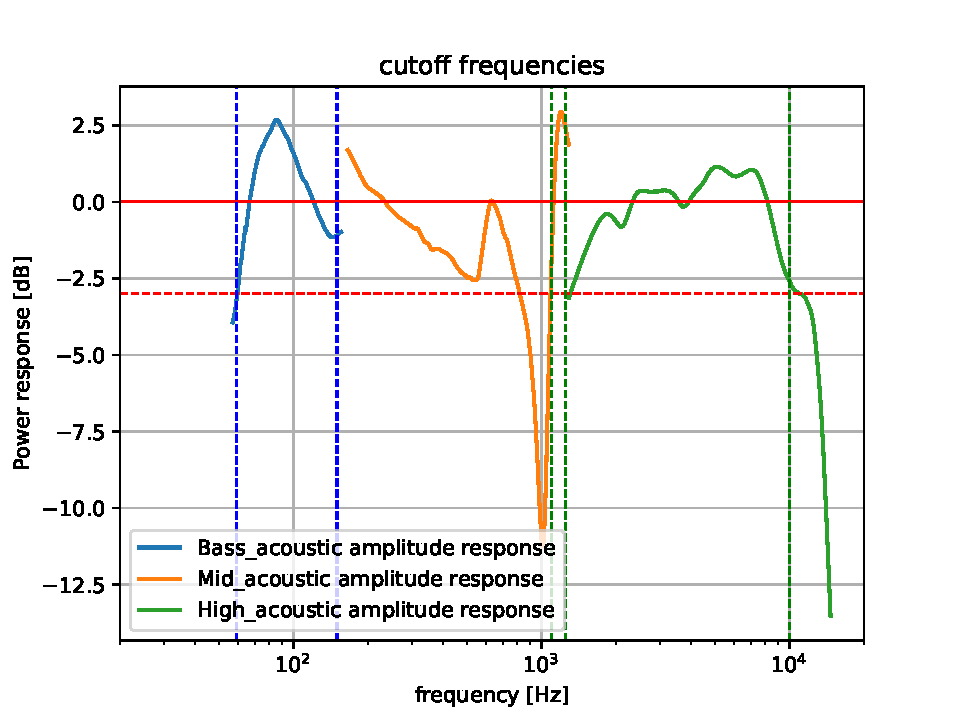
\includegraphics[width=0.65\linewidth]{TU Delft Booming Bass Project Report/figures/FilterGroup/chosenvalues.pdf}
    \captionsetup{justification=raggedright, labelfont=bf}
    \caption{Amplitude responses of the various filters plotted to aid in selecting the initial cut-off frequencies, denoted by $\omega_c$, for optimal frequency separation.}
    \label{fig: Cutoff frequencies}
\end{figure}

\subsubsection{Filters Transfer Function}
The transfer functions of the filters describe the relationship between the input voltage and the output voltage of the filter. By using \seautoref{eq:transfer_function}, a relevant transfer function can be derived for each filter, enabling the analysis of their frequency responses. This approach is invaluable in the design process, as it allows for a comprehensive examination of the filter's behavior across a wide range of frequencies. Such an analysis helps ensure that the filter performs as expected and meets the desired specifications, guiding the optimization of filter parameters.

The High-Pass Filter (HPF) is composed of components shown in \sfautoref{fig:HighPassFilter}. In this configuration, the loudspeaker impedance, denoted as $Z_l$, is modeled as a single component. By applying nodal analysis to the high-pass filter circuit in \sfautoref{fig:HighPassFilter}, the transfer function, as expressed in \seautoref{High pass filter Transfer function}, can be derived. This transfer function characterizes the relationship between the input and output voltages of the filter, facilitating the analysis of the filter's behavior across different frequencies.
\begin{flalign}
    \label{High pass filter Transfer function}
    \mathbf{H_{HPF}(\omega)} = \frac{C_HL_HZ_l\omega^2}{C_HL_HZ_l\omega^2-j\omega L_{H}-Z_l}
\end{flalign}

where $C_H$ and $L_H$ are the capacitance and inductance of the High-Pass Filter (LPF), denoted by subscript $H$, respectively.
Furthermore, the Low-Pass Filter in Fig \ref{fig:LowPassFilter} was analyzed with nodal analysis, which resulted in the transfer function in Eq \ref{Low pass filter Transfer function}
\begin{flalign}
    \label{Low pass filter Transfer function}
    \mathbf{H_{LPF}(\omega)} = \frac{-Z_l}{L_LC_LZ_l\omega^2-j\omega L_{L}-Z_l}
\end{flalign}

where $C_L$ and $L_L$ are the capacitance and inductance of the Low-Pass Filter (LPF), denoted by subscript $L$, respectively.
Moreover, the band-pass filter in Fig \ref{fig:BandPassFilter} was examined with nodal analysis, where the transfer function in Eq \ref{Band pass filter Transfer function} was found.
\begin{flalign}
    \label{Band pass filter Transfer function}
    \mathbf{H_{BPF}(\omega)} = \frac{jC_HL_HZ_l\omega^2}{-jC_HC_LL_HL_LZ_l\omega^4-C_HL_HL_L\omega^3+jZ_l\omega^2(C_HL_H+C_LL_H+C_LL_L)+(L_H+L_L)\omega-jZ_l}
\end{flalign}
\begin{figure}[H]
    \centering
    \begin{minipage}{0.29\textwidth}
        \centering
        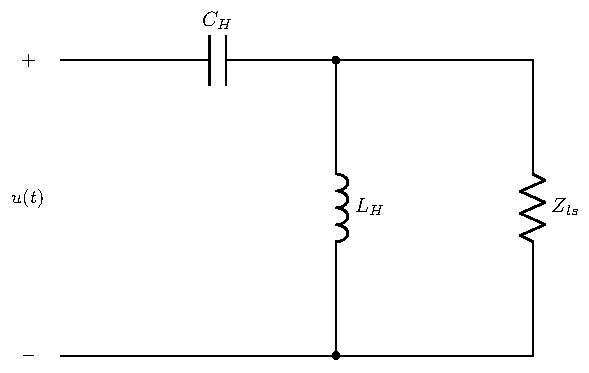
\includegraphics[width=\linewidth]{TU Delft Booming Bass Project Report/figures/FilterGroup/High pass filter schematic.pdf}
        \captionsetup{justification=centering}
        \subcaption{High-pass filter schematic.}
        \label{fig:HighPassFilter}
    \end{minipage}%
    \hfill
    \begin{minipage}{0.29\textwidth}
        \centering
        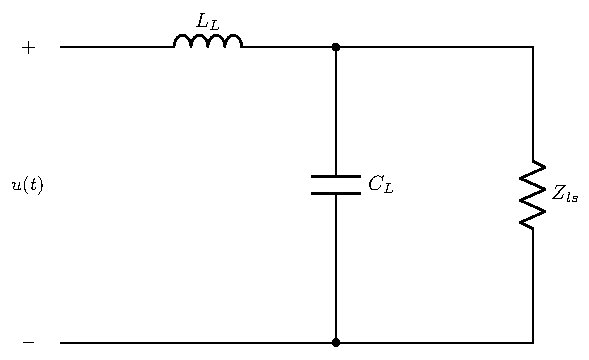
\includegraphics[width=\linewidth]{TU Delft Booming Bass Project Report/figures/FilterGroup/Low pass filter schematic.pdf}
        \captionsetup{justification=centering}
        \subcaption{Low-pass filter schematic.}
        \label{fig:LowPassFilter}
    \end{minipage}%
    \hfill
    \begin{minipage}{0.36\textwidth}
        \centering
        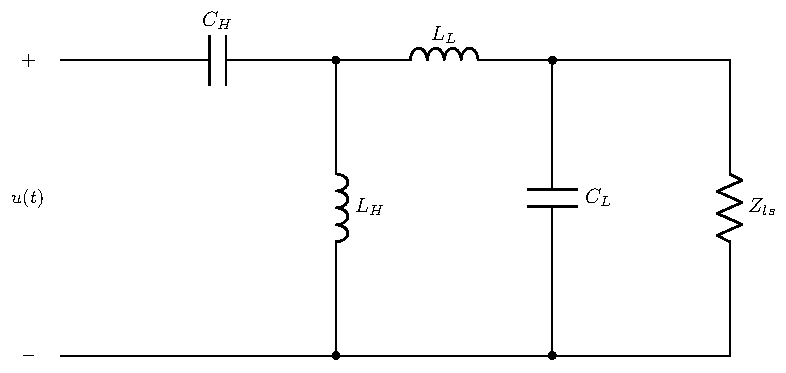
\includegraphics[width=\linewidth]{TU Delft Booming Bass Project Report/figures/FilterGroup/Band pass filter schematic.pdf}
        \captionsetup{justification=centering}
        \subcaption{Band-pass filter schematic.}
        \label{fig:BandPassFilter}
    \end{minipage}
    \captionsetup{justification=raggedright, labelfont=bf}
    \caption{Schematics of different filters used in the project. (a) High-pass filter, with components $C_H$ and $L_H$ representing the HPF capacitance and inductance. (b) A low-pass filter (LPF), where $C_L$ and $L_L$ are the LPF capacitance and inductance. (c) A band-pass filter (BPF), designed by combining the characteristics of both HPF and LPF to achieve the desired frequency separation. These schematics illustrate the design of the three filters implemented to optimize the frequency response for the sound amplifying system.}
    \label{fig:FilterSchematics}
\end{figure}



\subsubsection{Component Value Calculations}
To build the filters, the specific values of the components must be found. The values of the components change the cut-off frequencies of the filters. Eq \ref{Cutoff frequency formula} can be used to find the cut-off frequency for a second-order filter. Therefore the right components must be chosen to have the right cut-off frequencies. 

Python was used to find the values of the components that would give a cut-off frequency as close as possible to the decided frequency. As seen in appendix \ref{chapter: Code}, there was a list of available values that was iterated through. It would calculate the cut-off frequency with Eq \ref{Cutoff frequency formula} and store the difference it had with the desired cut-off frequency. This was compared to the next pair until the best pair of inductor and capacitor for both high pass and low pass filters was found. 
\begin{flalign}
    \label{Cutoff frequency formula}
    f_c = \frac{1}{2\pi\sqrt{LC}}
    \equnit{\si{Hz}}
\end{flalign}

When the component values were found, the filters were tested in LTSpice. It was then found that the components were a successful match, as the cut-off frequencies matched the desired ones closely. This allowed the filters to be built and tested in real. 

\chapter{Simulations}
\label{chapter:simulations}
\section{Introduction to Simulations}
Simulating the various sub-circuits of the amplifier system is crucial to minimize unnecessary trial and error. Utilizing circuit simulation software, such as LTSpice, offers valuable insights into the system's behaviour that go beyond what can be achieved through manual calculations. Simulations enable the creation of different plots, which help validate and reinforce design decisions.

\section{Simulations and Results}


\subsection{Power Supply}
\subsubsection{Simulated Power Supply Analysis}
Analysis of the LTSpice simulations was initialized using the values partially gained from calculations \ref{DischargeResistor} and \ref{CapacitanceEquation}, although real-world availability of these values wasn't possible. Therefore, deviations were made from the values presented previously; for the capacitor, a value of 6800$\mu$F was chosen (limited by the range of available smoothing capacitor values and considerations related to inrush current) since a higher capacitance results in a lower ripple percentage. A value of 3.9k$\Omega$ was chosen for the discharge resistors since a smaller resistance results in a shorter discharge time after the operation and minimizes the risk of excessive power dissipation that could potentially damage the resistor when using even smaller values, and due to other previously mentioned effects with the sizing of discharge resistors, where the discharge resistance could have influenced the ripple voltage, even if this effect would be negligible.
\begin{figure}[H]
    \centering
    \captionsetup{justification=raggedright, labelfont=bf}
    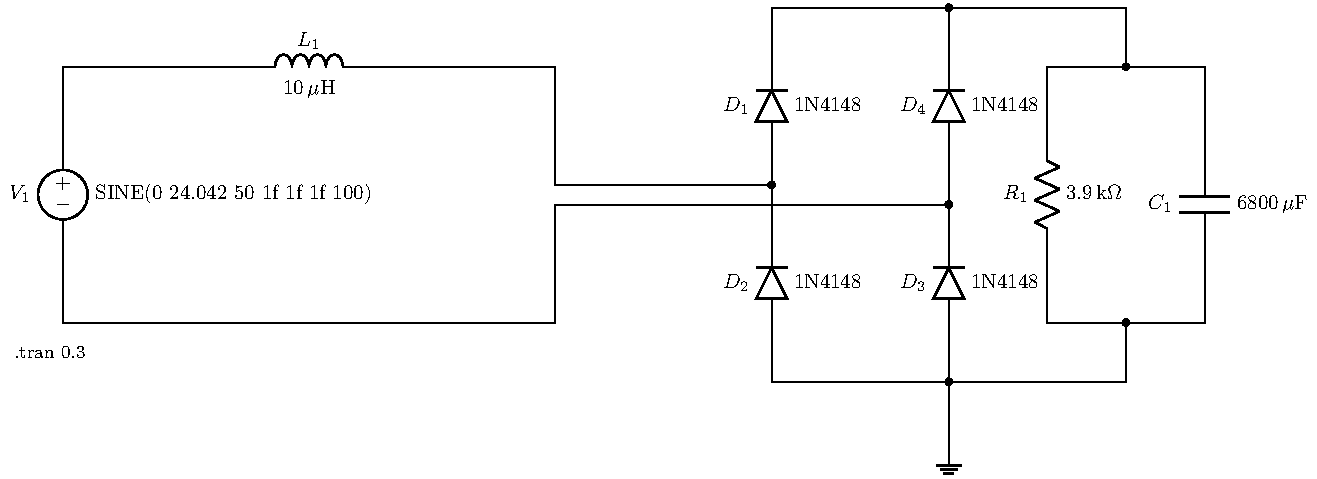
\includegraphics[width=0.8\linewidth]{TU Delft Booming Bass Project Report/figures/PowerSupply/MainPowerSupplyLTSPice.pdf}
    \caption{{LTSpice circuit. For simplicity, only one side of the power supply design is considered, as the transformer is symmetrical on its output terminals. A voltage source is employed at $V_1$ to represent the input voltage (230V,50Hz) with (24.42V, 50Hz) as the specified parameters. This configuration ensures that the resultant voltage and current after the rectification process are consistent with the behavior of a properly modelled transformer.}}
    \label{fig:MainPowerSupplySchematicLTSpice}
\end{figure}

As previously discussed, the LTSpice simulations were performed for only one output terminal, as the use of a center-tapped transformed allows the existence of symmetry of the power supply; this ensures consistent behaviour on both the positive and negative output terminals. This means that analysis on only one side of the output terminal is sufficient. Next to that, the transformer was replaced by an AC voltage source with an inductor in series to model the non-ideal transformer. The model of the circuit used in LTSpice can be seen in \sfautoref{fig:MainPowerSupplySchematicLTSpice}.

\begin{figure}[H]
    \centering
    \captionsetup{justification=raggedright, labelfont=bf}
    \resizebox{0.9\columnwidth}{!}{%
        \begin{tikzpicture} 
            \pgfplotsset{
                every axis legend/.append style={at={(0.98,0.02)}, anchor=south east, legend columns=1},
                every axis/.append style={
                    grid=major,
                    grid style={line width=0.5pt, draw opacity=0.4},
                    tick align=inside, % Ticks will now be inside the plot
                    minor tick num=5
                }
            }
            \begin{axis} [
                xlabel={Time [s]}, % Adjusted x-axis label
                ylabel={$V_{\text{out}}$ [V]},
                title={Effect of different load resistances on $V_{\text{out}}$},
                width=\textwidth,
                height=0.6\textwidth,
                xticklabel style={/pgf/number format/.cd, fixed, precision=3}, % Force fixed-point notation
                scaled x ticks=false, % Disable automatic scaling
                xtick scale label code/.code={}, % Ensure no scale label is shown
                enlargelimits=true % Ensure the graph has enough space for ticks
            ]
                % Plot with 19Ω
                \addplot+[black, no markers] 
                    table [x=time, y=V(n001), col sep=comma] 
                    {TU Delft Booming Bass Project Report/appendix/csv/sim/filtered19ohm_data.txt};
                \addlegendentry{$V_{\text{out}}$ with 19$\Omega$}

                % Plot with 38Ω
                \addplot+[blue, no markers] 
                    table [x=time, y=V(n001), col sep=comma] 
                    {TU Delft Booming Bass Project Report/appendix/csv/sim/filtered38ohm_data.txt};
                \addlegendentry{$V_{\text{out}}$ with 38$\Omega$}

                % Plot with 76Ω
                \addplot+[red, no markers] 
                    table [x=time, y=V(n001), col sep=comma] 
                    {TU Delft Booming Bass Project Report/appendix/csv/sim/filtered76ohm_data.txt};
                \addlegendentry{$V_{\text{out}}$ with 76$\Omega$}

                % Plot with no load
                \addplot+[green, no markers] 
                    table [x=time, y=V(n001), col sep=comma] 
                    {TU Delft Booming Bass Project Report/appendix/csv/sim/filterednoload2_data.txt};
                \addlegendentry{$V_{\text{out}}$ with no load}
            \end{axis}
        \end{tikzpicture}%
    }

    \caption{The simulated circuit output voltage for different load resistances. The black line represents the circuit with 19$\Omega$, the blue line with 38$\Omega$, the red line with 76$\Omega$, and the green line with no load.}
    \label{fig:OutputVoltageWith-Without}
\end{figure}


\begin{figure}[H]
    \centering
    \begin{minipage}{0.48\textwidth}
        \centering
        \captionsetup{justification=raggedright, labelfont=bf}
        \caption{Simulation characteristics of the power supply under varying load levels, displaying the average output voltage, current, and ripple percentage for each load condition. A graphical representation of this data is shown in \sfautoref{fig:OutputVoltageRipplePower}. The results highlight the performance of the power supply across different load resistances, with notable variations in ripple percentage and system stability as the load conditions change.}
        \begin{threeparttable}
          \centering
          \begin{tabular}{c @{\hspace{12pt}} *4{c} S @{\hspace{12pt}}}
            \toprule
            \multicolumn{5}{c}{\textbf{Simulated Power Supply Characteristics}} \\
            \cmidrule(lr){1-5}
            & & \multicolumn{3}{c}{\textbf{Performance Metrics}} \\
            \cmidrule(lr){3-5}
            & $R_\text{Load}$ [$\Omega$] & $V_\text{Av.}$ [V] & $I_\text{res}$ [A] & $u_\text{ripple}$ [\%] \\
            \midrule
            1 & 19 & 18.3 & 0.963 & 2.58 \\
            2 & 38 & 19.6 & 0.516 & 1.43 \\
            3 & 76 & 20.5 & 0.27 & 0.78 \\
            4 & Open & 22.3 & 0.00 & 0.55 \\
            \bottomrule
          \end{tabular}
        \end{threeparttable}
        
        \label{tab:CharacteristicsSim}
    \end{minipage}\hfill
    \begin{minipage}{0.48\textwidth}
        \centering
        \resizebox{\linewidth}{!}{%
            \begin{tikzpicture} 
                \pgfplotsset{
                    every axis legend/.append style={ at={(0.02,0.98)}, anchor=north west, legend columns = 1}, 
                    every axis/.append style={ytick distance=0.5, xtick distance=2, minor tick num=1, grid=major,
                    every axis grid/.append style={line width=0.5pt, draw opacity=0.4}}}
                    \begin{axis} [xlabel = {Delivered power [W]}, ylabel = {Ripple [\%]}]
                        \addlegendentry{Ripple [\%]}
                        \addplot+[no markers] table[row sep=crcr] {
                            {Supplied Power (W):}       {Ripple(\%):} \\
                            17.63       2.58  \\
                            10.11     1.43  \\
                            5.54     0.78  \\
                            0     0.55  \\
                        };
                    \end{axis}
            \end{tikzpicture}%
        }
        \captionsetup{justification=raggedright, labelfont=bf}
        \caption{The output voltage ripple as a function of the power delivered to varying load resistances, illustrating and highlighting the variations in ripple in response to changes in load power.}
        \label{fig:OutputVoltageRipplePower}
    \end{minipage}
\end{figure}

Table \ref{tab:CharacteristicsSim} presents the simulation results for the power supply operating under different resistive load conditions. The presented data includes each load scenario's corresponding average output voltage, current, and ripple percentage. The ripple percentage was determined using \seautoref{RippleVoltageEquation}. All the values were obtained through computational analysis, with the detailed code provided in the appendix. These results offer a comprehensive evaluation of the power supply's performance across different load levels, highlighting its capability to deliver stable output and maintain consistent performance under varying operating conditions.
\begin{figure}[H]
    \centering
    \captionsetup{justification=raggedright, labelfont=bf}
    \resizebox{0.9\columnwidth}{!}{%
        \begin{tikzpicture} 
            \pgfplotsset{
                every axis legend/.append style={at={(0.98,0.02)}, anchor=south east, legend columns=1},
                every axis/.append style={
                    grid=major,
                    grid style={line width=0.5pt, draw opacity=0.4},
                    tick align=inside, % Ticks will now be inside the plot
                    minor tick num=5
                }
            }
            \begin{axis} [
                xlabel={Time [s]}, % Adjusted x-axis label
                ylabel={$V_{\text{out}}$ [V]},
                title={Effect of the smoothing capacitors on $V_{\text{out}}$},
                width=\textwidth,
                height=0.6\textwidth,
                xticklabel style={/pgf/number format/.cd, fixed, fixed zerofill, precision=3}, % Force fixed-point notation
                scaled x ticks=false, % Disable automatic scaling
                xtick scale label code/.code={}, % Ensure no scale label is shown
                enlargelimits=true % Ensure the graph has enough space for ticks
            ]
                % Plot with capacitors
                \addplot+[black, no markers] 
                    table [x={time}, y={V(n001)}, col sep=comma, mark=none] 
                    {TU Delft Booming Bass Project Report/appendix/csv/sim/filtered_data.txt};
                \addlegendentry{$V_{\text{out}}$ with capacitors}
                
                % Plot without capacitors
                \addplot+[blue, no markers] 
                    table [x={time}, y={V(n005)}, col sep=comma, mark=none] 
                    {TU Delft Booming Bass Project Report/appendix/csv/sim/filtered_data.txt};
                \addlegendentry{$V_{\text{out}}$ without capacitors}
            \end{axis}
        \end{tikzpicture}%
    }

    \caption{{The simulated circuit output voltage. The blue line represents the circuit without smoothing capacitors, while the black line shows the circuit with the 6.8$\mu$F smoothing capacitors in place.}}
    \label{fig:OutputVoltageWith-Without}
\end{figure}

Without a smoothing capacitor, the full-wave rectified waveform exhibits a ripple, with oscillations in voltage that follow the rectified signal. The absence of smoothing capacitors results in "negative" voltage dips between the peaks, as the diode stops conducting the during rectification process, creating a brief dip to zero or even negative. These negative voltages, as seen in Fig. \ref{fig:OutputVoltageWith-Without}, could also arise from minor errors or deviations in the measurement setup. Additionally, the behavior of the diodes may contribute to these negative readings. When the input voltage is near zero, the forward voltage drop of the diodes can cause the output to become negative until the input voltage exceeds the threshold required for conduction. This results in small negative spikes, particularly under low load or near-zero input conditions.
\begin{figure}[H]
    \centering
    \captionsetup{justification=raggedright, labelfont=bf}
    \resizebox{0.9\columnwidth}{!}{%
        \begin{tikzpicture} 
            \pgfplotsset{
                every axis legend/.append style={at={(0.98,0.02)}, anchor=south east, legend columns=1},
                every axis/.append style={
                    grid=major,
                    grid style={line width=0.5pt, draw opacity=0.4},
                    tick align=inside, % Ticks will now be inside the plot
                    minor tick num=5
                    }
            }
            \begin{axis} [
                title={Effect of the smoothing capacitors on $I_T$},
                xlabel={Time [s]},
                ylabel={$I_T$ [A]},
                width=\textwidth,
                height=0.6\textwidth,
                xticklabel style={/pgf/number format/.cd, fixed, fixed zerofill, precision=3}, % Force fixed-point notation
                scaled x ticks=false, % Disable automatic scaling
                xtick scale label code/.code={}, % Ensure no scale label is shown
                enlargelimits=true % Ensure the graph has enough space for ticks
            ]
                % Plot with capacitors
                \addplot+[black, no markers] 
                    table [x={time}, y={I(L1)}, col sep=comma, mark=none] 
                    {TU Delft Booming Bass Project Report/appendix/csv/sim/filteredcurrent_data.txt};
                \addlegendentry{$I_T$ with capacitors}
                
                % Plot without capacitors
                \addplot+[blue, no markers] 
                    table [x={time}, y={I(L2)}, col sep=comma, mark=none] 
                    {TU Delft Booming Bass Project Report/appendix/csv/sim/filteredcurrent_data.txt};
                \addlegendentry{$I_T$ without capacitors}
            \end{axis}
        \end{tikzpicture}%
    }
    \caption{{The simulated circuit current through the transformer. The blue line represents the circuit without smoothing capacitors, while the black line represents the circuit with the capacitors. As observed and mentioned before, the inclusion of the smoothing capacitor $C_1$ leads to an increase in the initial current, commonly referred to as the rush-in current. }}
    \label{fig:OutputCurrenteWith-Without}
\end{figure}

Fig. \ref{fig:OutputVoltageWith-Without} and \ref{fig:OutputCurrenteWith-Without} clearly demonstrate the impact of the smoothing capacitors on the output voltage and current waveforms. In figure \ref{fig:OutputVoltageWith-Without}, the absence of smoothing capacitors results in the output voltage remaining a rectified sinusoidal shape. Conversely, the inclusion of smoothing capacitors produces an output voltage waveform that resembles a steady DC voltage signal a lot closer. 

\subsection{Power Amplifier}
\label{section: sim PA}
The circuit diagram of the ideal power amplifier circuit is shown in \sfautoref{fig:ideal amplifier}, where $\mathbf{V_{out}}$ is the output of the power amplifier and $\mathbf{V_{in}}$ the signal received from the computer:
\begin{figure}[H]
    \centering
    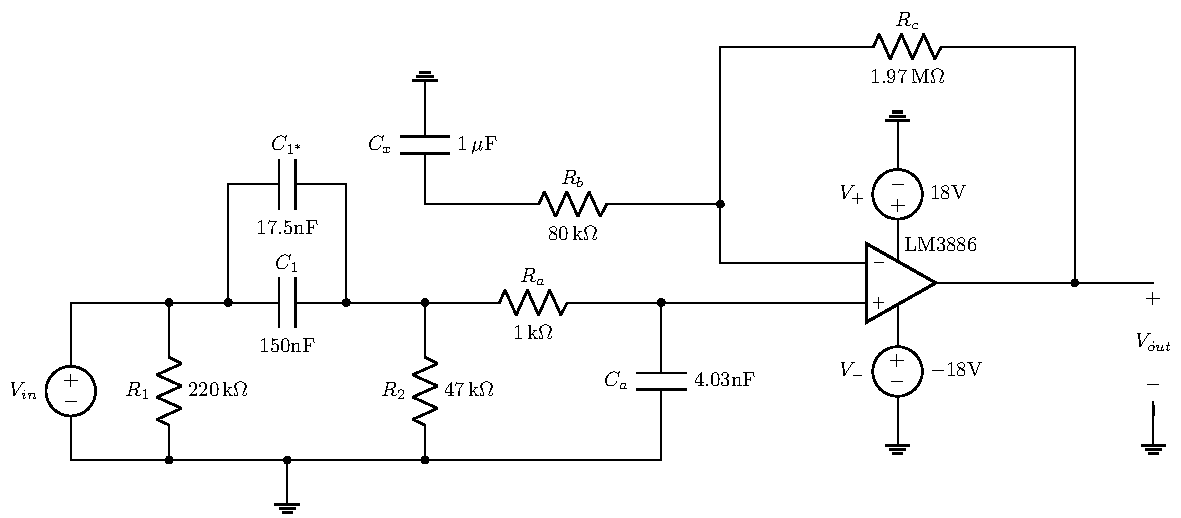
\includegraphics[width=0.9\linewidth]{TU Delft Booming Bass Project Report/figures/PowerAmplifier/circuits/ideal amplifier.pdf}
    \captionsetup{justification=raggedright, labelfont=bf}
    \caption{The ideal power amplifier circuit, where "ideal" refers to the component values leading to a simulation where the frequency response exactly matches the requirements given in \autoref{requirements PA}}
    \label{fig:ideal amplifier}
\end{figure}

To obtain a comprehensive understanding of the circuit's behavior, a frequency sweep from 1Hz to 1MHz was conducted. Simulations of the circuit, using the ideal parameters and values listed in \stautoref{tab:B2-1 ideal values}, indicated that the design requirements were not met (see \sfautoref{fig:not ideal amplifier}). After adjusting the component values to the ideal values in \stautoref{tab: B2-1 actual ideal values}, the bode plot in \sfautoref{fig: ideal amp results} was obtained. The ideal power amplifier simulation utilizes the component values to obtain an ideal frequency response, while the real amplifier operates with the used values from \stautoref{tab: B2-1 actual ideal values}. The frequency response of the real power amplifier is shown in \sfautoref{fig:real circuit results}
\begin{figure}[H]
  \centering
    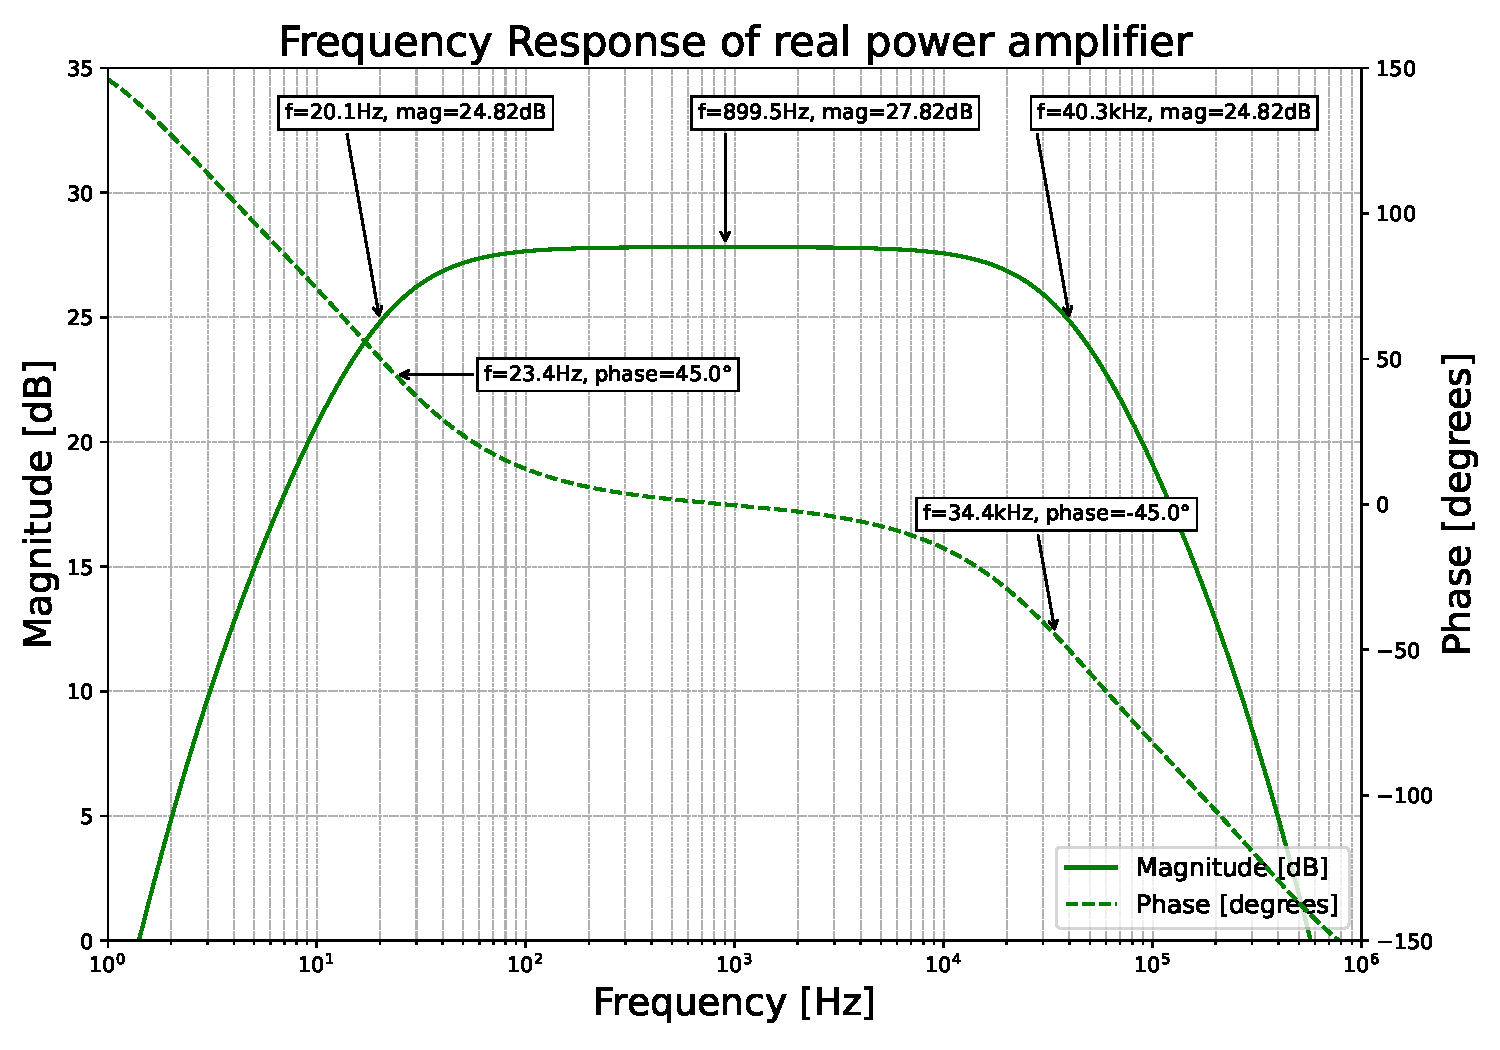
\includegraphics[width=0.75\linewidth]{TU Delft Booming Bass Project Report/figures/PowerAmplifier/real power amplifier results.pdf}
    \captionsetup{justification=raggedright, labelfont=bf}
    \caption{The frequency response of the real power amplifier circuit. As can be seen, the real power amplifier features corner frequencies at around 20.1Hz and 40.3kHz, while maintaining a maximum gain of 27.82dB at a frequency of 899.5Hz.}
    \label{fig:real circuit results}
\end{figure}
\begin{figure}[H]
    \centering
    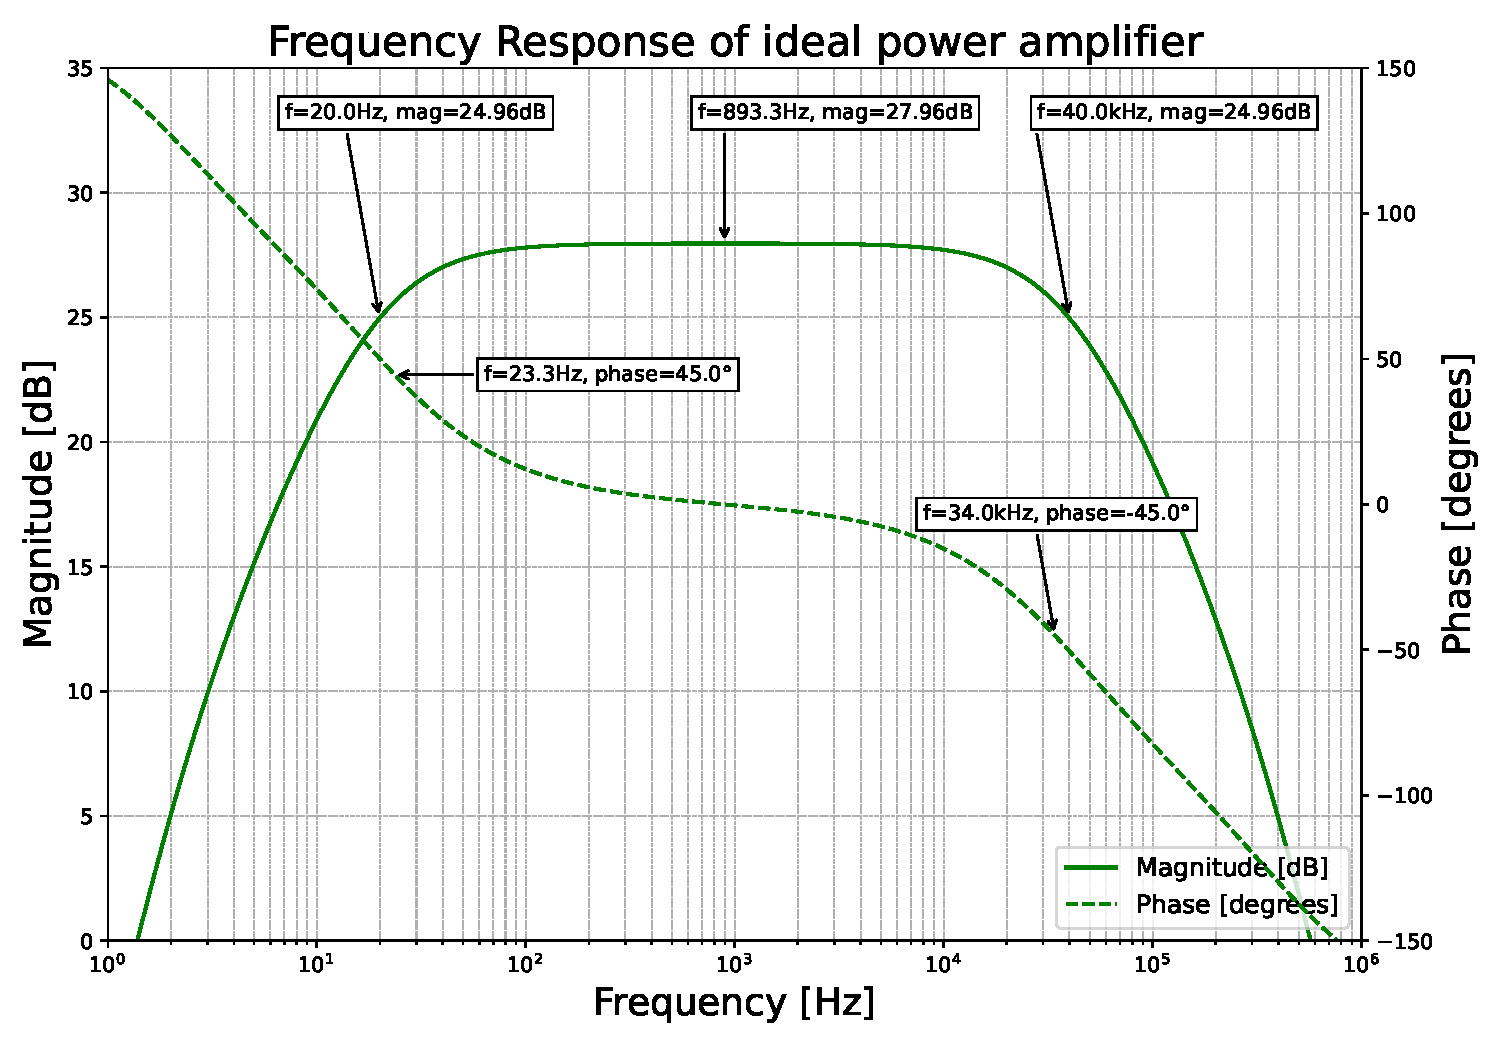
\includegraphics[width=0.75\linewidth]{TU Delft Booming Bass Project Report/figures/PowerAmplifier/ideal power amplifier results.pdf}
    \caption{The ideal frequency response of the power amplifier circuit. As observed, the ideal power amplifier exhibits corner frequencies at 20Hz and 40.0kHz, while maintaining a maximum gain of 27.96dB.}
    \label{fig: ideal amp results}
\end{figure}



\sfautoref{fig: ideal amp results} illustrates that the ideal power amplifier circuit features corner frequencies of 20Hz and 40kHz, with a gain of 27.96dB. In comparison, the real amplifier circuit exhibits corner frequencies of 20.1Hz and 40.3kHz, along with a gain of 27.82dB. In \stautoref{tab: B2-1 actual ideal values}, all of the eventual component values can be seen, along with the deviation between the used values in the real amplifier circuit and both the calculated ideal values and simulated ideal values, respectively.

\begin{table}[H]
    \centering
    \captionsetup{justification=raggedright, labelfont=bf}
    \caption{B2-1 Summary of the calculated ideal values and the corresponding actual-ideal values (Resistance $R_N$, capacitance $C_N$, cut-off frequency $f_{\text{cut-off}}$, and the gain $\mathbf{G_{\text{dB}}}$) based on simulation results. The table includes values for the p-HPF, p-LPF, and a-HPF, with $D_{\text{diff} 1}[\%]$ representing the deviation between the calculated ideal and used values, and $D_{\text{diff} 2}[\%]$ representing the deviation between the simulated ideal and used values.}
    \resizebox{\textwidth}{!}{
    \begin{tabular}{c @{\hspace{12pt}} *7{c} S @{\hspace{12pt}}}
        \toprule
        \multicolumn{7}{c}{\textbf{B2-1 Filter Component Parameters}} \\
        \cmidrule(lr){1-7}
       
        & Parameter & Calculated Value & Ideal Value & Used Value & D$_{\text{diff} 1}$ [\%] & D$_{\text{diff} 2}$ [\%]  \\
        \midrule
        p-HPF & $R_2$ [$\Omega$] & 47k$\Omega$ & 47k$\Omega$ &  47k$\Omega$ &0.00\%  & 0.00\% \\
         & $C_1$ [F] & 169.3nF & 167.5nF &166.5nF & -1.68\%&  -0.60\% \vspace{4pt} \\
         & $f_\text{cut-off}$ [Hz] & 19.8Hz & 20Hz &20.1Hz & 1.50\% &  0.50\% \vspace{10pt} \\
        p-LPF & $R_a$ [$\Omega$] & 1k$\Omega$ &  1k$\Omega$ & 987$\Omega$ & -1.30\%  & -1.30\% \\
         & $C_a$ [F] & 3.98nF & 4.03nF & 4.05nF & 1.76\%& 0.50\%    \vspace{4pt}\\
         & $f_\text{cut-off}$ [Hz] & 40.5kHz & 40kHz & 40.3kHz & -0.50\% & 0.75\% \vspace{10pt}\\
        a-HPF &  $R_b$[$\Omega$] & 80k$\Omega$ & 80k$\Omega$ & 81.8k$\Omega$ & 2.25\% & 2.25\%  \\
        & $R_c$ [$\Omega$] & 1.92M$\Omega$ & 1.97M$\Omega$ & 1.98M$\Omega$ & 3.13\% &  0.51\% \\
         & $C_x$ [F] & 1$\mu$F & 1$\mu$F & 968nF & -3.31\%  &  -3.31\%  \vspace{4pt} \\
         & $\mathbf{G_{\text{dB}}}$  & 27.76dB & 27.96dB & 27.82dB & 0.22\% &  -0.50\%  \\
        \bottomrule
    \end{tabular}
    }
    
    \label{tab: B2-1 actual ideal values}
\end{table}

\subsubsection{Results of B2-2}
As illustrated in \sfautoref{fig: Alternative frequency response output}, using the Used values shown in \autoref{tab:B2-1 ideal values}, the corner frequencies achieved in the simulations for B2-2's design were 20Hz and 36kHz:

\begin{figure}[H]
    \centering
    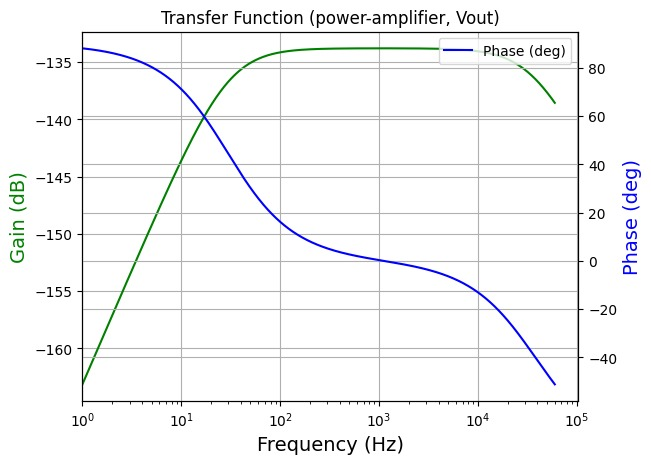
\includegraphics[width=0.75\linewidth]{TU Delft Booming Bass Project Report/figures/PowerAmplifier/Vout alternative design.jpg}
    \captionsetup{justification=raggedright, labelfont=bf}
    \caption{The frequency response of B2-2's power amplifier circuit, with corner frequencies at around 20Hz and 36kHz.}
    \label{fig: Alternative frequency response output}
\end{figure}

\subsection{Filters}
\subsubsection{Simulation of the passive filters}
In order to verify that the calculated component values of the filters produce transfer functions that closely match the desired transfer functions, the designed circuits (\sfautoref{fig:FilterSchematics}) were first individually simulated inside the circuit simulation tool LTSpice. After the individual transfer functions were confirmed to produce the expected results by demonstrating the behavior characteristic of each respective filter. The circuits of all three filters (\sfautoref{fig:FilterSchematics}) with \(R_{ls}\) as the respective speaker's impedance model and with components values from \stautoref{tab:filter_components} were simulated together and tuned further to each other to produce the summed frequency response graph as seen in
\sfautoref{fig:freq_resp}:
\begin{figure}[H]
    \centering
        \begin{minipage}{0.48\textwidth}
            \begin{figure}[H]
            \centering
            \captionsetup{justification=raggedright, labelfont=}
                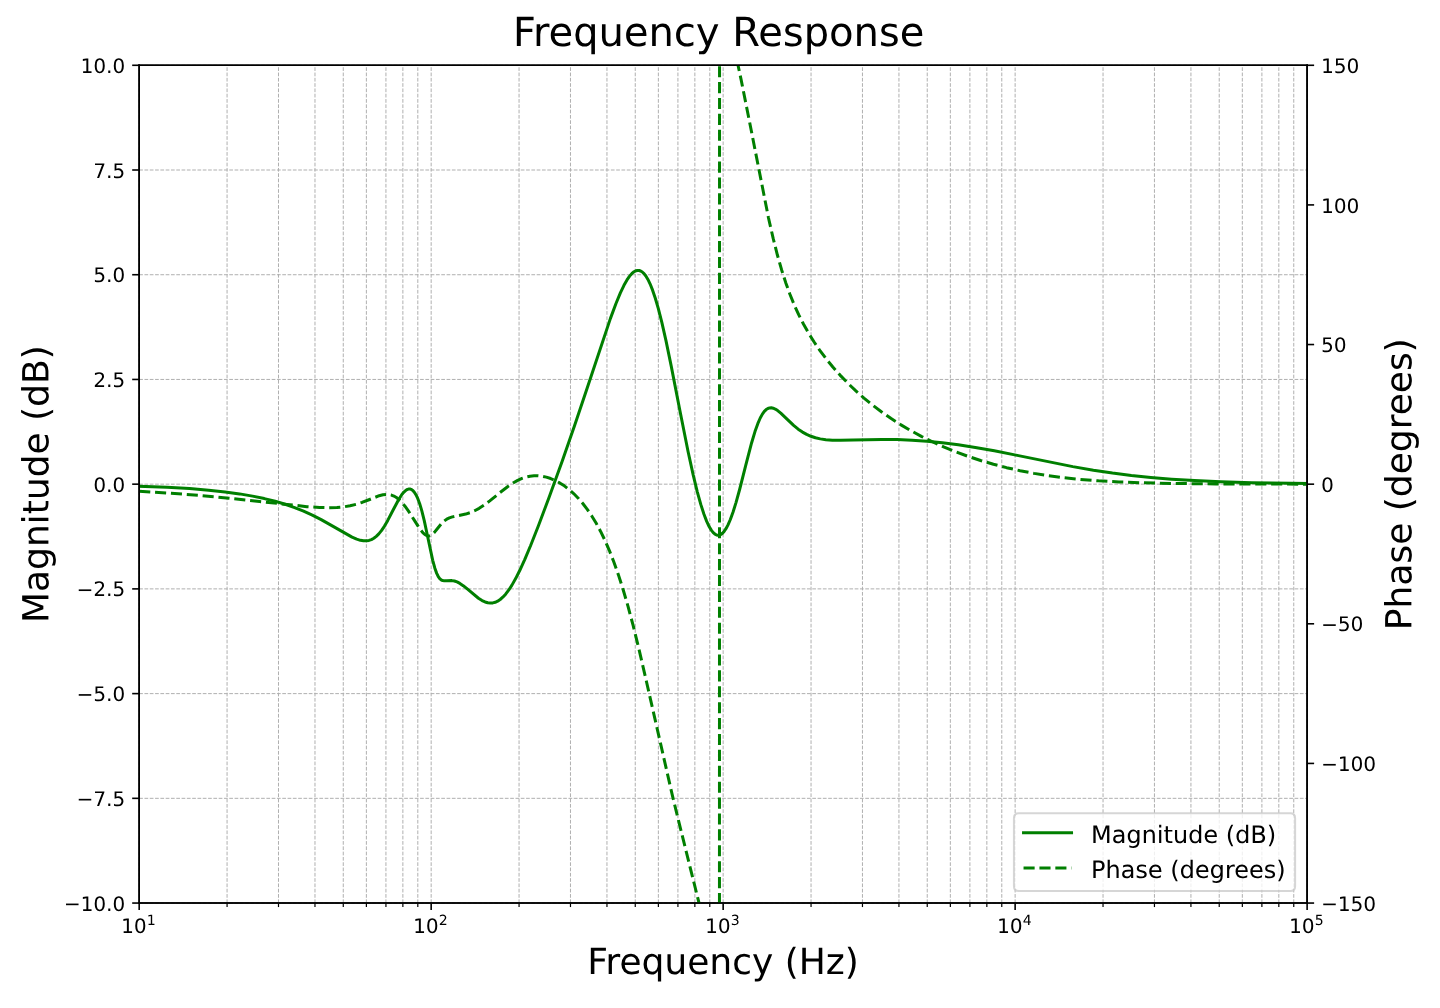
\includegraphics[width=0.9\linewidth]{TU Delft Booming Bass Project Report//figures//FilterGroup/Frequency response.png}
            \caption{Frequency response of the filter bank.}
            \label{fig:freq_resp}
            \end{figure}
        \end{minipage}
        \hfill % Add space between the two mini pages
        \begin{minipage}{0.50\textwidth}
        \captionsetup{justification=raggedright, labelfont=bf}
        \captionof{table}{Values of components for each filter type.}
            \centering
            \begin{tabular}{@{}lccc@{}}
            \toprule
    \textbf{Filter Type}     & \textbf{Component} & \textbf{Value} \\ \midrule
    \multirow{2}{*}{HPF} 
                             & Capacitor                & 28.8 $\mu$F      \\
                             & Inductor                & 0.47 mH        \\ \midrule
    \multirow{2}{*}{Low-Pass of BPF}
                            & Inductor              & 0.67 mH \\
                            & Capacitor             & 100 $\mu$F \\
                            \midrule
    \multirow{2}{*}{High-Pass of BPF}
                            & Capacitor              & 147 $\mu$F \\
                            & Inductor             & 4.7 mH \\
                            \midrule
    
    \multirow{2}{*}{LPF} 
                             & Inductor                & 2.88 mH         \\
                             & Capacitor                 & 100 $\mu$F     \\ \bottomrule
    \end{tabular}
    
        \label{tab:filter_components}
    \end{minipage}
\end{figure}


As seen in \sfautoref{fig:freq_resp}, the frequency response is not     completely flat and has a maximum deviation of 5.0dB at 510Hz; this was found to be acceptable as further altering the values of the components only had a negative effect by shifting the cut-off frequencies to an undesirable range.



\subsection{Loudspeakers}
Using the formulas derived from the circuit model, the corresponding component values can be found for each speaker. The calculations were done for each speaker by their respective filter group, which resulted in the component values found in \stautoref{tab:speaker_components}. 

Using the parameters found, the frequency response of each model was calculated and compared with the measured speaker data. This showed that the model matched closely around the resonance peak but generally had a slightly lower impedance than the measured data, as seen in Fig. \ref{fig:/model vs measured impedance}. 

\begin{figure}[H]
    \centering
    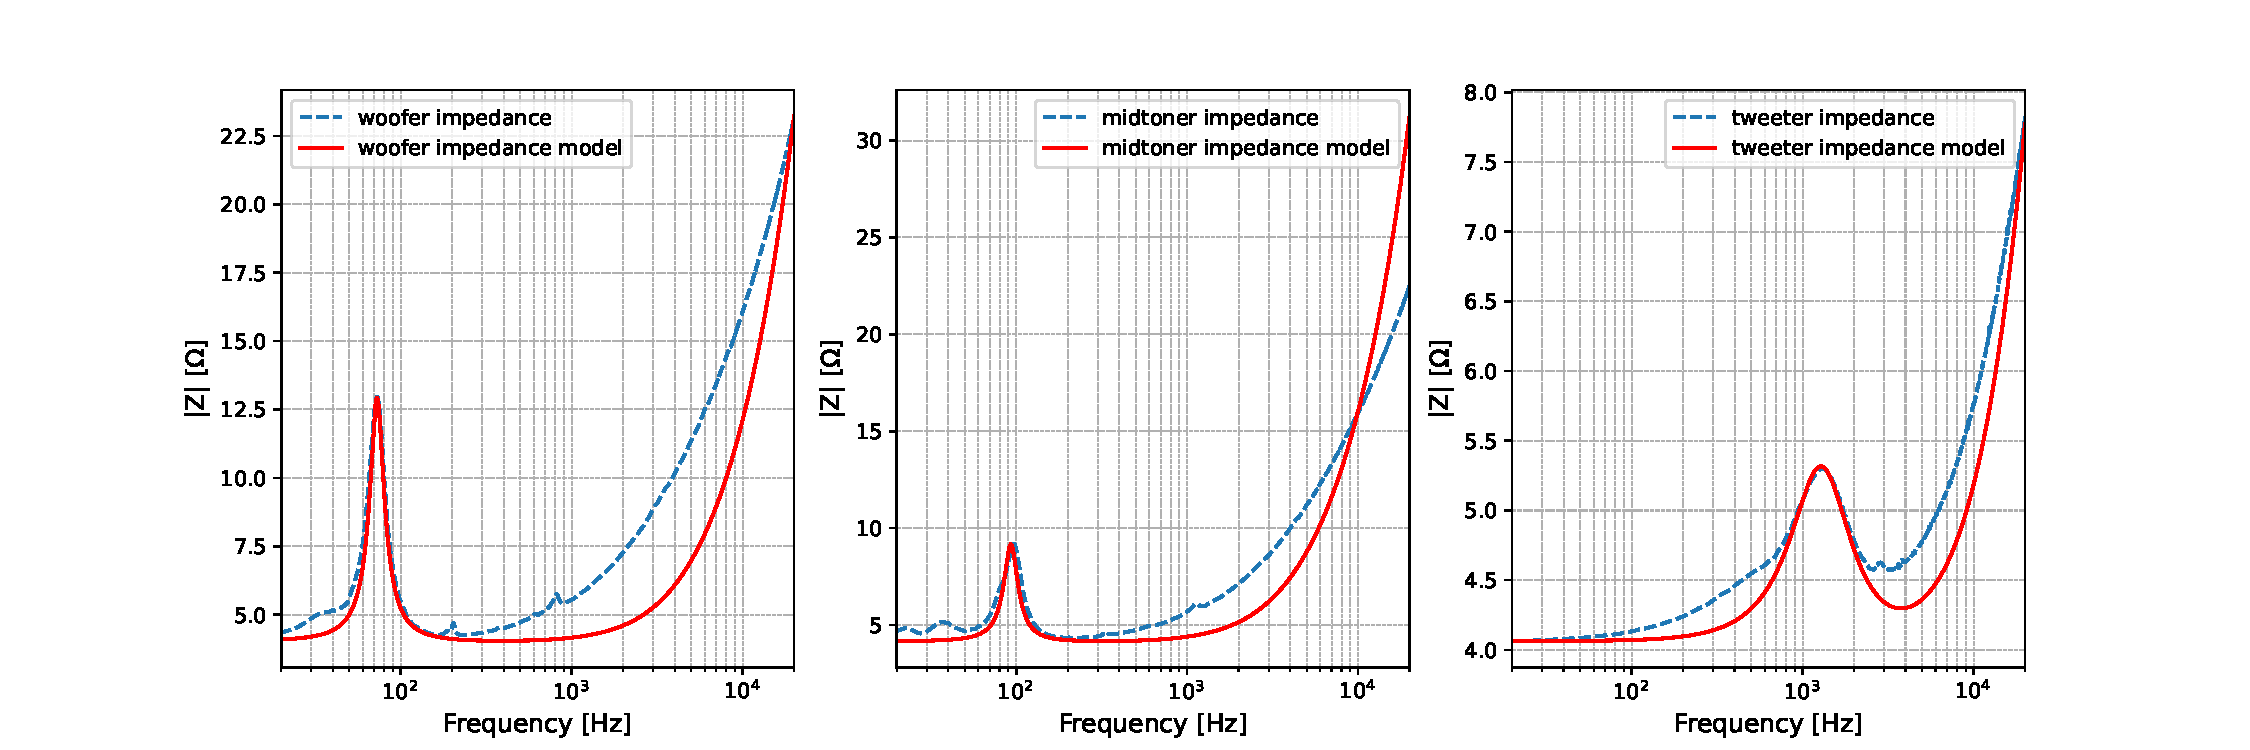
\includegraphics[width=1\textwidth]{TU Delft Booming Bass Project Report/figures/FilterGroup/model vs measured impedance.pdf}
    \captionsetup{justification=raggedright, labelfont=bf}
    \caption{Model speaker impedance versus measured speaker impedance}
    \label{fig:/model vs measured impedance}
\end{figure}

\section{Discussion}

\subsection{Power supply}
The simulations of our circuit are designed to be as accurate as possible. However, since LTSpice may not fully replicate real-world conditions, unexpected differences can arise in practical applications. These discrepancies will be analyzed further in Chapter \ref{subsec:psdiscussion}.


\subsection{Power amplifier}
The circuit with the calculated ideal values probably gives a different result in the simulation than would be expected because LTSpice does take into account the interference between filters, which eventually impacts the frequency response. While in the calculations, all filters were taken separately, as if the interference did not occur. 

The simulations clearly demonstrate that the deviation between the values used in the final circuit is generally closer to the ideal simulated values than to the calculated ideal values. This suggests that the end product is likely to perform in closer alignment with the ideal simulation.

For B2-2's design, it is unclear what the exact amplification is; this may be fixed by using another power amplifier in the simulation. That could be the cause for ending at -135dB. B2-1 used a universal opamp, which did not have this issue.
\subsection{Filters}
During the simulation of the filters, idealized component values were used (e.g. Inductors and Capacitors with no real resistance) as this would greatly simplify the analysis and design process. This clearly differs from real-world circumstances, which would change the transfer function and, thus, the real-life frequency response. 

\subsection{Loudspeakers}
The loudspeaker model is a very simplified version of real-world circumstances. With the entire speaker system being modeled by 5 components, its frequency response will clearly differ from those of the measured speaker data. 

For a more accurate description, a more complex model could have been used, but this, in turn, would have required us to differ from the one in the manual and find or create a new model, and it would have made calculating the model parameters a more arduous task. 
\chapter{Measurements}
\label{chapter:measurements}
\section{Introduction to Measurements}
Measuring a design gives real-world insight into the success of a design of a component. Circuit theory does not always match what happens in the real world, as assumptions are made to simplify models on paper. Therefore, testing and measuring real-world data is essential to the design of a system, as it can point out flaws in the assumptions made by the theory. This, therefore, allows for adjustments to be made, which would only be found by measuring.

\section{Measurements Results}
\subsection{Power Supply}
The voltage waveform across load resistors $R_{\text{load},1}$ and $R_{\text{load},2}$ were measured under four distinct conditions to evaluate the ripple voltage. During these measurements, only the positive side of the power supply was loaded, as the negative side is an exact replica of the positive side due to the symmetry of a center-tapped transformer (CT-T). The measurements were performed by connecting the probe to both the ground and the positive output of the power supply, denoted by $V_{out}$, with the voltage being measured across the load resistors. These measurements yielded the characteristics shown in Tab. \ref{tab:CharacteristicsSim}. The ripple was calculated using Eq. \ref{RippleVoltageEquation}. The code provided in Appendix \ref{sec:ripvoltcodemea} was utilized to calculate the values presented in Tab. \ref{tab:CharacteristicsSim}.

\begin{figure}[H]
    \centering
    \captionsetup{justification=raggedright, labelfont=bf}
    \resizebox{0.75\columnwidth}{!}{%
        \begin{tikzpicture} 
        \pgfplotsset{
                every axis legend/.append style={at={(0.98,0.02)}, anchor=south east, legend columns=1},
                every axis/.append style={
                    grid=major,
                    grid style={line width=0.5pt, draw opacity=0.4},
                    tick align=inside, % Ticks will now be inside the plot
                    minor tick num=5
                }
            }
            \begin{axis} [
                xlabel={Time [s]}, % Adjusted x-axis label
                ylabel={$V_{\text{out}}$ [V]},
                title={Effect of different load resistances on $V_{\text{out}}$},
                width=\textwidth,
                height=0.6\textwidth,
                xticklabel style={/pgf/number format/.cd, fixed, fixed zerofill, precision=3}, % Force fixed-point notation
                scaled x ticks=false, % Disable automatic scaling
                xtick scale label code/.code={}, % Ensure no scale label is shown
                enlargelimits=true % Ensure the graph has enough space for ticks
            ]
                % Plot for 19Ω
                \addplot+[black, no markers] 
                    table [x=d, y=e, col sep=comma] {TU Delft Booming Bass Project Report/appendix/csv/19 ohm/F0009CH1.CSV};
                \addlegendentry{$V_{\text{out}}$ with 19$\Omega$}

                % Plot for 38Ω
                \addplot+[blue, no markers] 
                    table [x=d, y=e, col sep=comma] {TU Delft Booming Bass Project Report/appendix/csv/38 ohm/F0007CH1.CSV};
                \addlegendentry{$V_{\text{out}}$ with 38$\Omega$}

                % Plot for 76Ω
                \addplot+[red, no markers] 
                    table [x=d, y=e, col sep=comma] {TU Delft Booming Bass Project Report/appendix/csv/76 ohm/F0011CH1.CSV};
                \addlegendentry{$V_{\text{out}}$ with 76$\Omega$}

                % Plot for no load
                \addplot+[green, no markers] 
                    table [x=d, y=e, col sep=comma] {TU Delft Booming Bass Project Report/appendix/csv/No load/F0008CH1.CSV};
                \addlegendentry{$V_{\text{out}}$ with no load}
            \end{axis}
        \end{tikzpicture}%
    }
    \caption{The output voltage $V_{out}$ waveform for various load resistances: 19$\Omega$, 38$\Omega$, 76$\Omega$ and no load. As the load resistance $R_{load}$ increases, the ripple $u_{\text{ripple}}$ decreases. This occurs because a high load resistance reduces the current drawn from the power supply, causing the voltage across the smoothing capacitor to remain more stable and preventing large fluctuations in the output voltage. This results in a smaller ripple as the capacitor has more time to charge and discharge gradually.}
    \label{fig:MeasuredLoadOutputVoltage}
\end{figure}


\begin{figure}[H]
    \centering
    \begin{minipage}{0.48\textwidth}
        \centering
        \begin{threeparttable}
          \centering
          \begin{tabular}{c @{\hspace{12pt}} *4{c} S @{\hspace{12pt}}}
            \toprule
            \multicolumn{5}{c}{\textbf{Measured Power Supply Characteristics}} \\
            \cmidrule(lr){1-5}
            & & \multicolumn{3}{c}{\textbf{Performance Metrics}} \\
            \cmidrule(lr){3-5}
            & $R_\text{Load}$ [$\Omega$] & $V_\text{Av.}$ [V] & $I_\text{res}$ [A] & $u_\text{ripple}$ [\%] \\
            \midrule
            1 & 19 & 20.1 & 1.06 & 3.23 \\
            2 & 38 & 21.1 & 0.56 & 1.66 \\
            3 & 76 & 21.9 & 0.29 & 1.10 \\
            4 & Open & 23.0 & 0.00 & 0.26 \\
            \bottomrule
          \end{tabular}
        \end{threeparttable}
        \captionsetup{justification=raggedright, labelfont=bf}
        \caption{Characteristics of the power supply in real-world applications under various load levels, using load resistors equipped with large heatsinks to dissipate the thermal energy from imperfect energy conversion. The data includes each load's average output voltage, current, and ripple percentage.}
        \label{tab:CharacteristicsSim}
    \end{minipage}\hfill
    \begin{minipage}{0.48\textwidth}
        \centering
        \resizebox{\linewidth}{!}{%
            \begin{tikzpicture} 
                \pgfplotsset{
                    every axis legend/.append style={ at={(0.02,0.98)}, anchor=north west, legend columns = 1}, 
                    every axis/.append style={ytick distance=0.25, xtick distance=2, minor tick num=1, grid=major,
                    every axis grid/.append style={line width=0.5pt, draw opacity=0.4}}}
                    \begin{axis} [xlabel = {Delivered power [W]}, ylabel = {Ripple [\%]}]
                        \addlegendentry{Ripple[\%]}
                        \addplot+[no markers] table[row sep=crcr] {
                            Supplied power(W):       Ripple(\%): \\  
                            21.31       3.23  \\
                            11.82     1.66  \\
                            6.351     1.10  \\
                            0     0.26  \\
                        };
                    \end{axis}
            \end{tikzpicture}%
        }
        \captionsetup{justification=raggedright, labelfont=bf}
        \caption{The output voltage ripple as a function of the power delivered to varying load resistances, showing the voltage ripple magnitude and the corresponding load power.}
        \label{fig:OutputVoltageRipplePower}
    \end{minipage}
\end{figure}
The ripple observed for the open circuit is likely due to a measurement error from the oscilloscope, which was set with a resolution of 0.04V. In the measurements, the maximum voltage recorded was 23.04V, while the average voltage was 23.00V. Although a small ripple could have resulted from the capacitors slowly discharging through the discharge resistors, the ripple induced by this current was negligible and thus insignificant compared to the one measured, as the discharge current is very small.
\subsubsection{Discharge Capacitors}

\begin{figure}[H]
    \centering
    \captionsetup{justification=raggedright, labelfont=bf}
    \resizebox{0.9\columnwidth}{!}{%
        \begin{tikzpicture} 
        \pgfplotsset{
                every axis legend/.append style={at={(0.98,0.02)}, anchor=south east, legend columns=1},
                every axis/.append style={
                    grid=major,
                    grid style={line width=0.5pt, draw opacity=0.4},
                    tick align=inside, % Ticks will now be inside the plot
                    minor tick num=5
                }
            }
            \begin{axis} [
                xlabel={Time [s]}, % Adjusted x-axis label
                ylabel={$V_{\text{out}}$ [V]},
                title={Effect of the smoothing capacitors on $V_{\text{out}}$},
                width=\textwidth,
                height=0.6\textwidth,
                xticklabel style={/pgf/number format/.cd, fixed, precision=0}, % Remove decimals by setting precision to 0
                enlargelimits=true % Ensure the graph has enough space for ticks
            ]
                \addplot+[no markers] table [x=d, y=e, col sep=comma] {TU Delft Booming Bass Project Report/appendix/csv/discharge/F0010CH1.CSV};
                \addlegendentry{\(V_{out}\)}
                \addplot[color=red] table[row sep = crcr]{0 8.829 \\ 249.8 8.829 \\};
                \addlegendentry{\(V_{e^{-1}}\)}
            \end{axis}
        \end{tikzpicture}%
    }
    \caption{The discharge curve of the capacitors, measured at $V_{\text{out}}$. The input voltage $V_{in}$ is disconnected from the power supply circuit at $t=33.0\text{s}$}
    \label{fig:dischargeCurve}
\end{figure}

From \autoref{fig:dischargeCurve}, it is evident that the capacitors are disconnected from the power supply at approximately $t=33.0\text{s}$. The discharge curve intersects the red line - indicating the point where $\tau=1$ - at around $\tau\approx 62\text{s}$. This implies that the time constant $\tau$ is approximately 28 seconds. Based on this, the capacitors are expected to fully discharge after 145 seconds, aligning well with the 2.5-minute discharge limit specified in the design requirements.

\subsection{Power Amplifier}
\label{section: measurements poweramp}
After simulating the circuit in LTSpice, it is crucial to test the power amplifier in a real-world environment to assess its actual performance. To achieve this, measurements must be conducted on the constructed power amplifier circuit. The expected outcome from this measurement is a Bode plot that accurately represents a band-pass filter with a dB gain of 27.82 dB and corner frequencies at 20.1Hz and 40.3kHz, corresponding to the -3dB of the gain. Additionally, it is anticipated that the DC offset of the operational amplifier will be amplified by no more than a factor of 1 in accordance with the design specifications. These measurements will provide valuable insights into the circuit's practical performance, ensuring that the theoretical predictions align with real-world behavior.

During the construction of the circuit, each resistor and capacitor was tested to ensure that the physical components matched the expected values from the simulations and calculations. This step was necessary because the capacitance of a capacitor can vary by approximately 20\% from the labeled value and the value of a resistor can vary anywhere from 0.1\% to 20\%. The measured values for all components can be seen in \stautoref{tab:Real values}. These are the same values as shown in \stautoref{tab: B2-1 actual ideal values} and \stautoref{tab:B2-1 ideal values}.
\begin{table}[H]
    \centering
    \begin{tabular*}{0.35\textwidth}{@{\extracolsep{\fill}} c c @{}}
        \toprule
        \textbf{Component} & \textbf{Value of Component} \\
        \midrule
        \textbf{$C_1$} & 166.5nF \\
        \textbf{$C_a$} & 40.5nF \\ 
        \textbf{$C_x$} & 986nF \\
        \textbf{$R_a$} & 987$\Omega$ \\
        \textbf{$R_b$} & 81.8k$\Omega$ \\
        \textbf{$R_c$} & 1.98M$\Omega$ \\
        \bottomrule
    \end{tabular*}
    \captionsetup{justification=raggedright, labelfont=bf}
    \caption{Values of components used in the constructed power amplifier circuit.}
    \label{tab:Real values}
\end{table}




\subsubsection{Measurement Setup and Procedure}

To perform accurate testing of the power amplifier circuit, conducting measurements in a real-world environment is essential, as simulations alone may not provide a complete representation of the circuit's actual performance. The necessary measurements were taken using the following instruments and components (see \sfautoref{fig:PA test setup} for a schematic of the setup):

\begin{itemize}
    \item \textbf{Oscilloscope: Tektronix TDS 2022B} An oscilloscope is necessary to conduct analysis and measurements after building the power amplifier  to measure parameters such as voltage gain and cutoff frequencies.
    \item \textbf{Function Generator: Tektronix AFG 3021B/C} A function generator is essential for conducting analysis and measurements, as it supplies the necessary input signal to the power amplifier, simulating various operating conditions and frequencies.
    \item \textbf{Power Supply (+15V, -15V)} A dual power supply provides the required positive and negative voltages necessary for the operation of the amplifier.
\end{itemize}

For an accurate Bode plot, measurements were taken from 3Hz to 900kHz. The lower bound of 3Hz was selected as no measurable response was observed at 1Hz and 2Hz. The upper bound of 900kHz was chosen, because at that point the dB gain was negative and any high frequencies would not change the obtained bode plot. The frequency steps were progressively increased with each new power of ten, except in the range between 100Hz and 200Hz, where steps of 10Hz were used. Additionally, an input voltage of 400mV peak-to-peak was set on the function generator, as this represents the maximum allowed voltage for the power amplifier (according to \cite{IP-manual}). However, since the output from the function generator may not match the displayed value exactly, both the function generator and power amplifier outputs were connected to the oscilloscope (as shown in \sfautoref{fig:PA test setup}). A DC offset of 500mV was also applied at the output of the function generator to facilitate testing whether this offset gets amplified.

\begin{figure}[H]
    \centering
    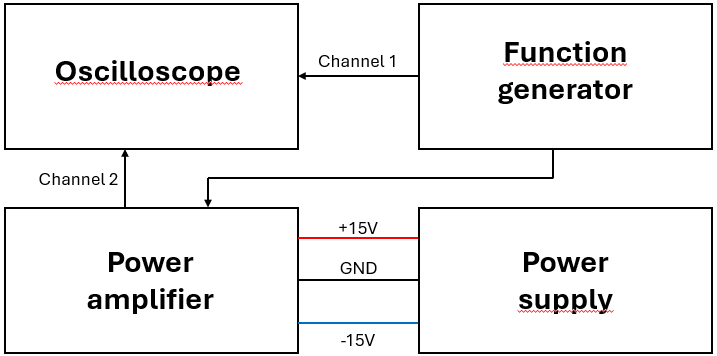
\includegraphics[width=0.8\linewidth]{TU Delft Booming Bass Project Report/figures/test setup.png}
    \caption{A schematic of the measuring setup used to analyze the performance of the power amplifier}
    \label{fig:PA test setup}
\end{figure}
%\begin{figure}[H]
%\centering
%\resizebox{0.75\textwidth}{!}{%
%\begin{circuitikz}
%\tikzstyle{every node}=[font=\Large]
%\draw  (2.75,18) rectangle (7,15.75);
%\draw  (10.5,18) rectangle (15,15.75);
%\draw  (2.75,14.25) rectangle (7,11.75);
%\draw  (10.5,14.25) rectangle (15,11.75);
%\draw [->, >=Stealth] (10.5,16.75) -- (7,16.75);
%\draw [->, >=Stealth] (5,14.25) -- (5,15.75);
%\draw [->, >=Stealth] (10.5,13) -- (7,13);
%\draw [->, >=Stealth] (10.5,13.75) -- (7,13.75);
%\draw [->, >=Stealth] (10.5,12.25) -- (7,12.25);
%\draw [short] (11.75,15.75) -- (11.75,15);
%\draw [short] (11.75,15) -- (6,15);
%\draw [->, >=Stealth] (6,15) -- (6,14.25);
%\end{circuitikz}
%}%
%\caption{a schematic of the measuring setup used to analyze the performance of the power amplifier}
%\label{fig:test setup}
%\end{figure}

The measurement procedure for the power amplifier circuit consisted of the following steps:
\begin{enumerate}
\item The input signal $\mathbf{V_{in}}$ from the Tektronix AFG 3021B/C function generator was connected at varying frequencies.
\item Both the input $\mathbf{V_{in}}$ and output $\mathbf{V_{out}}$ voltages were measured using the Tektronix TDS 2022B oscilloscope.
\item The gain was calculated by dividing the output voltage $\mathbf{V_{out}}$ by the input voltage $\mathbf{V_{in}}$.
\item The results from step 3 was then applied to \seautoref{eq: V to db}.

\end{enumerate}
 


\begin{figure}[h]
    \centering
    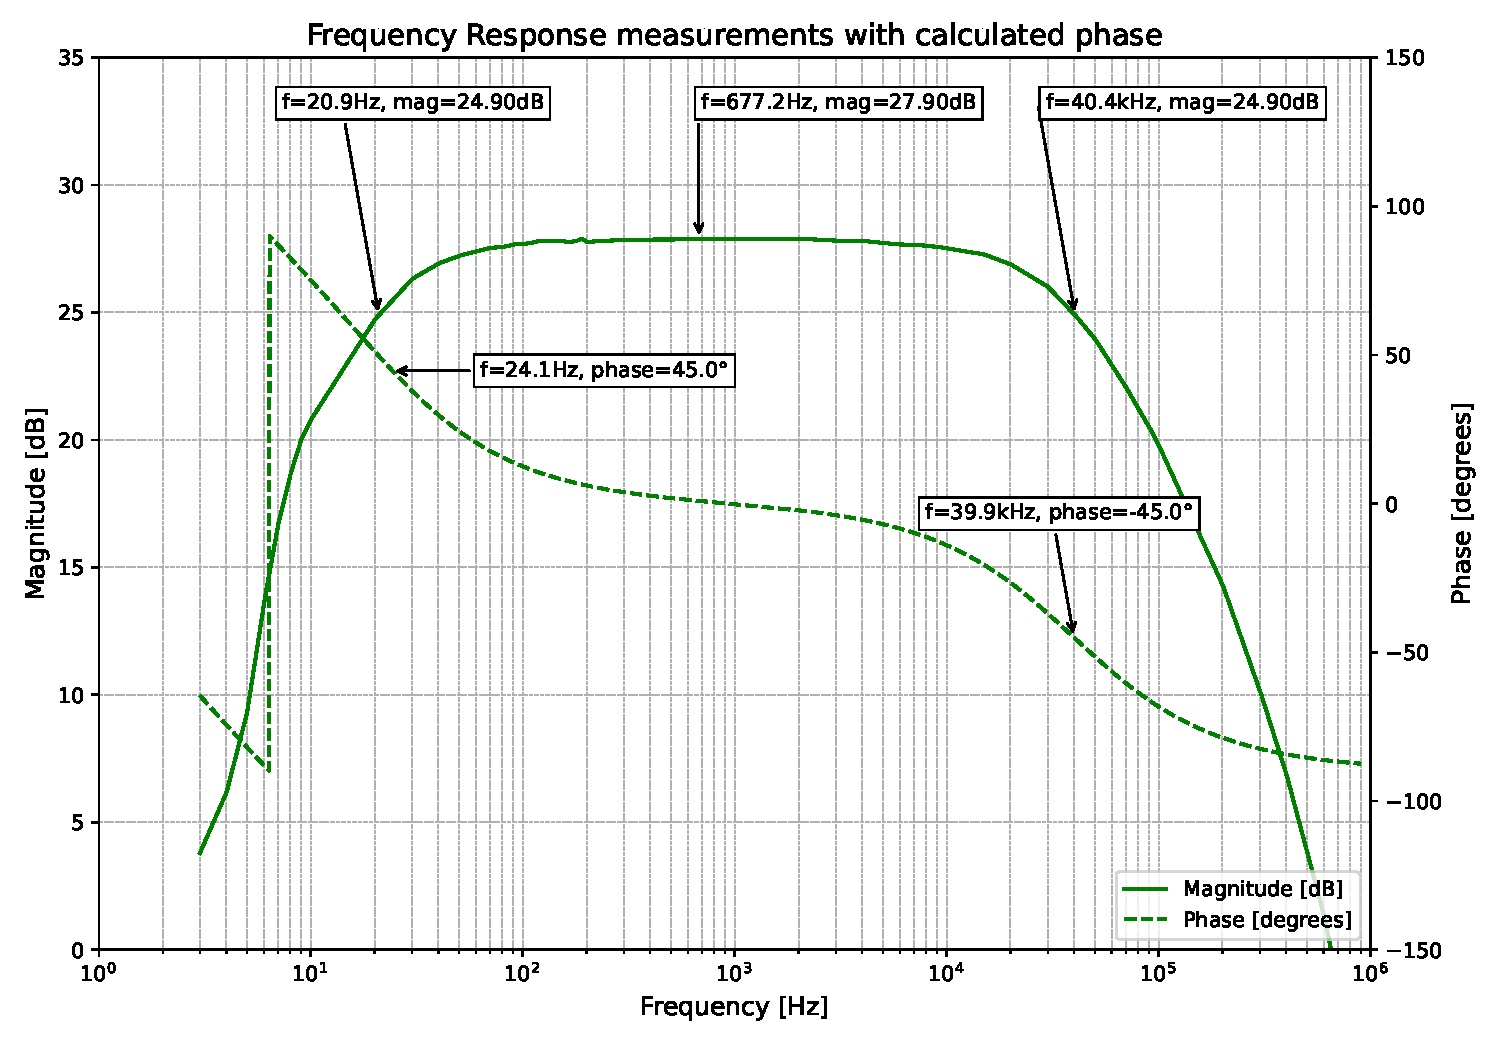
\includegraphics[width=0.9\linewidth]{TU Delft Booming Bass Project Report/figures/PowerAmplifier/measurements/metingen met misschien goede phase.pdf}
    \caption{Bode plot of measurements made with the power amplifier circuit of B2-1}
    \label{fig:freq response with phase}
\end{figure}

\subsubsection{B2-1 Final Results}

When examining, for example, \autoref{fig:40kHz}, the mean value of the sinusoidal voltage can be observed. In channel 1 (which represents the signal directly from the function generator), this mean value is approximately 500mV, while in channel 2 (the signal output from the power amplifier), the mean value is around 300mV. All of the measurements are summarized in \stautoref{tab:measurement_results}. To convert the measurement data into a continuous graph, MatplotLib was employed. The data points were transformed into a logarithmic scale to extrapolate 2000 entry points, which were then converted back into a linear scale. This process resulted in the graph shown in \sfautoref{fig:freq response with phase}.

\subsubsection{Obtaining the phase}
As demonstrated in \autoref{fig:20Hz} and \autoref{fig:40kHz}, a phase shift is observed between the output of the power amplifier and the function generator. Both signals are approximately in phase around 1kHz (see \sfautoref{fig:900Hz 400}). Plotting this phase shift based on the measurements proved to be difficult, so a function was created for use in Python to simplify the calculations (refer to \shortautoref{calculation of phase} for the code). This can be accomplished using \seautoref{eq: total transfer} (for the complete derivation of the phase equation, see \shortautoref{sec: phase calc}). The final phase plot is shown in \sfautoref{fig:freq response with phase}.

% In \sfautoref{fig:20Hz} and \sfautoref{fig:40kHz} two measurements can be seen, with a phase shift. Channel 1(the orange sinusoid) is from the function generator and channel 2 (the blue sinusoid) is the output of the power amplifier. An extra measurement where the phase is roughly the same between channel 1 and channel 2 can be seen in \sfautoref{fig:900Hz 400}


\begin{figure}[H]
\centering
\captionsetup{justification=raggedright, labelfont=bf}
\begin{subfigure}{.5\textwidth}
  \centering
    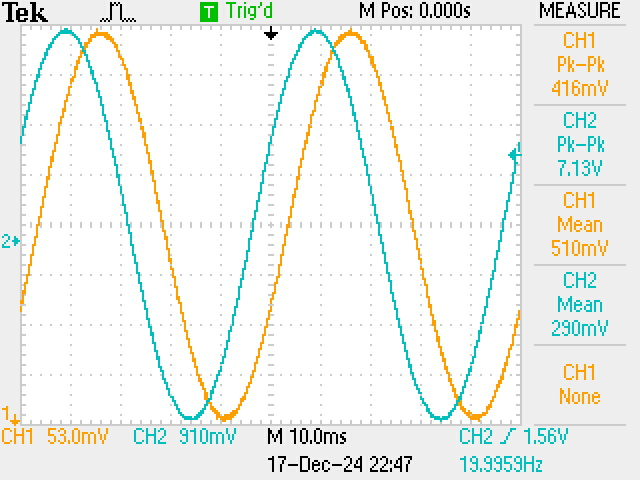
\includegraphics[width=0.95\linewidth]{TU Delft Booming Bass Project Report/figures/PowerAmplifier/measurements/20Hz.JPG}
    \captionsetup{justification=raggedright, labelfont=bf}
    \caption{A measurement with output from a function generator and the power amplifier at 20Hz.}
    \label{fig:20Hz}
\end{subfigure}%
\begin{subfigure}{.5\textwidth}
  \centering
    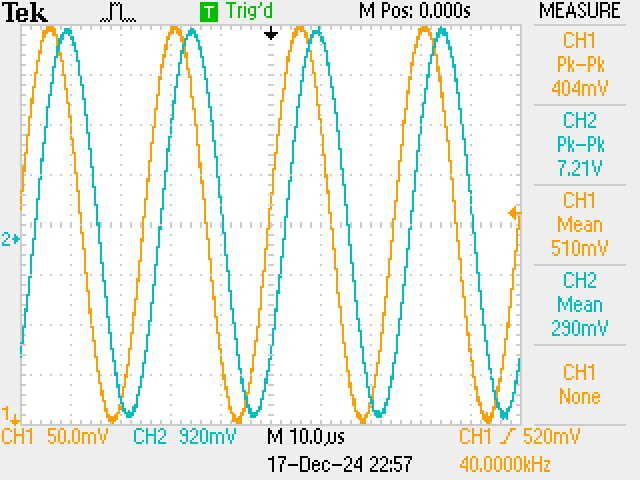
\includegraphics[width=0.95\linewidth]{TU Delft Booming Bass Project Report/figures/PowerAmplifier/measurements/40kHz.JPG}
    \captionsetup{justification=raggedright, labelfont=bf}
    \caption{A measurement with output from a function generator and the power amplifier at 40kHz.}
    \label{fig:40kHz}
\end{subfigure}
\caption{Two measurements showing the output of the function generator and B2-1's power amplifier at \~ 400mV, a clear phase shift is visible.}




\end{figure}

\begin{table}[H] % Ensures the table stays in place
\centering
\caption{Measurement Results from 3Hz to 900kHz of B2\_1's power amplifier}
\label{tab:measurement_results}
\begin{tabular}{|c|c||c|c||c|c|}
\hline
freq (Hz) & magnitude (dB) & freq (Hz) & magnitude (dB) & freq (Hz) & magnitude (dB) \\\hline
3 & 3.793281 & 150 & 27.809591 & 9000 & 27.576474 \\\hline
4 & 6.155268 & 160 & 27.767426 & 10000 & 27.515459 \\\hline
5 & 9.285681 & 170 & 27.767426 & 15000 & 27.276017 \\\hline
6 & 13.547177 & 180 & 27.809591 & 20000 & 26.890415 \\\hline
7 & 16.645216 & 190 & 27.895167 & 30000 & 26.010078 \\\hline
8 & 18.632909 & 200 & 27.767426 & 40000 & 24.936278 \\\hline
9 & 20.000000 & 300 & 27.853002 & 50000 & 23.974499 \\\hline
10 & 20.780155 & 400 & 27.853002 & 60000 & 22.937866 \\\hline
20 & 24.713002 & 500 & 27.853002 & 70000 & 22.079298 \\\hline
30 & 26.308784 & 600 & 27.895167 & 80000 & 21.255817 \\\hline
40 & 26.918908 & 700 & 27.895167 & 90000 & 20.525305 \\\hline
50 & 27.218201 & 800 & 27.895167 & 100000 & 19.803824 \\\hline
60 & 27.389528 & 900 & 27.895167 & 200000 & 14.341809 \\\hline
70 & 27.532069 & 1000 & 27.895167 & 300000 & 10.192336 \\\hline
80 & 27.557118 & 2000 & 27.895167 & 400000 & 6.915987 \\\hline
90 & 27.663610 & 3000 & 27.809591 & 500000 & 3.907928 \\\hline
100 & 27.681000 & 4000 & 27.809591 & 600000 & 1.413815 \\\hline
110 & 27.723164 & 5000 & 27.723164 & 700000 & -1.280346 \\\hline
120 & 27.809591 & 6000 & 27.662902 & 800000 & -3.262526 \\\hline
130 & 27.809591 & 7000 & 27.662902 & 900000 & -5.171004 \\\hline
140 & 27.809591 & 8000 & 27.618133 &  &  \\\hline
\end{tabular}
\end{table}

\subsubsection{B2-2 Final Design Results}

Some of the measurements of B2-2's power amplifier can be seen in \sfautoref{B2-2 PA measurements} and \sfautoref{fig:B2-2 3kHz}. The cut-off frequencies are at around 19.5Hz and 34kHz and the maximum voltage gain is about 26.6, or 28.5dB.
\begin{figure}[H]
\centering

\begin{subfigure}{.5\textwidth}
  \centering
    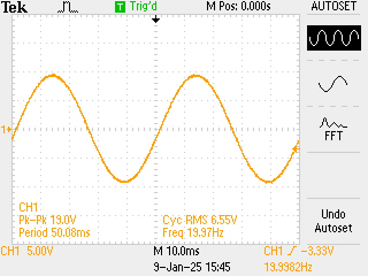
\includegraphics[width=0.95\linewidth]{TU Delft Booming Bass Project Report/figures/PowerAmplifier/measurements/Afbeelding1.png}
    \captionsetup{justification=raggedright, labelfont=bf}
    \caption{B2-2's measurement with output from the power amplifier at 20Hz.}
    \label{fig:B2-2 20Hz}
\end{subfigure}%
\begin{subfigure}{.5\textwidth}
  \centering
    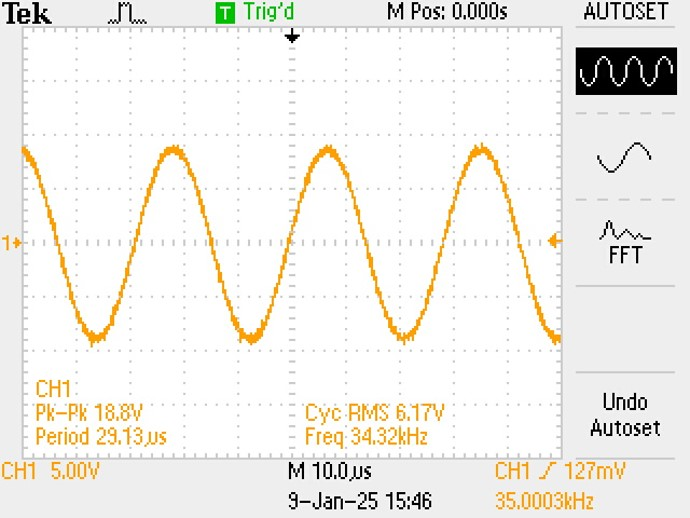
\includegraphics[width=0.95\linewidth]{TU Delft Booming Bass Project Report/figures/PowerAmplifier/measurements/Afbeelding2.jpg}
    \captionsetup{justification=raggedright, labelfont=bf}
    \caption{B2-2's measurement with output from the power amplifier at 35kHz.}
    \label{fig:B2-2 35kHz}
\end{subfigure}%
\captionsetup{justification=raggedright, labelfont=bf}
\caption{Two measurements showing the output of B2-2's power amplifier at 1V from the function generator.}
\label{B2-2 PA measurements}
\end{figure}

\subsubsection{Measurement at maximum gain}
\begin{figure}[H]
    \captionsetup{justification=raggedright, labelfont=bf}

\begin{subfigure}[t]{0.5\linewidth}
    \centering
    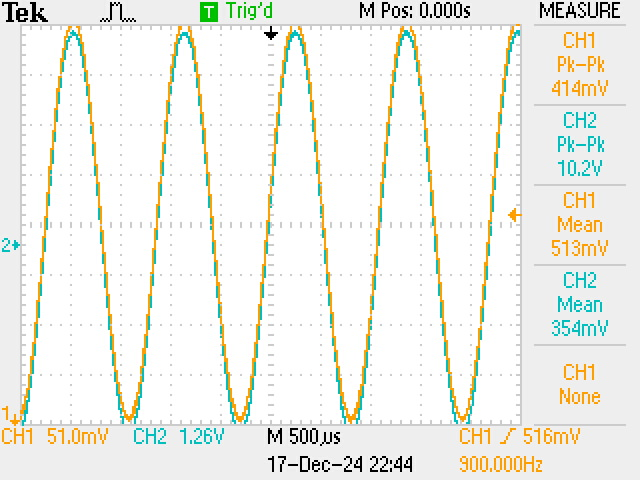
\includegraphics[width=0.9\linewidth]{TU Delft Booming Bass Project Report/figures/PowerAmplifier/measurements/900Hz.JPG}
    \caption{A measurement showing the output of the function generator and B2-1's power amplifier at \textasciitilde 400mV and 900Hz. Where the function generator and the power amplifier are almost in phase}
    \label{fig:900Hz 400}

\end{subfigure}
\begin{subfigure}[t]{0.5\linewidth}

  \centering
    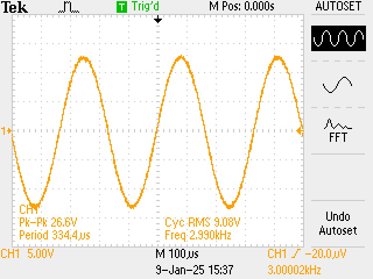
\includegraphics[width=0.9\linewidth]{TU Delft Booming Bass Project Report/figures/PowerAmplifier/measurements/Afbeelding3.png}
    \caption{B2-2's measurement with output from the power amplifier at 3kHz with 1V from the function generator.}
    \label{fig:B2-2 3kHz}

\captionsetup{justification=raggedright, labelfont=bf}
\label{B2 PA measurements 2}
\end{subfigure}
\caption{Two extra measurements of B2-1 and B2-2 power amplifier at around the maximum gain}

\end{figure}

\subsection{Filters}
The measurements serve as the key benchmark for evaluating the filter's quality. These measurements were collected throughout the filter design process, allowing for iterative adjustments. Ultimately, the final measurements included both acoustic and electric responses of the filters.

The acoustic measurements refer to the frequency-dependent response of the filter, which evaluates the power (in dB) of the acoustic signal emitted by the filter. On the other hand, the electric response involves analyzing the behavior of the filter across various frequencies, measured in terms of voltage gain (in dB).
\begin{figure}[H]
    \centering
    \begin{subfigure}[t]{0.48\textwidth}
        \centering
        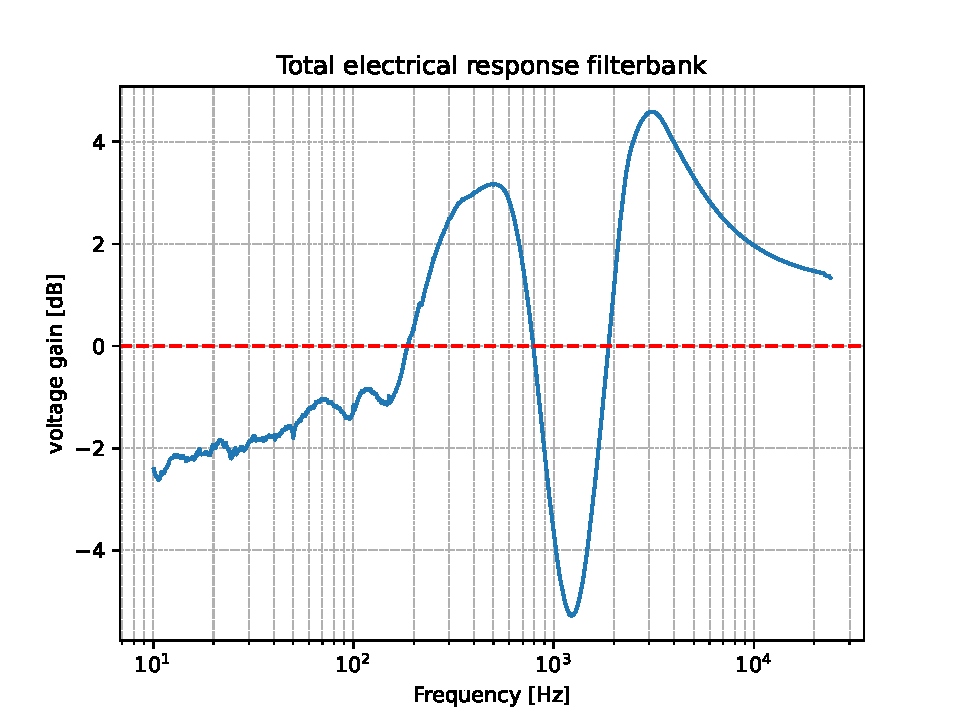
\includegraphics[width=\textwidth]{TU Delft Booming Bass Project Report/figures/FilterGroup/total_electric_response.pdf}
        \caption{The electric response of the filters.}
        \label{fig:electric_response}
    \end{subfigure}
    \hfill
    \begin{subfigure}[t]{0.48\textwidth}
        \centering
        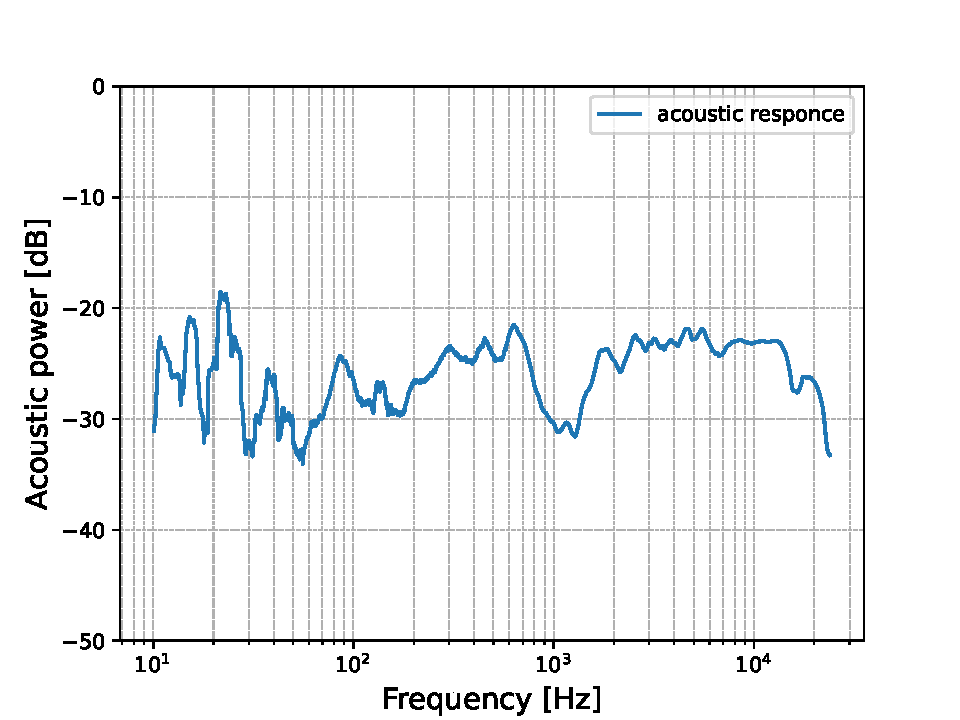
\includegraphics[width=\textwidth]{TU Delft Booming Bass Project Report/figures/FilterGroup/acoustic_response.pdf}
        \caption{The acoustic response of the filters shown at a 1-meter distance.}
        \label{fig:frequency_response}
    \end{subfigure}
    \captionsetup{justification=raggedright, labelfont=bf}
    \caption{A comparison of the electric and acoustic responses of the filters: (a) The electric response of the filters is depicted, showing the variations in the voltage gain across different frequencies. Significant changes in gain are observed, particularly at key frequency ranges, which could influence the overall performance of the system. (b) The acoustic response of the filters is shown at a 1-meter distance, illustrating how the system performs in terms of sound output and quality at this specific range.}
    \label{fig:combined_response}
\end{figure}

As observed in \sfautoref{fig:combined_response}, the electric response of the filters displays some inconsistencies. Notable gains occur around 500Hz and 1100Hz, while a dip in the voltage gain is evident between 800Hz and 1000Hz. This fluctuation may potentially impact the accuracy of the acoustic response, as it suggests a not-flat frequency response. Despite this, the acoustic response remains relatively flat, with fluctuations of approximately 10dB at max at around 1kHz. This deviation is directly attributed to the significant dip in the electric response seen in \sfautoref{fig:electric_response}. Furthermore, the decrease in acoustic power at this frequency range can be anticipated from the mid-band acoustic amplitude response in \sfautoref{fig: Cutoff frequencies}, where a similar reduction at 1000Hz aligns with both the electric and acoustic responses.

For the remained of the frequency range, the acoustic power remains relatively flat, with only minor dips and peaks. These slight variations are unlikely to significantly impact the overall sound quality of accuracy. Consequently, it can be concluded that the filters effectively contribute to the amplifier's ability to produce a more accurate and consistent sound profile.

\chapter{Discussion}
\label{chapter:discussion}
\section{Discussion}

\subsection{Power Supply}
\label{subsec:psdiscussion}
In this section a comparison is made between the simulated characteristics of the power supply and the measured results: where $D_{V_\text{Av}}$[\%], $D_{I_\text{res}}$[\%], and $D_{u_\text{ripple}}$[\%] correspond to the deviation between the simulated and measured results:
\begin{figure}[H]
    \centering
    \begin{minipage}{0.48\textwidth}
        \centering
        \captionsetup{justification=raggedright, labelfont=bf}
        \caption{Characteristics of the power supply in real-world applications under various load levels, using load resistors equipped with large heat sinks to dissipate the thermal energy from imperfect energy conversion. The data includes each load's average output voltage, current, and ripple percentage.}
        \begin{threeparttable}
          \centering
          
          \begin{tabular}{c @{\hspace{12pt}} *4{c} S @{\hspace{12pt}}}
            \toprule
            \multicolumn{5}{c}{\textbf{Deviation Power Supply Characteristic}} \\
            \cmidrule(lr){1-5}
            & & \multicolumn{3}{c}{\textbf{Deviations Performance Metr.}} \\
            \cmidrule(lr){3-5}
            & $R_\text{Load}$ [$\Omega$] & ${D_{V_\text{Av}}}$ [\%] & ${D_{I_\text{res}}}$ [\%] & ${D_{u_\text{ripple}}}$ [\%] \\
            \midrule
            1 & 19 & 9.84 & 10.08 & 25.19 \\
            2 & 38 & 7.65 & 8.53 & 16.08 \\
            3 & 76 & 6.83 & 7.41 & 41.03 \\
            4 & Open & 3.14 & - & -52.73 \\
            \bottomrule
          \end{tabular}
        \end{threeparttable}
        
        \label{tab:CharacteristicsSim}
    \end{minipage}\hfill
    \begin{minipage}{0.48\textwidth}
        \centering
        \resizebox{\linewidth}{!}{%
            \begin{tikzpicture} 
                \pgfplotsset{
                    every axis legend/.append style={at={(0.02,0.98)}, anchor=north west, legend columns = 1}, 
                    every axis/.append style={ytick distance=0.5, xtick distance=2, minor tick num=1, grid=major,
                    every axis grid/.append style={line width=0.5pt, draw opacity=0.4}}}
                \begin{axis} [xlabel = {Delivered power [W]}, ylabel = {Ripple [\%]}]
                 % First data set
                \addplot+[no markers, blue] table[row sep=crcr] 
                {
                    Supplied power(W):       Ripple(\%): \\  
                    21.31       3.23  \\
                    11.82     1.66  \\
                    6.351     1.10  \\
                    0     0.26  \\
                };
                \addlegendentry{Ripple [\%] - Measured}
                    \addplot+[no markers, red, dashed] table[row sep=crcr] {
                        Supplied Power (W):       Ripple(\%): \\  
                        17.63       2.58  \\
                        10.11     1.43  \\
                        5.54     0.78  \\
                        0     0.55  \\
                    };
                    \addlegendentry{Ripple [\%] - Simulated}
                \end{axis}
            \end{tikzpicture}%
        }
        \captionsetup{justification=raggedright, labelfont=bf}
        \caption{The output voltage ripple as a function of the power delivered to varying load resistances, showing the voltage ripple magnitude and the corresponding load power.}
        \label{fig:OutputVoltageRipplePower}
    \end{minipage}
\end{figure}

It can be seen that the difference between the simulated ripple voltage and the measured voltage is minimal. The same holds for the voltage and current values. This deviation can be caused by the physical characteristics of the smoothing capacitors and resistors. These components can have a deviation in their values, which can influence the output values. This does not cause great problems as all the requirements are still met. For future designs, it is therefore still recommended to use the same components.

As can be seen by comparing the simulation and measurement results in Fig. \ref{fig:OutputVoltageRipplePower}, it is clear that there is a significant discrepancy between them. This can be attributed to various factors:
\begin{itemize}
    \item The diodes used in the simulation differ from those used in reality. The 1N4148 diodes used in the simulation are general and are not fitted to carry large currents \cite{1n4148}. The 1N5408, on the contrary, can carry average rectified currents up to 3.0 A \cite{1n5408}. Therefore, the 1N5408 will result in much less loss over the diode.
    \item The transformer (CT-T) output voltage used in the simulation was set to 17${V_{\text{rms}}}$, whereas the measured output voltage was slightly higher at 17.25${V_\text{rms}}$. This small increase in voltage introduces a minor error in the simulated results, as the higher voltage directly affects the performance of the circuit.
    \item In the simulation, a 10mH inductor was used in series with the voltage source to simulate the transformer's impedance (CT-T's impedance). While this approach is reasonable, the real transformer's characteristics may slightly differ, leading to a small error and deviation in the results from the simulation when compared to the measurements.
\end{itemize}

As shown in Fig. \ref{fig:OutputCurrenteWith-Without}, the inclusion of smoothing capacitors results in a significant spike in the current, often referred to as rush-in current. This surge can be attributed to the charging process of the capacitors when they are first connected to the circuit. While the smoothing capacitors effectively reduce the ripple percentage and improve the stability of the output voltage $V_{\text{out}}$, this high initial current could potentially damage other components in the circuit if not properly managed.

This observation underscores the importance of carefully selecting the capacitor size to strike a balance between reducing ripple and minimizing the rush-in current. Exceeding an upper limit for the capacitor size could lead to reliability issues for the circuit components, emphasizing the need for circuit protection measures such as inrush current limiters (ICL) or thermistors (NTC, PTC) in future designs. 

\subsubsection{Future recommendations:}
Recoonmendations for improving the methodologies of the Power Supply subgroups include:
\begin{itemize}
    \item Implement the right components in the simulation since different diodes were used in the simulations compared to the actual design.
    \item Measure the output voltage of the transformer and implement this in the simulation.
    \item Measure the impedance of the transformer and implement this in the simulation.
\end{itemize}


\subsection{Power Amplifier}

\subsubsection{Analysis of Results}

The results obtained from the project show that the designed power amplifier closely aligns with the intended specifications. The pass-band gain of 24.83 is close to the desired gain of 25. Similarly, the measured cutoff frequencies of 20.9 Hz and 40.4 kHz almost meet requirement 1. The deviations observed in both gain and frequency response are insignificant and do not affect the amplifier's practical performance. Furthermore, the DC offset at the output of the function generator gets amplified by less than 1, which meets requirement 3 mentioned earlier for the power amplifier circuit.

To illustrate these deviations, the table below compares the ideal, simulated, and measured values, along with percentage deviations:
\begin{table}[H]
    \centering
    \captionsetup{justification=raggedright, labelfont=bf}
    \caption{Comparison of required, simulated, and measured values and deviations between the parameters for B2-1's power amplifier circuit. The deviation D$_{\text{diff},1}$ represents the difference between the simulated and required values, while D$_{\text{diff},2}$ corresponds to the difference between the measured and required values.}
    \resizebox{\textwidth}{!}{
    \begin{tabular}{c @{\hspace{12pt}} *7{c} S @{\hspace{12pt}}}
        \toprule
        \multicolumn{7}{c}{\textbf{Comparison Table for B2-1 Power Amplifier Performance}} \\
        \cmidrule(lr){1-7}
       
        & Parameter & Calculated Value & Simulated Value & Measured Value & D$_{\text{diff},1}$ [\%] & D$_{\text{diff},2}$ [\%]  \\
        \midrule
        Lower Cut-off & $f_\text{cut-off}$ [Hz] & 20.0Hz & 20.1Hz & 20.9Hz & 0.50\% &  4.50\% \\
         \vspace{10pt} \\
        Upper Cut-off & $f_\text{cut-off}$ [Hz] & 40.0kHz & 40.3kHz & 40.4kHz & 0.75\% & 1.00\% \\
         \vspace{10pt} \\
        Pass-band voltage gain &  $G_{\text{Gain}}$ & 25.0 & 24.60 & 24.83 & -1.60\% & -0.68\%  \\
        
        
        \bottomrule
    \end{tabular}
    }
\end{table}

The alternate power amplifier design was also assessed, achieving a gain of 26.6 with cut-off frequencies at 20Hz and 34kHz. The table below compares these values to those of the chosen amplifier and the specified requirements, including the percentage deviations:
\begin{table}[H]
    \centering
    \captionsetup{justification=raggedright, labelfont=bf}
    \caption{Comparison of required, simulated, and measured values and deviations between the parameters for B2-2's power amplifier circuit. The deviation D$_{\text{diff},1}$ represents the difference between the simulated and required values, while D$_{\text{diff},2}$ corresponds to the difference between the measured and required values.}
    \resizebox{\textwidth}{!}{
    \begin{tabular}{c @{\hspace{12pt}} *7{c} S @{\hspace{12pt}}}
        \toprule
        \multicolumn{7}{c}{\textbf{Comparison Table for B2-1 Power Amplifier Performance}} \\
        \cmidrule(lr){1-7}
       
        & Parameter & Calculated Value & Simulated Value & Measured Value & D$_{\text{diff},1}$ [\%] & D$_{\text{diff},2}$ [\%]  \\
        \midrule
        Lower Cut-off & $f_\text{cut-off}$ [Hz] & 20.0 Hz & 20.4 Hz & 19.5 Hz & 2.00\% & -2.56\% \\
         \vspace{10pt}\\
        Upper Cut-off & $f_\text{cut-off}$ [Hz] & 40.0 kHz & 40.0 kHz & 34.0 kHz & 0.00\% & -15.00\% \\
         \vspace{10pt}\\
        Pass-band voltage gain & $G_{\text{Gain}}$ & 25.0 & 24.90 & 26.60 & -0.40\% & -5.60\%  \\
        
        
        \bottomrule
    \end{tabular}
    }
\end{table}

The small deviations observed between the simulated and measured results in the above two tables can be attributed to several factors:
\begin{enumerate}
    \item \textbf{Component Tolerances:} Real-world resistors and capacitors exhibit variations of up to 20\% from their nominal values, affecting the frequency response and gain. These variations result in slight discrepancies between the measured and simulated results.
    \item \textbf{Non-Ideal Op-Amps:} The LM3886 op-amp exhibits non-ideal characteristics, including input offset voltage and a finite gain-bandwidth product, which cause discrepancies from ideal calculations.
    \item \textbf{Soldering and Connections:} Small resistances or imperfect connections during soldering may have slightly altered the circuit's behavior, leading to deviations from the expected performance.
\end{enumerate}

\subsubsection{Final Circuit Choice}
Will all the information gathered, it is now possible to select the power amplifier to be used in the final loudspeaker system. To make this decision, both systems are compared against the requirements outlined in Sec. \ref{requirements PA}:

 
\label{section: choosing a circuit}
\begin{itemize}[H]
    \item \textbf{Requirement 1:} The lower cut-off frequency of B2-1's amplifier is 20.9Hz, which is slightly father from the desired 20Hz compared to B2-2's amplifier, which achieved a cut-off frequency of 19.5Hz. However, the upper cut-off frequency of B2-1's amplifier is 40.4kHz, which is closer to the desired value than B2-2's cut-off of 34.4kHz.
    \item \textbf{Requirement 2:} The gain of B2-1's power amplifier ended up at 24.83, while B2-2's circuit reached a gain of 26.6. Therefore B2-1's power amplifier circuit is closer to the desired and required factor of 25 voltage gain and is less likely to cause speaker clipping at certain frequencies.
    \item\textbf{Requirement 3:} There was no significant difference between the two amplifier circuits in terms of the amount of DC offset eliminated.
\end{itemize}
After evaluating these three key requirements, the decision was made to use B2-1's power amplifier in the final system. Two out of the three requirements were much closer to the desired values in B2-1 compared to B2-2. The deviations in B2-1's power amplifier do not affect its ability to amplify the correct frequencies at the proper rate; These results demonstrate that the design approach was effective, and the chosen amplifier performs as expected, making it suitable for the required real-world applications.

\subsubsection{Phase}
The kink (abrupt change) observed in the phase response \autoref{fig:freq response with phase} remains unexplained. Despite thoroughly reviewing the derivations, no mistakes were found. Additionally, the discrepancy between the phase calculated using Python and the phase calculated by LTSpice is likely due to the different methods each tool uses to calculate the phase. While it is difficult to definitively determine which method yields a more accurate result, the Python-calculated phase has a higher likelihood of being close to the correct answer, as the phase should not reach values of 150 or -150 degrees at any point in the graph (see \autoref{fig:real circuit results}). However, since the measurements in \sfautoref{fig:freq response with phase} match the simulations closely, the phase shown in the same graph is likely to closely match the phase if it were measured.






\newpage
\subsection{Loudspeaker and Filters}
\subsubsection{Loudspeaker Models}
While the loudspeaker model aligns with the physical circuit's general shape and impedance frequency behavior, some discrepancies remain. The most notable is the reduced accuracy of the tweeter's model compared to the other speaker models. This could likely be because the model is better suited for speakers with lower resonant frequencies. Additionally, at frequencies below and above the resonance peak, the model tends to underestimate the total impedance $Z_{\text{tot}}$ of all three speakers, with the tweeter experiencing the greatest deviation.

However, the model performs very well in predicting the impedance behavior around the resonance peaks, which is the critical frequency range where the speaker operates most effectively. This accurate representation of the resonance frequencies ensures the model remains valuable for its primary purpose.

\subsubsection{Filters}
The design methodology was effectively implemented, enabling the filters to be built on time and allowing sufficient opportunity for evaluation. While there was room for improving efficiency through better communication between the three groups, the overall process was carried out in a well-structured manner.

Simulations conducted using LTSpice played a critical role in the filter development process, providing the group with a means to verify their design and refine their understanding. As shown in \sfautoref{fig:freq_resp}, the resulting frequency response is not entirely flat, exhibiting a maximum deviation of 5.0dB at approximately 510Hz. This deviation was deemed acceptable, as further adjustments to component values shifted the cut-off frequency into less favorable ranges, compromising the overall performance of the filter.

The insights gained from these simulations enabled thoughtful refinement of the filters. However, the reliance on simulations may have been excessive. While real-world testing was conducted, incorporating more frequent hands-on testing could have provided additional practical validation and potentially expedited optimization.

Measurements confirmed the effectiveness of the chosen methodology. As shown in \sfautoref{fig:electric_response}, the electric frequency response of the three combined possible filters aligns well with the corresponding simulations. The maximum observed deviation is approximately 5.2dB at around 1000Hz, which is acceptable since further tuning resulted in undesirable shifts in cut-off frequencies.

This behavior aligns with the simulations shown in \sfautoref{fig:freq_resp}, where a similar dip of approximately 4.5dB is observed near 100Hz. Analysis of the simulation indicates that this dip coincides with a phase shift from -180$^{\circ}$ to +180$^{\circ}$, causing signal deconstructive interference at this frequency. The differences between measurements and simulations are minor and can be attributed to the use of real components, which inherently deviate slightly from their ideal values, leading to small measurement discrepancies.

The chosen and the alternate filter responses were then compared. The acoustic response of both aggregated filters, measured at a distance of 1 meter, is shown in \sfautoref{fig:combined_response_with_alternate} 
\begin{figure}[H]
    \centering
    \begin{subfigure}[t]{0.48\textwidth}
        \centering
        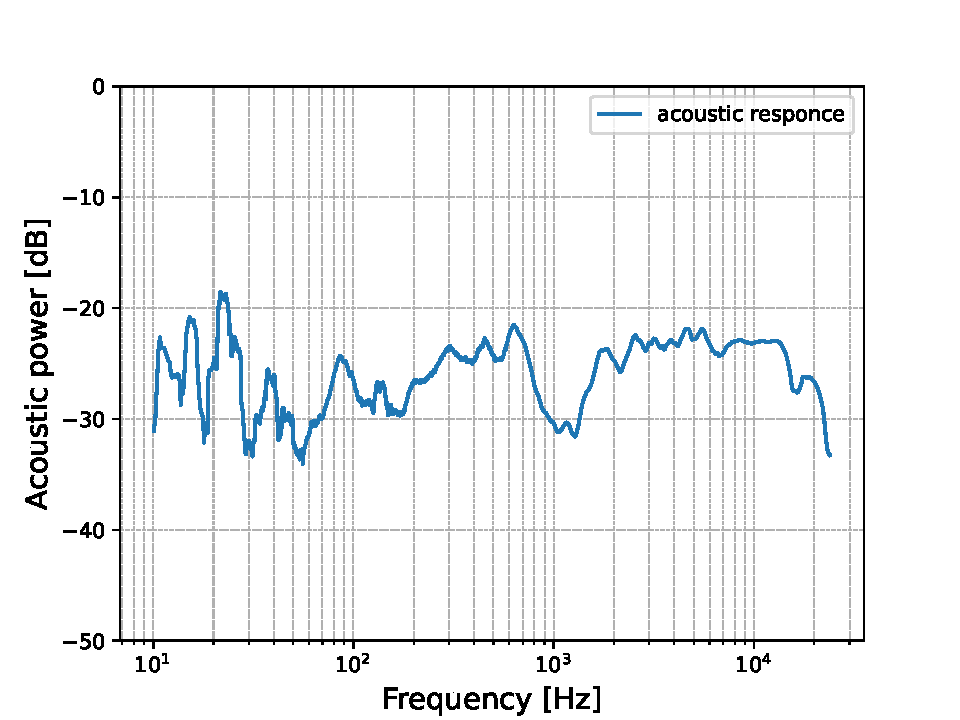
\includegraphics[width=\textwidth]{TU Delft Booming Bass Project Report/figures/FilterGroup/acoustic_response.pdf}
        \caption{The acoustic response of the chosen filter.}
        \label{fig:frequency_response}
    \end{subfigure}
    \hfill
     \begin{subfigure}[t]{0.48\textwidth}
         \centering
        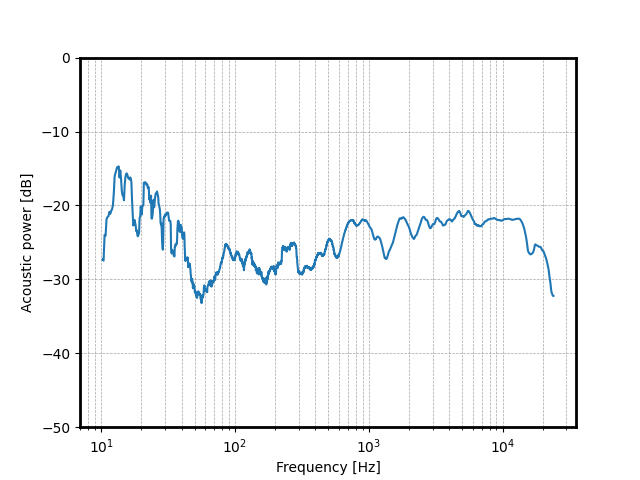
\includegraphics[width=\textwidth]{TU Delft Booming Bass Project Report/figures/FilterGroup/response_of_alternate_filterbank.png}
        \caption{The acoustic response of the alternate filter.}
        \label{fig:freq response alternate}
    \end{subfigure}
    
    \captionsetup{justification=raggedright, labelfont=bf}
    \caption{(L-R) Comparison between 2 filter banks: the chosen and alternate designs. The chosen filter exhibits a noticeably flatter acoustic response compared to the alternate filter.}
    \label{fig:combined_response_with_alternate}
\end{figure}

Both aggregated filters, each comprising their respective low-pass, band-pass, and high-pass filters, exhibit similar but slightly different acoustic power patterns. These differences primarily arise from variations in crossover frequencies and corresponding component values present in the filter circuits.

In the frequency range of 100Hz to 200Hz, the alternate filter demonstrates a higher maximum acoustic response compared to the chosen design. Additionally, the alternate design offers an advantage with a less pronounced dip in acoustic response between 1kHz and 2kHz. However, as the primary objective is to achieve the flattest frequency/acoustic response with the smallest maxima and largest minima, the response shown in \sfautoref{fig:frequency_response} for the chosen design remains the preferred option. 

\subsection{Future Recommendations}
The amplifier design process is long and involves many steps. It requires many parts to come together in an orderly fashion to create the amplifier successfully. While the three subgroups were able to create an amplifier that accurately recreated audio, adjustments to the methodology could have improved the design and construction of the components. 

For the design methodology, filter groups could have worked together more closely to find the component values for their filters. Currently, all three groups wrote different code and did their own Python simulations. By all using the same code, for example, they would have significantly reduced the time of the design process. Moreover, the filter groups could have done more tests in the real world of their filters, rather than relying on simulations in LT-Spice for adjusting the component values of the filters. It was highlighted that real-world tests gave the best insight into the quality of the filter. Therefore it would have been beneficial to the synthesis stage of the process.

Most of the steps taken in the design of the chosen power amplifier got quite accurate results. For that reason, the only future recommendation that could be made is to look again at the formula for the calculation of the phase in \ref{chapter:measurements}.  The derivation of this formula was gone over several times and a mistake was not found. So it would probably be beneficial to go over the transfer function again to see if somewhere along the line a mistake was made, or if perhaps the whole method of obtaining the function should be different by trying different ones. Furthermore a more accurate result for the phase shift could be obtained by measuring the phase at each frequency point chosen for measurements for this power amplifier.

\chapter{Conclusion}
\label{chapter:conclusion}
\section{Conclusion}
In conclusion, the sound amplifier was successfully designed and built by the team through a structured and methodical approach. Initially, each component was designed separately, supported by calculations and simulations to identify the theoretically optimal values. Once the design phase was complete, the team utilized available lab components to construct each system sub-component. Testing and adjustments were made to improve the performance of the sub-components if needed.

The final result is a well-integrated loudspeaker system capable of producing high-quality audio, as demonstrated by the frequency response in Fig. \ref{fig:frequency_response}. Additionally, the best-performing parts were selected for the final amplifier assembly. The overall audio output was further enhanced when connected to the Booming Bass (\cite{Linkwitz}) extension, achieving greater accuracy by introducing a flatter base.

The power supply group successfully built a fully operational power supply that met all required specifications and requirements. The output voltages were within the specified range, and the ripple voltage remained below 5\%, making it suitable for integration into the amplifier system. The power supply also fully discharges within the specified time of 150 seconds after being disconnected to ensure safe operation.

The power amplifier group also delivered a functional amplifier that met all performance requirements. The corner frequencies observed in the frequency response graph (see \autoref{fig:freq response with phase}) were 20.9Hz and 40.4kHz, with a gain of 27.90dB, demonstrating the amplifier's capability to operate effectively within the desired parameters.

The filter groups completed three distinct filters with cut-off frequencies at 150Hz for the low-pass filter and 1250Hz for the high-pass filter. This design ensures a balanced input to the speaker, contributing to a flat frequency response, as shown in \autoref{fig:frequency_response}. While a maximum difference of 10dB in acoustic power was observed due to a drop in the filter bank's electrical response, this was not considered to be of significant concern.

Python and LT-Spice simulations played a crucial role throughout the project by providing valuable insights into component behavior, allowing the team to make informed decisions and adjustments to optimize the amplifier's performance.

Overall, the project objectives were successfully achieved, resulting in a high-quality end product.




%input{mainmatter/chapter-2}
%\chapter{Loudspeaker Analysis}
\label{chapter:LoudspeakerAnalysis}

\section{Introduction}
A speaker functions by converting electrical current into mechanical motion, thereby generating an acoustic signal. The current passing through the voice coil induces vibrations in the speaker cone, causing a difference in sound pressure and thus producing sound waves. The speaker's physical dimensions are crucial in shaping its response to electrical inputs. To design efficient filters, it is necessary to represent the speaker's behavior with an equivalent electrical circuit. This approach facilitates precise predictions of the speaker's response to different input signals. This chapter outlines the structure of the electrical model and the methodologies used to determine its parameters.

\subsection{Loudspeaker Specifications}
The objective is to determine the appropriate values for the capacitors, inductors, and resistors in the electrical equivalent circuit representing the physical loudspeakers. Once these component values are identified, the circuit will be simulated over the frequency range of 20Hz to 20kHz. The simulated behavior will then be compared with the measured frequency response of the loudspeakers, ensuring that any significant deviation and discrepancy between the measured and simulated responses remains minimal to ensure high efficiency and function as projected.

\section{Loudspeaker Circuit Models}
\subsection{Model at Resonant Frequency}
The behavior of the speakers can be represented by an equivalent circuit comprising resistors, capacitors, and inductors. The capacitors and inductors model the speaker's frequency-dependant characteristics. At certain frequencies, the speaker exhibits predominantly higher resistive behavior, primarily influenced by the natural resonant frequency of the speaker's cone. The circuit model consists of five elements arranged as shown in Fig. \ref{fig:impedance_model1}. Here, $R_e$ represents the impedance at DC conditions, $L_e$ models the inductance of the voice coil, and the parallel RLC branch represents the mechanical properties of the cone. In this parallel branch, $R_p$ corresponds to frictional losses, $L_p$ models the mass of the cone, and $C_p$ represents its spring-like behavior \cite{johnshopkins_rlc}.
\begin{figure}[H]
    \centering
    \captionsetup{justification=raggedright, labelfont=bf}
    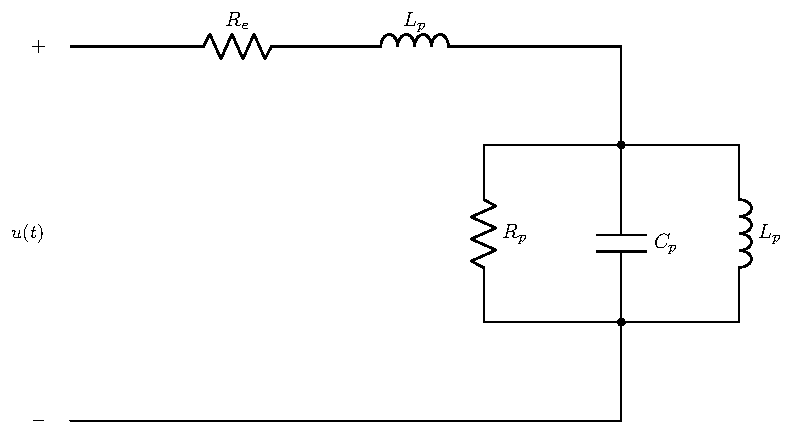
\includegraphics[width=0.6\linewidth]{figures/FilterGroup/ImpedanceModel1.pdf}
    \caption{Impedance model of the loudspeakers, depicting the equivalent circuit configuration used to represent the speaker's electrical ($R_e$, $L_e$) and mechanical properties ($R_p$, $C_p$, $L_p$ )\cite{IP-manual}.}
    \label{fig:impedance_model1}  
\end{figure}

\subsection{Model above Resonant Frequency}
At frequencies above and significantly higher than the cone's resonant frequency, the equivalent circuit can be further simplified. The total impedance of the circuit could be calculated using Eq. \ref{eq:total impedance}. For $\omega \gg \omega_o$, where $\omega_o$ is the resonant frequency of the circuit, the parallel components $R_p, C_p$ and $L_p$ can be disregarded due to their diminished influence on the overall impedance. To justify this simplification, the analysis should employ a normalized angular frequency $\omega'$ defined as followed:
\begin{flalign}
    \label{eq:normalize frequency}
    \omega' = \frac{\omega}{\omega_o}
    \equnit{\si{\text{rad s^{-1}}}}
\end{flalign}
The total impedance of the loudspeaker model is given by
\begin{flalign}
    \label{eq:total impedance}
    Z_{tot} = R_e + j\omega L_e + \frac{1}{\frac{1}{R_p}+j\omega C_p+\frac{1}{j\omega L_p}}
    \equnit{\si{\Omega}}
\end{flalign}

By applying Eq. \ref{eq:normalize frequency} and substituting it into Eq. \ref{eq:total impedance}, a revised expression for the total impedance, $Z_{tot}$, is obtained, as presented in Eq. \ref{eq:normalized impedance}:
\begin{flalign}
    \label{eq:normalized impedance}
    Z_{tot} = R_e + j\frac{\omega'}{\sqrt{L_pC_p}}L_e + \frac{1}{\frac{1}{R_p}+j\sqrt{\frac{C_p}{L_p}}\left(\omega'-\frac{1}{\omega'}\right)}
    \equnit{\si{\Omega}}
\end{flalign}

%-----------------------------------------------------------

You can rewrite $\omega$ as $\omega'\omega_o$. We can substitute the expression from Eq~\ref{eq:resonant frequency appA} \cite{IP-manual} and we will end up with the final expression for $\omega$ as seen in Eq~\ref{eq:final omega appA}.

\begin{flalign}
    \label{eq:resonant frequency appA}
    \omega_o = \frac{1}{\sqrt{L_pC_p}}
    \equnit{\si{\text{rad s^{-1}}}}
\end{flalign}

\begin{flalign}
    \label{eq:final omega appA}
    \omega = \frac{\omega'}{\sqrt{L_pC_p}}
    \equnit{\si{\text{rad s^{-1}}}}
\end{flalign}

For the next part I would like to define $Z_{par}$ as the impedance of the parallel RCL part of the circuit (Eq~\ref{eq:parallel impedance appA}).
\begin{flalign}
    \label{eq:parallel impedance appA}
    Z_{par} = \frac{1}{\frac{1}{R_p}+j\omega C_p+\frac{1}{j\omega L_p}}
    \equnit{\si{\Omega}}
\end{flalign}

If we want have a look at what happens with $Z_{par}$ when $\omega >> \omega_o$, we could see what happens to the impedance when $\omega'>>1$. First we need to rewrite the equation in terms of $\omega'$:
\begin{flalign}
\label{eq:capacitive_impedance appA}
    j\omega C_p = j\omega'\sqrt{\frac{c_p}{L_p}}
    \equnit{\si{\Omega^{-1}}}
\end{flalign}
\begin{flalign}
\label{eq:inductive_impedance appA}
    \frac{1}{j\omega L_p} = -j\frac{1}{\omega'}\sqrt{\frac{C_p}{L_p}}
    \equnit{\si{\Omega^{-1}}}
\end{flalign}

Substituting Eq~\ref{eq:capacitive_impedance appA} and Eq~\ref{eq:inductive_impedance appA} into Eq~\ref{eq:parallel impedance appA} will result in Eq~\ref{eq:normalized impedance appA}.

\begin{flalign}
    \label{eq:normalized impedance appA}
    Z_{par} = \frac{1}{\frac{1}{R_p}+j\sqrt{\frac{C_p}{L_p}}(\omega'-\frac{1}{\omega'})}
    \equnit{\si{\Omega}}
\end{flalign}

Now we can observe that if $\omega'>>1$ then $Z_{par} << 1$. Because $Z_{tot} = R_e + j\omega L_p + Z_{par}$ we can say that if $\omega >> \omega_o$ then $Z_{tot} \approx R_e + j\omega L_p$.

%---------------------------------------------------------

The revised expression for $Z_{tot}$ corresponds to an equivalent circuit consisting of an inductor and a resistor, as shown in Fig \ref{fig:impedance_model2}. If the operating frequencies of the speaker are all significantly higher than the resonant frequency, utilizing this simplified model becomes more practical for analysis and design purposes.
\begin{figure}[H]
    \centering
    \captionsetup{justification=raggedright, labelfont=bf}
    \includegraphics[width=0.5\linewidth]{figures/FilterGroup/impedance_model2_speaker.jpg}
    \caption{Impedance model for frequencies above the resonant frequency, illustrating the simplified equivalent circuit consisting of an inductor $L_e$ and the resistor $R_e$ \cite{IP-manual}.}
    \label{fig:impedance_model2}
\end{figure}

\section{Calculate Model Parameters}
The determination of the five unknown parameters requires solving a set of five equations. By analyzing the circuit and its impedance, the necessary equations for parameter estimation can be derived. The measured impedance data is presented in Fig \ref{fig:abs_speakers}. Detailed derivations of these equations are provided in the IP-manual \cite{IP-manual}.
\begin{flalign}
    \label{eq:Re_model}
    R_e = \left. |Z| \right._{\omega=0}
    \equnit{\si{\Omega}}
\end{flalign}

where $R_e$ represents the equivalent resistance of the circuit under DC conditions, corresponding to the impedance when the frequency is zero ($\omega=0$). Similarly, the parallel resistance $R_p$ is derived by subtracting $R_e$ from the magnitude of the total impedance $|Z|$ at the resonant angular frequency denoted by $\omega= \omega_o$, as given in Eq. \ref{eq:Rp_model}:
\begin{flalign}
    \label{eq:Rp_model}
    R_p = \left. |Z| \right._{\omega=\omega_o} - R_e
    \equnit{\si{\Omega}}
\end{flalign}

where $R_p$ accounts for the frictional losses in the mechanical behavior of the speaker at resonance. The capacitance $C_p$, representing the spring behavior of the speaker cone, is related to $R_p$ by Eq. \ref{eq:Cp_model}:
\begin{flalign}
    \label{eq:Cp_model}
    C_p = \frac{1}{R_pB}
    \equnit{\si{F}}
\end{flalign}

where B characterizes the bandwidth of the speaker's cone. The inductance $L_p$, representing the mass of the speaker cone, is related to $C_p$ and the resonant angular frequency $\omega_o$ by Eq. \ref{eq:Cp_model}. 
The inductance $L_e$, which models the voice coil, can be derived from the impedance at high frequencies ($\omega \gg \omega_o$) using Eq \ref{eq:Le_model}:
\begin{flalign}
    \label{eq:Lp_model}
    L_p = \frac{1}{C_p\omega_o^2}
    \equnit{\si{H}}
\end{flalign}
\begin{flalign}
    \label{eq:Le_model}
    L_e = \frac{\sqrt{(|Z|_{\omega \gg \omega_o})^2-R_e^2}}{\omega}
    \equnit{\si{H}}
\end{flalign}

The next step involves solving the equations for the different speakers and simulating the models to compare their responses with the actual measured data. Tab.\ref{tab:speaker_components} presents the calculated component values.
\begin{figure}[H]
    \centering
    \begin{minipage}{0.5\textwidth}
        \centering
        \includegraphics[width=\linewidth]{TU Delft Booming Bass Project Report/figures/FilterGroup/abs_impedance_speakers .pdf}
        \captionsetup{justification=raggedright, labelfont=bf}
        \caption{Absolute value of the speaker impedance.}
        \label{fig:abs_speakers}
    \end{minipage}\hfill
    \begin{minipage}{0.5\textwidth}
        \centering
        \begin{threeparttable}
          \centering
          \begin{tabular}{c @{\hspace{12pt}} *4{c} S @{\hspace{12pt}}}
            \toprule
            \multicolumn{5}{c}{\textbf{Speaker Component Values}} \\
            \cmidrule(lr){1-5}
            & & \multicolumn{3}{c}{\textbf{Component Values}} \\
            \cmidrule(lr){3-5}
            & Component & Woofer & Tweeter & Midtoner \\
            \midrule
            1 & $R_e$ ($\Omega$) & 4.03 & 4.14 & 4.06 \\
            2 & $L_e$ (mH) & 0.182 & 0.247 & 0.053 \\
            3 & $R_p$ ($\Omega$) & 8.93 & 5.05 & 1.24 \\
            4 & $C_p$ (mF) & 1.31 & 1.75 & 0.14 \\
            5 & $L_p$ (mH) & 3.66 & 1.67 & 0.11 \\
            \bottomrule
          \end{tabular}
        \end{threeparttable}
        \captionsetup{justification=raggedright, labelfont=bf}
        \caption{Component Values for the woofer, tweeter, and mid-toner, showing each component's resistance, inductance, and capacitance values. The table highlights the different characteristics of the components used in the speaker system.}
        \label{tab:speaker_components}
    \end{minipage}
\end{figure}

\section{Model Transfer Function}
\subsection{Defining the Transfer Function}
The transfer function $H(\omega)$ of the system describes the behaviour of the system. It relates the input to the output of the system with the use of Eq. \ref{eq:transfer_function}, where $Y(\omega)$ is the output signal and $X(\omega)$ is the input signal. In the case of the loudspeaker analysis the input signal is the is the voltage $V(\omega)$ and the output signal is $I(\omega)$. The transfer function will represent the input impedance $Z(\omega)$ of the entire circuit. 

\begin{flalign}
    \label{eq:transfer_function}
    Y(\omega) = H(\omega)X(\omega)
\end{flalign}

\subsection{Calculation of the Transfer Function}
In our case the transfer function is the system impedance. So finding the transfer function is a matter of finding the equivalent impedance with the use of the basic calculation rules for parallel and series circuits. First we transform the circuit into the phasor domain as seen in Fig. \ref{fig:/model_phasor}. The total impedance is calculated with Eq. \ref{eq:total_impedance} where $Z_{par}$ resembles the impedance of the three parallel components and its value is calculated with Eq. \ref{eq:parallel_impedance}. combining the two equations results in Eq. \ref{eq:final_impedance}, which is the total transfer function.

\begin{flalign}
    \label{eq:total_impedance}
    Z(\omega) = R_e + j\omega L_e + Z_{par}
    \equnit{\si{\Omega}} 
\end{flalign}

\begin{flalign}
    \label{eq:parallel_impedance}
    Z_{par}(\omega) = \frac{L_pR_p\omega}{jC_pR_pL_p\omega^2+L_p\omega-jR_p}
    \equnit{\si{\Omega}} 
\end{flalign}

\begin{flalign}
    \label{eq:final_impedance}
    Z(\omega) = \frac{L_pR_p\omega + (L_e\omega+R_e)(jC_pR_pL_p\omega^2+L_p\omega-jR_p)}{jC_pR_pL_p\omega^2+L_p\omega-jR_p}
    \equnit{\si{\Omega}} 
\end{flalign}



\begin{figure}[H]
    \centering
    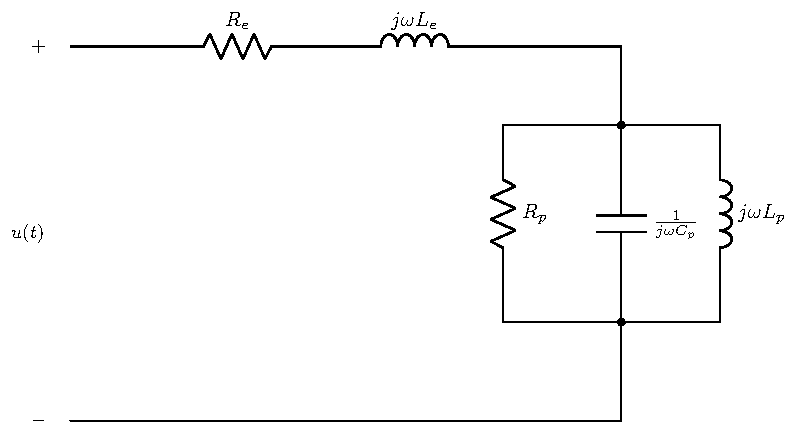
\includegraphics[width=0.4\textwidth]{TU Delft Booming Bass Project Report/figures/FilterGroup/impedance_model_phasor.pdf}
    \captionsetup{justification=raggedright, labelfont=bf}
    \caption{model circuit is phasor domain}
    \label{fig:/model_phasor}
\end{figure}


\section{Loudspeaker simulation}
Using the formulas derived from the circuit model, the corresponding component values can be found for each of the speakers. The calculations were done for each speaker by their respective filter group, which resulted in the component values found in Tab. \ref{tab:speaker_components}. 

Using the parameters found, the frequency response of each model was calculated and compared with the measured speaker data. This showed that the model matched closely around the resonance peak, but that the model generally had a slightly lower impedance than the measured data had as seen in Fig.\ref{fig:/model vs measured impedance}. 

\begin{figure}[H]
    \centering
    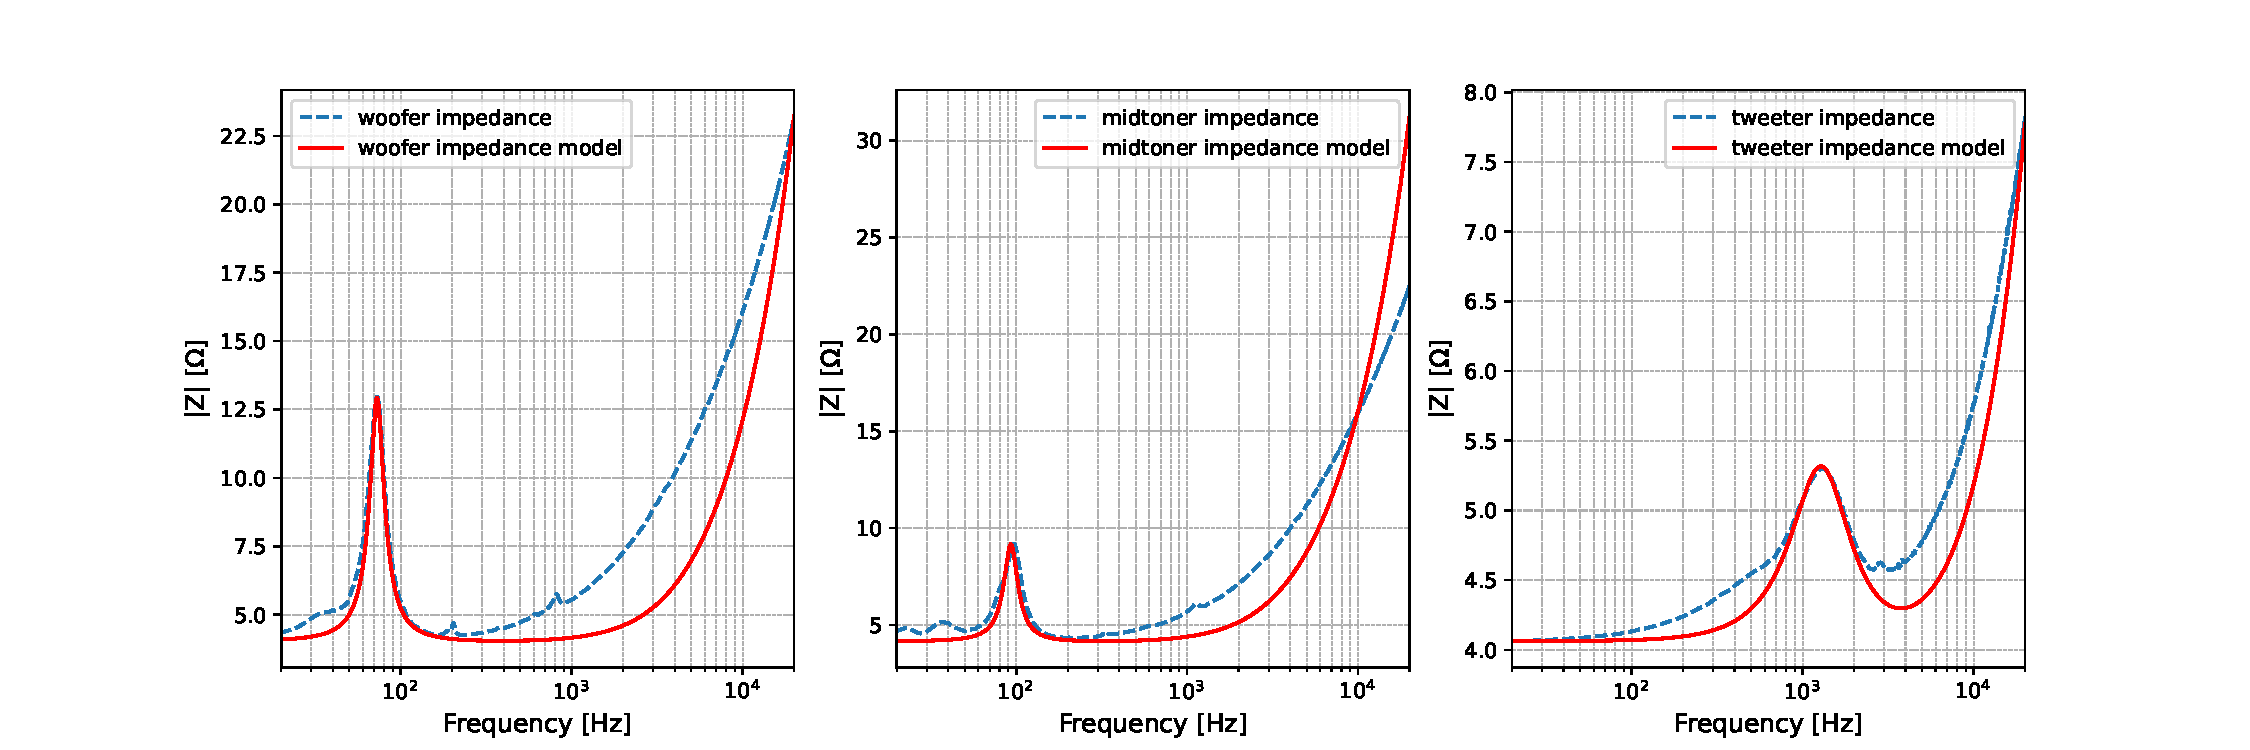
\includegraphics[width=1\textwidth]{TU Delft Booming Bass Project Report/figures/FilterGroup/model vs measured impedance.pdf}
    \captionsetup{justification=raggedright, labelfont=bf}
    \caption{Model speaker impedance versus measured speaker impedance}
    \label{fig:/model vs measured impedance}
\end{figure}

\section{Discussion}
Although the model matches the general shape of the impedance frequency behaviour of the physical circuit, there are still some discrepancies. The most significant of which is that the tweeter's model seems to be the least accurate of the three. This could probably be explained by the fact that the model is better suited for speakers with a lower resonant frequency. Also, at frequencies below and above the resonance peak, the model underestimates the impedance of all three speakers, most greatly for the tweeter.
However, the model does very accurately predict the impedance behavior of the speakers around their resonance peaks, which is the part where the speakers will do most of their work. So, it is most important that the model accurately describes these frequencies. 

\section{Conclusion}
The model of the speaker is an important of the design process as it allows simulations to be done using the model and thusly making the design process a lot simpler. Although the model doesn't match perfectly at every frequency, around the resonance peak it is quite accurate. 
%\chapter{Passive Filter Design}
\label{chapter:PassiveFilterDesign}

\section{Introduction}
A filter has to be effectively designed and built to block the unwanted frequencies to a specific speaker cone. This can prevent noise and damage to the cone. Therefore, it is vital to properly design the filters, which begs the question: 'In what manner can filters be effectively created to create the flattest acoustic response?'. A flat acoustic response means that the filters can reproduce the sound at all frequencies with the least change in volume. This would, therefore, help achieve the project's aim, which is to reproduce a sound with the highest accuracy possible. A flat acoustic response can help achieve this, as it will reproduce the sound with the least change in volume possible. Therefore, the filters must be designed to a high standard. This can be done by choosing the most optimal cut-off frequencies, evaluating the best order of the filter, deciding on a Zobel network or not, and selecting the best component values. 
\section{Specifications}
The specifications are that the frequency ranges from 20 to 20 kHz and that the audio is the most accurate possible. This, therefore, leaves the filter groups with a significant amount of flexibility in the design process of the filters. 

\section{Order of filter}
The initial requirement is choosing the order of the filter. This will be the base of the entire filter, as it decides what type of components the filter uses. The order of the filter changes the rate at which its amplitude responds around its cut-off frequencies. The transfer function of a first-order filter will decline by 20 decibels per decade, whereas a second-order filter's transfer function will decline by 40 decibels per decade. 

The significance of the greater decline is that the filter will act closer to an ideal filter, which would therefore make it fit closer to the models made for these filters. This is because, at the cut-off frequency, the filters' amplitude response will decrease to the half-power amplitude quicker with a steeper decline in the amplitude. At and after the half-power amplitude it can be approximated that the frequencies have a negligible impact on the speaker cone, as their power is not enough to make a significant contribution to amplify the sound. Therefore, it was reasoned that a second-order filter was in the best interest of the amplifier, as it would allow the filters to be bound more to the frequencies assigned to them, and have an insignificant impact outside this range. 

\section{Reasoning of Zobel network}
As seen in \ref{fig:/model vs measured impedance}, the impedance of the speaker increases at higher frequencies, which may therefore also cause a voltage increase over the loudspeaker. As a result, it can be said that the sound pressure in the speaker increases cite{IP-manual}. 

To prevent this from affecting the filters, there are two options. The first is taking into account the effect of the frequency-dependent impedance of the speaker. The other option is to connect a Zobel network in parallel with the filter. 

A Zobel network is a connection of elements in parallel with the speaker element so that the combined impedance is fully real. Consequently, the impedance of the speaker will be constant, and simplify calculations.

On the other hand, however, creating a Zobel network is a challenging task, as it requires simulating the network to find the optimal components. Once this is done there are the limitations of the components in the lab, making it unlikely that the Zobel network can fully remove the reactance of the loudspeaker. It may only decrease the frequency dependence of the impedance. Therefore, it was decided by the group that a Zobel network was not appropriate and therefore would not be used.  

\section{Calculation of cut-off frequencies}
Cut-off frequencies are where the transfer function has a gain of $\frac{\sqrt{2}}{2}$, which is considered the -3 dB frequency. For low-pass filters, after this point, frequencies will have a negligible effect on the output. Similarly, for high-pass filters, frequencies before the cut-off frequency have an insignificant impact. Moreover, for the band-pass filter, there are two cut-off frequencies, before the first and after the second, the frequencies are insignificant to the output. 

Deciding on the right cut-off frequencies is of high importance, as the aim of the project is to have the flattest acoustic response. Choosing the right cut-off frequencies plays a significant role in this, as it allows the frequency ranges for each of the speakers to be optimally chosen. Each speaker cone works optimally within a certain frequency range, where tweeters work in high frequencies, bass in low frequencies and mid-toners in between. Frequencies outside the optimal range can create low-quality sound or damage the cone. Therefore, it is important to choose the optimal cut-off frequencies. 

The best cut-off frequencies were chosen by overlaying the acoustic responses of each of the speakers in Python, as seen in \ref{fig: Cutoff frequencies}. Then by observation, and knowledge of the optimal frequency ranges of each of the cones, the cut-off frequencies were decided. This was done by finding where each of the speakers started to become unstable, and finding where the next speaker was stable enough to take over. With constructive and deconstructive interference between the sound waves, it would ultimately result in the flattest response possible.

The decided cut-off frequency for the low pass filter, as seen in fig\ref{fig: Cutoff frequencies} was 200 Hz. This was what we found would give us the flattest overall response. The cut-off frequency for the high-pass filter was 1250 Hz as it would give us a flat transition between the high-pass and band-pass filter. On the other hand, however, it can be noted that at 900 Hz in fig\ref{fig: Cutoff frequencies} there is a large dip in the power response of the mid-toner response. This dip has a significant impact on the overall response before the cut-off frequency. While we attempted to choose the most optimal cut-off frequencies, this dip is something we had to be cautious of. 
\begin{figure}[H]
    \centering
    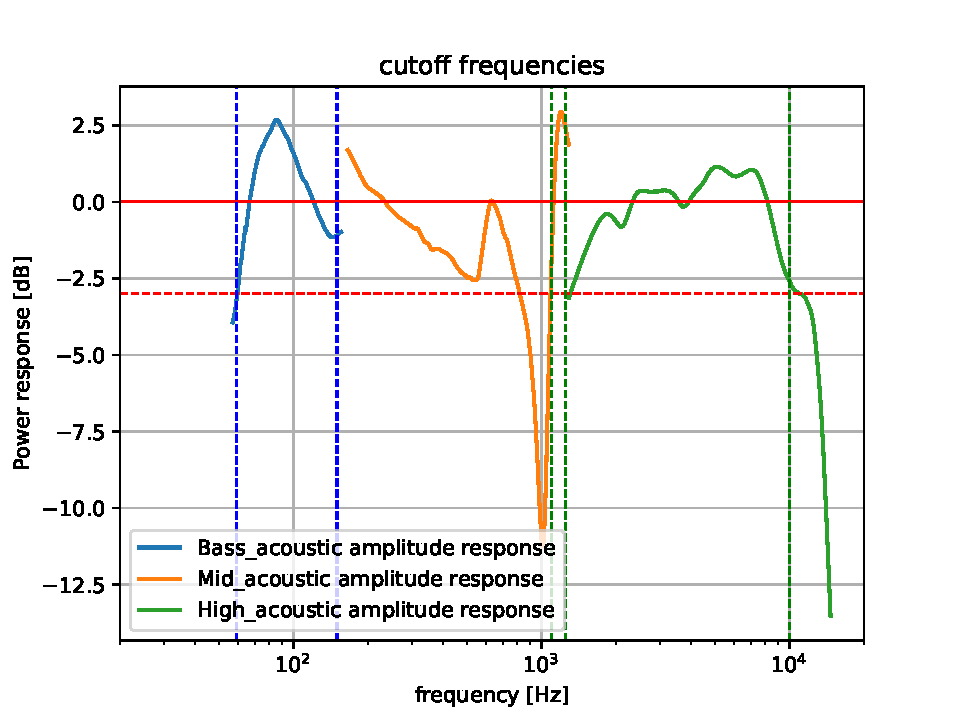
\includegraphics[width=0.6\linewidth]{TU Delft Booming Bass Project Report/figures/FilterGroup/chosenvalues.pdf}
    \captionsetup{justification=raggedright, labelfont=bf}
    \caption{Various amplitude responses plotted to assist in deciding initial cutt-off frequencies}
    \label{fig: Cutoff frequencies}
\end{figure}

\section{Transfer function}
Second-order passive filters are commonly described by their transfer functions, which express the relationship between the output voltage  out and the input voltage. This gives the following equation : 

According to the Kirchoff law 
V_in = V_R +V_L+V_C+V_out
\newline
Where here
\newline 
V_R (t) = R*I(t)  
\newline
V_L (t) = L* dI(t)/dt
\newline 
V_C = 1/c * integral (I(t))
\newline 
v_out = Zspk * I(t)
.




\section{Calculating component values}

\section{Simulations}

\section{Simulation results} %Dit is bode plots en de simulations 

 

\section{Discussion}

\section{Conclusions}

\subsection{Filter Requirements}
 Research question, specifications, reasoning of the required order, calculation
of the cutoff frequencies, reasoning if Zobel network required, transfer function, calculation of
required component values, simulations with nodal analysis, Bode diagrams including phase, discussion incl. comparison between theory, simulations and measurements, and conclusions.





%\chapter{Power Amplifier Design}
\label{chapter:PowerAmplifierDesign}




\section{Introduction}
Research question, specifications, reasoning of the employed topology,
derivation of the transfer function, nodal analysis simulations with LTSpice, and Bode diagrams including phase, measurement setup, measurement results, discussion including a comparison between theory, simulations and measurements, and conclusions.
%\chapter{Sound Amplifying System Acoustic Characterization}
\label{chapter:AcousticCharacterization}

\section{Introduction}
1- Algemene Inleiding (Wat gaan we maken, wat wil ik maken)
2- Achter grond
3- Uitbreiding over algemene requirments bijv kort requirments benoemen

\section{Methodology}

\section{Simulations}

\section{Measurments}

\section{Discussion}

\section{Conclusion}



%% Prevent urls running into margins in bibliography
\setcounter{biburlnumpenalty}{7000}
\setcounter{biburllcpenalty}{7000}
\setcounter{biburlucpenalty}{7000}

%% Add bibliography
\printbibliography[heading=bibintoc,title=Bibliography]

%% ----------------------------------------------------------------------
%%    Appendix (Letters for chapters)
%% ----------------------------------------------------------------------

\appendix

\chapter{Source Code}
\label{chapter: Code}


\section{Python Script - Ideal Filter Component Values Calculator}
\begin{lstlisting}[language=Python]
import numpy as np
from itertools import product

# Given cutoff frequencies
f_c1 = 150  # Hz for high-pass
f_c2 = 1250  # Hz for low-pass

# Component value lists
capacitor_values = [
    100e-9, 220e-9, 330e-9, 470e-9, 680e-9, 1e-6, 1.5e-6, 2.2e-6, 2.7e-6, 3.3e-6,
    3.9e-6, 4.7e-6, 5.6e-6, 6.8e-6, 8.2e-6, 10e-6, 15e-6, 22e-6, 33e-6, 47e-6, 100e-6
]

inductor_values = [
    0.15e-3, 0.22e-3, 0.33e-3, 0.47e-3, 0.68e-3, 1e-3, 1.5e-3, 2.2e-3, 3.3e-3, 4.7e-3
]

# Function to calculate cutoff frequency
def calculate_cutoff_frequency(L, C):
    return 1 / (2 * np.pi * np.sqrt(L * C))

# Perform a global search for the best values
best_high_pass = None
best_low_pass = None
best_error = float('inf')

for C_hp, L_hp, C_lp, L_lp in product(capacitor_values, inductor_values, capacitor_values, inductor_values):
    # Calculate cutoff frequencies for high-pass and low-pass
    f_c1_calc = calculate_cutoff_frequency(L_hp, C_hp)
    f_c2_calc = calculate_cutoff_frequency(L_lp, C_lp)

    # Compute the error as the sum of absolute differences
    error = abs(f_c1 - f_c1_calc) + abs(f_c2 - f_c2_calc)

    # Update best values if error is smaller
    if error < best_error:
        best_error = error
        best_high_pass = (C_hp, L_hp, f_c1_calc)
        best_low_pass = (C_lp, L_lp, f_c2_calc)

# Output the best results
print("High-pass filter:")
print(f"C_hp = {best_high_pass[0]:.2e} F, L_hp = {best_high_pass[1]:.2e} H, f_c1_actual = {best_high_pass[2]:.2f} Hz")
print("\nLow-pass filter:")
print(f"C_lp = {best_low_pass[0]:.2e} F, L_lp = {best_low_pass[1]:.2e} H, f_c2_actual = {best_low_pass[2]:.2f} Hz")
\end{lstlisting}
\section{Python Script -  BPF (Band-pass Filter) Frequency Response Graph}
\begin{lstlisting}[language=Python]
    import numpy as np
import scipy.signal as signal
import matplotlib.pyplot as plt

# Function to calculate Q, f0, and Bandwidth (BW) based on given fL and fH
def calculate_parameters(fL, fH):
    f0 = np.sqrt(fL * fH)  # Center frequency (f0)
    BW = fH - fL  # Bandwidth
    Q = f0 / BW  # Quality factor (Q)
    return f0, BW, Q

# Calculate LC components for a second-order low-pass filter
def calculate_LC_components_lowpass(f0, Q):
    L = Q / (2 * np.pi * f0)  # Inductor value in Henry
    C = 1 / (2 * np.pi * f0 * L)  # Capacitor value in Farad
    return L, C

# Calculate LC components for a second-order high-pass filter
def calculate_LC_components_highpass(f0, Q):
    C = Q / (2 * np.pi * f0)  # Capacitor value in Farad
    L = 1 / (2 * np.pi * f0 * C)  # Inductor value in Henry
    return L, C

# Function to design the second-order low-pass and high-pass filters (analog)
def design_filters(fL, fH, Q):
    # Analog low-pass filter transfer function
    omega_H = 2 * np.pi * fH  # Cutoff angular frequency for low-pass filter
    b_lp, a_lp = signal.butter(2, omega_H, btype='low', analog=True)  # Butterworth filter

    # Analog high-pass filter transfer function
    omega_L = 2 * np.pi * fL  # Cutoff angular frequency for high-pass filter
    b_hp, a_hp = signal.butter(2, omega_L, btype='high', analog=True)  # Butterworth filter

    return b_lp, a_lp, b_hp, a_hp

# Function to plot the combined frequency response of the bandpass filter
def plot_combined_response(b_lp, a_lp, b_hp, a_hp, fL, fH):
    # Create a frequency range for plotting (log scale)
    w, h_hp = signal.freqs(b_hp, a_hp, worN=np.logspace(1, 5, 400))  # Frequency response of HPF
    _, h_lp = signal.freqs(b_lp, a_lp, worN=w)  # Frequency response of LPF

    # Multiply the high-pass and low-pass responses to get the bandpass response
    h_bandpass = h_lp * h_hp

    # Plot the bandpass frequency response
    plt.figure(figsize=(10, 6))
    plt.semilogx(w, 20 * np.log10(np.abs(h_bandpass)), label='Bandpass Filter Response')
    plt.title(f"Bandpass Filter Frequency Response (fL={fL} Hz, fH={fH} Hz)")
    plt.xlabel('Frequency [Hz]')
    plt.ylabel('Magnitude [dB]')
    plt.grid(True)
    plt.legend()
    plt.show()

# Main function to design and plot the filter
def main(fL, fH):
    # Calculate f0, BW, and Q
    f0, BW, Q = calculate_parameters(fL, fH)

    # Print the calculated parameters
    print(f"Center frequency (f0): {f0:.2f} Hz")
    print(f"Bandwidth (BW): {BW:.2f} Hz")
    print(f"Quality factor (Q): {Q:.2f}")

    # Calculate the LC components for the low-pass filter
    L_lp, C_lp = calculate_LC_components_lowpass(f0, Q)
    print(f"Low-pass filter components:")
    print(f"Inductor (L) for low-pass filter: {L_lp:.6f} H")
    print(f"Capacitor (C) for low-pass filter: {C_lp:.6e} F")

    # Calculate the LC components for the high-pass filter
    L_hp, C_hp = calculate_LC_components_highpass(f0, Q)
    print(f"\nHigh-pass filter components:")
    print(f"Inductor (L) for high-pass filter: {L_hp:.6f} H")
    print(f"Capacitor (C) for high-pass filter: {C_hp:.6e} F")

    # Design the low-pass and high-pass filters
    b_lp, a_lp, b_hp, a_hp = design_filters(fL, fH, Q)

    # Plot the combined frequency response of the bandpass filter
    plot_combined_response(b_lp, a_lp, b_hp, a_hp, fL, fH)

# Example usage:
if __name__ == "__main__":
    fL = 150  # Low-pass cutoff frequency in Hz
    fH = 1250  # High-pass cutoff frequency in Hz
    main(fL, fH)

\end{lstlisting}


\section{Python - Phase Calculator}

\label{calculation of phase}
\begin{lstlisting}[language=Python]

def phase_calculation(frequency):
    f = frequency
    om = f * 2 * math.pi

    C_1 = 166.5 * (10 ** -9)
    R_2 = 47000
    C_a = 4.05 * (10 ** -9)
    R_a = 987
    R_b = 81800
    C_x = 968 * (10 ** -9)
    R_c = 1.98 * (10 ** 6)

    a = C_1 * R_2
    b = R_a * C_a
    d = a * b
    f = R_b * C_x
    k = (om ** 2) * a * R_c * C_x
    t = a+b+f
    q = (a*f) + k
    r = (f*(a+b)) + d
    
    Re_1 = ((om**4)*q*r) - ((om**2)*q)
    Re_2 = ((om**2)*a*t)-((om**4)*a*d*f)
    Re = Re_1 + Re_2

    Im_1 = (om*a) - ((om**3)*a*r)
    Im_2 = ((om**3)*q*t) - ((om**5)*d*f*q)
    Im = Im_1 + Im_2
    phase = np.degrees(np.atan(Im/Re))
    return phase

\end{lstlisting}
\newpage
\section{Python - Ripple and Average Voltage Simulations}
\label{sec:ripvoltcodesim}
\begin{lstlisting}[language=Python]
import pandas as pd

def ripple(avg, max):
    return (max-avg)/avg*100


datas = [(".\\19 ohm.txt",19),
    	(".\\38 ohm.txt",38),
    	(".\\76 ohm.txt",76),
    	(".\\no load.txt",None)]

for data in datas:
    file = data[0]
    resistance = data[1]
    
    data = pd.read_csv(file, delimiter="\t")
    #Only take the last part of the simulation to avoid the waveform when the capacitors are still being loaded
    t = data["time"][len(data["time"])//3*2:]
    v = data["V(n001)"][len(data["V(n001)"])//3*2:]
    i = data["I(R2)"][len(data["I(R2)"])//3*2:]

    maxV = v.max()
    minV = v.min()
    avgV = (maxV + minV)/2
    meanI = i.mean()
    
    if resistance == None:
        print(f"Using {file} (Power supply is not loaded)")
    else:
        print(f"Using {file} (Power supply is loaded with a {resistance} Ohm resistor)")

    print(f"    Load resistance: {resistance}")   
    print(f"    Average Voltage: {avgV:.3}V")
    print(f"    Average Current: {meanI:.3}A")
    print(f"    Ripple: {ripple(avgV, maxV):.3}%")
\end{lstlisting}

\section{Python - Ripple and Average Voltage Measurements}
\label{sec:ripvoltcodemea}

\begin{lstlisting}[language=Python]
import pandas as pd

def ripple(avg, max):
    return (max-avg)/avg*100
# Tuples are formatted as (filename,resistance)
datas = [(".\\19 ohm\\F0009CH1.CSV",19),
    	(".\\38 ohm\\F0007CH1.CSV",38),
    	(".\\76 ohm\\F0011CH1.CSV",76),
    	(".\\No load\\F0008CH1.CSV",None)]
for data in datas:
    file = data[0]
    resistance = data[1]
    
    measured_data = pd.read_csv(file, usecols=[3,4])
    t = measured_data["d"]
    v = measured_data["e"]

    maxV = v.max()
    minV = v.min()
    avgV = (maxV + minV)/2
    if resistance == None:
        print(f"Using {file} (Power supply is not loaded)")
    else:
        print(f"Using {file} (Power supply is loaded with a {resistance} Ohm resistor)")
    print(f"    Load resistance: {resistance}")   
    print(f"    Average Voltage: {avgV:.3}V")
    if resistance == None:
        print(f"    Average Current: 0.00A")
    else:
        print(f"    Average Current: {avgV/resistance:.3}A")
    print(f"    Ripple: {ripple(avgV, maxV):.3}%")

\end{lstlisting}


\DeclareTCBListing{mintedbox}{O{}m!O{}}{%
  breakable=true,
  listing engine=minted,
  listing only,
  minted language=#2,
  minted style=default,
  minted options={%
    linenos,
    gobble=0,
    breaklines=true,
    breakafter=,,
    fontsize=\small,
    numbersep=8pt,
    #1},
  boxsep=0pt,
  left skip=0pt,
  right skip=0pt,
  left=25pt,
  right=0pt,
  top=3pt,
  bottom=3pt,
  arc=5pt,
  leftrule=0pt,
  rightrule=0pt,
  bottomrule=2pt,
  toprule=2pt,
  colback=bg,
  colframe=orange!70,
  enhanced,
  overlay={%
    \begin{tcbclipinterior}[h!]
    \fill[orange!20!white] (frame.south west) rectangle ([xshift=20pt]frame.north west);
    \end{tcbclipinterior}},
  #3}

\chapter{Power Supply Appendix}
%\label{chapter:title}

\section{Intermediate Report Power Supply}
\href{https://github.com/Miyanooooo/FinalReport.git}{B2-1 and B2-2's Power Supply Intermediate Reports (external link)}


%\chapter{Filter Appendix}

\chapter{Power Amplifier Appendix}



\captionsetup{justification=centering, labelfont=bf}


\subsection{Non-Ideal Op-Amp}
\begin{figure}[H]
    \centering
    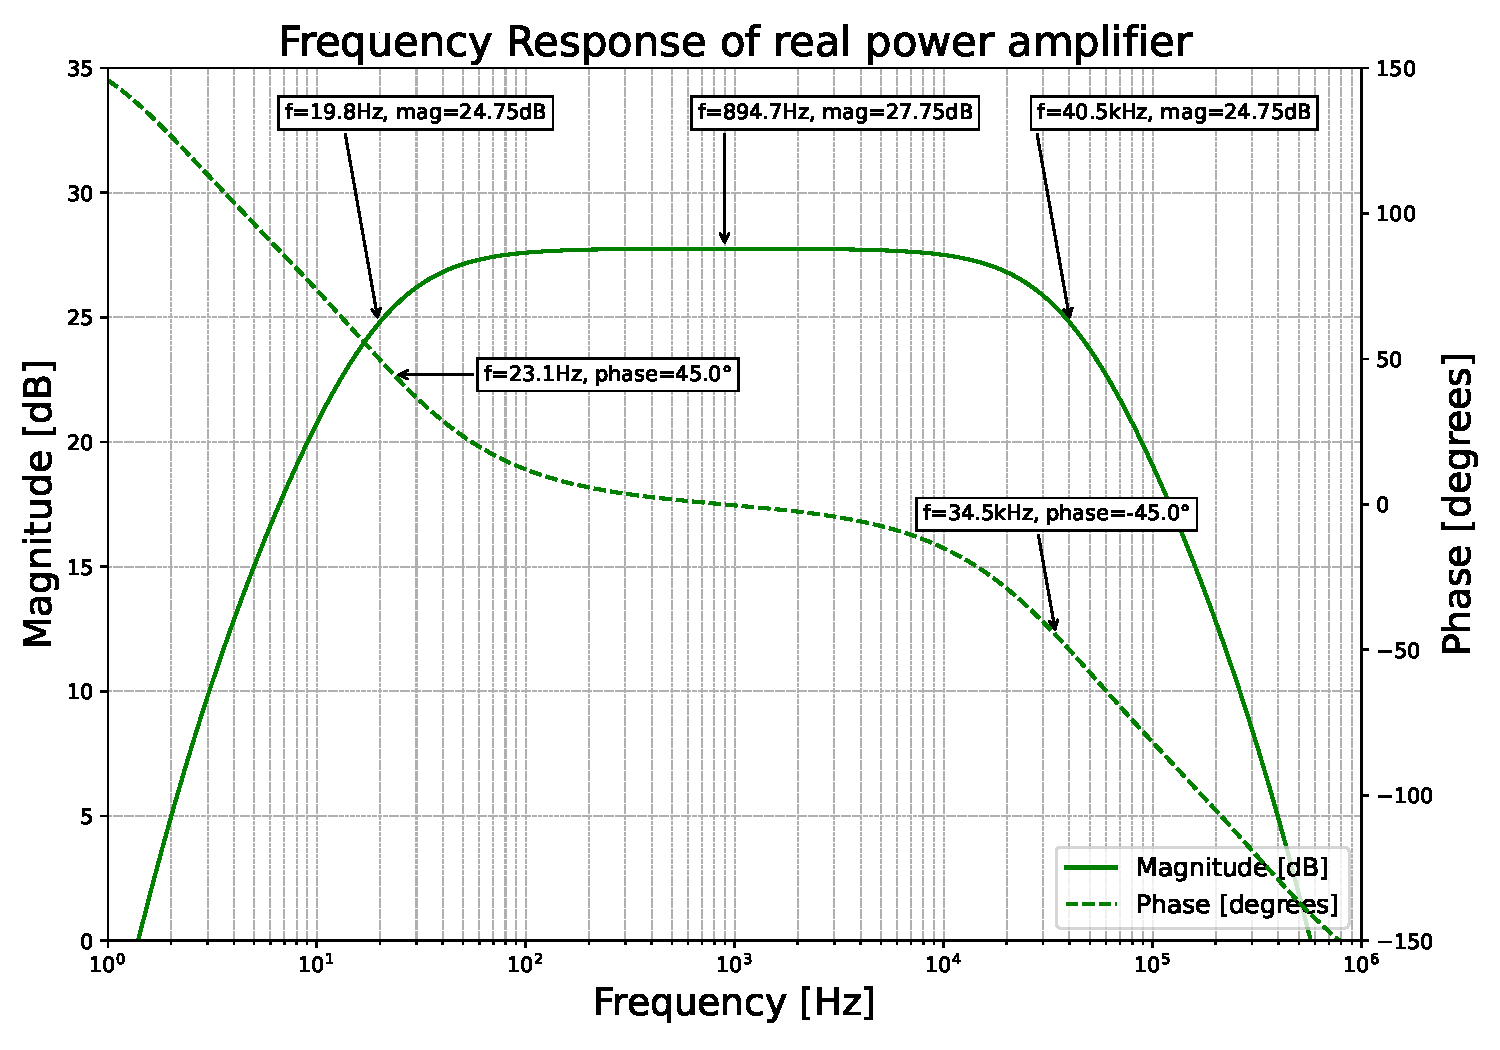
\includegraphics[width=0.9\linewidth]{TU Delft Booming Bass Project Report/figures/PowerAmplifier/not ideal amplifier results.pdf}
    \captionsetup{justification=raggedright, labelfont=bf}
    \caption{The results of the power amplifier circuit, using what were considered to be the ideal component values, are shown.}
    \label{fig:not ideal amplifier}
\end{figure}
\newpage
\subsection{Calculation of $\mathbf{R_c}$}
\label{calculation of Rc}
The circuit diagram used to calculate $R_c$ is shown in Fig. \ref{fig: non ideal active high}:

\begin{figure}[H]
    \centering
    \begin{minipage}[T]{0.55\textwidth}
        \centering
        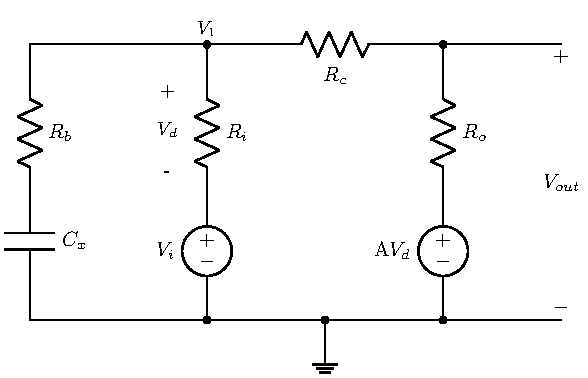
\includegraphics[width=\linewidth]{TU Delft Booming Bass Project Report/figures/PowerAmplifier/circuits/non_ideal opamp circuit.pdf}
        \captionsetup{justification=raggedright, labelfont=bf}
        \caption{The non-ideal equivalent circuit to \autoref{fig: pa active high pass}.}
        \label{fig: non ideal active high}
    \end{minipage}%
    \hspace{0.05\textwidth} % Adjust space between figure and table
    \begin{minipage}[T]{0.35\textwidth}
        \centering
        \begin{tabular*}{0.9\textwidth}{@{\extracolsep{\fill}} c c @{}}
            \toprule
            \textbf{Component} & \textbf{Value of Component} \\
            \midrule
            \textbf{$C_x$} & 79.5$\mu$F \\
            \textbf{$R_b$} & 1k$\Omega$ \\ 
            \textbf{$R_i$} & 200k$\Omega$ \\
            \textbf{$R_o$} & 10$\Omega$ \\
            A & $10^5$ \\
            \bottomrule
        \end{tabular*}
        \captionsetup{justification=raggedright, labelfont=bf}
        \caption{Component values in the non-ideal circuit.}
        \label{tab:ideal values}
    \end{minipage}
\end{figure}







From the circuit, it is clear that the following holds:
\begin{flalign*}
    V_o = 25V_i, \quad V_d = V_1 - V_i
\end{flalign*}
Applying nodal analysis at node $V_1$ in circuit of Fig. \ref{fig: non ideal active high}, gives:
\begin{flalign*}
    \frac{V_{o}-V_{1}}{R_C} + \frac{V_o- 10^5(V_1-V_i)}{R_o} =0 \\
    10(25V_i - V_1) + R_c\left(25V_i - 10^5(V_1 - V_i)\right) = 0 \\
     R_c = -\frac{10(25V_i-V_1)}{25V_i - 10^5V_1 + 10^5V_i} \\
\end{flalign*}

\begin{flalign}
    25V_i + 10^5V_i \approx 10^5 V_i
\end{flalign}

\begin{flalign}
\label{eq: 1}
    R_c = -\frac{25 V_i - V_1}{10^4(V_i-V_1)}
    \equnit{\si{\Omega}}
\end{flalign}


Applying nodal analysis at node 2 gives:
\[\frac{V_1}{R_b + Z_c} + \frac{V_1-V_i}{R_i} + \frac{V_1-V_o}{Rc} = 0\]
\[\frac{V_1 R_c}{R_b + Z_c} + \frac{(V_1-V_i)R_c}{R_i} + {V_1-V_o} = 0\]

\[R_c\left(\frac{V_1}{R_b + Z_c} + \frac{V_1-V_i}{R_i}\right) =  25V_i-V_1\]

\begin{equation}
\label{eq: 2}
    Rc = \frac{25V_i-V_1}{\frac{V_1}{R_b + Z_c} + \frac{V_1-V_i}{R_i}}
\end{equation}

By comparing Eq. (\ref{eq: 1}) and (\ref{eq: 2}), follows that:
\[ -\frac{25 V_i - V_1}{10^4V_i - 10^4 V_1} = \frac{25V_i-V_1}{\frac{V_1}{R_b + Z_c} + \frac{V_1-V_i}{R_i}}\]
\[10^4(V_1-V_i) = \frac{V_1}{R_b + Z_c} + \frac{V_1-V_i}{R_i}\]

\[\left(\frac{1}{R_b + Z_c} + \frac{1}{R_i}-10^4\right)V_1 = \left(\frac{1}{R_i}-10^4\right)V_i\] 
For $R_i=200\text{k}\Omega$, gives: 
\[\frac{1}{R_i} -10^4 \Rightarrow \frac{1}{200k} - 10^4 \approx -10^4\]
\begin{flalign}
\label{eq: 3}
    V_1 = \left(\frac{-10^4}{\frac{1}{R_b + Z_c}-10^4}\right)Vi = aV_i
\end{flalign}
where $a = 1-7.95\cdot10^{-16} j\omega$. Substituting Eq. (\ref{eq: 3}) in (\ref{eq: 1}), gives that:
\begin{flalign*}
    R_c = \frac{a-25}{10^4(a-1)}\left(\frac{V_i}{V_i}\right)
    \equnit{\si{\Omega}}
\end{flalign*}

Putting these values in a calculator gives that $R_c$:
\begin{flalign*}
    R_c= (2.4\cdot10^{4}) - 1.9j\omega\cdot10^{-3}\Omega
    \equnit{\si{\Omega}}
\end{flalign*}

The real part is approximately an order of 7 greater than the imaginary part, making the imaginary component negligible until frequencies well beyond the circuit's requirements and operation conditions, resulting in:
\begin{flalign*}
    R_c \approx 24k\Omega \Rightarrow R_c= 24R_b
\end{flalign*}







\subsection{Total Transfer Function Derivation}
\label{total transfer}

To obtain the total transfer function, the functions \ref{eq: E}, \ref{eq: F} and \ref{eq: G} must be multiplied together. This can be done as follows:


\begin{flalign*}
    \mathbf{E(\omega)} = \frac{R_2 C_1 s}{s R_1 C_1 + 1}, \quad \mathbf{F(\omega)} = \frac{1}{s R_a C_a + 1}, \quad \mathbf{G(\omega)} = \frac{R_C}{R_b + \frac{1}{s C_x}}+1
\end{flalign*}

Let $a = R_2 C_1$, $b = R_a C_a$, $d =ab$, $f = R_b C_x$, and $k = R_2 C_1 R_c C_x$:
\begin{flalign*}
    \frac{sa}{s a + 1}\left(\frac{1}{s b + 1}\right) = \frac{sa }{(s a + 1)(s b + 1)}
\end{flalign*}
\begin{flalign*}
    \mathbf{H(\omega)} = \frac{sa}{s^2 d + s a + s b + 1}=\frac{sa}{e}
\end{flalign*}
where $e = s^2 d + s a + s b  + 1$, gives:
\begin{flalign*}
    \frac{sa }{e}\left(\frac{R_C}{R_b + \frac{1}{s C_x}}+1 \right) = \frac{sa }{e}\left( \frac{s R_C C_x}{s R_b C_x  + 1}+1 \right)
\end{flalign*}






\[
\frac{s a}{e} + \frac{s^2 k}{e(sR_b C_x+1)} = \frac{s a (sf + 1) + s^2 k}{e \big(sf + 1 \big)}
\]

\[\frac{s^2( af+ k) + s a }{e \big(sf + 1 \big)}\]

Substituting all of the variables given earlier, gives:
\begin{flalign*}
    \mathbf{H(\omega)} = \frac{s^2 R_2 C_1 R_b C_x + s^2 R_2 C_1 R_c C_x+ s R_2 C_1 }{(s^2 C_1 C_a R_2 R_a + sC_a R_a + sC_1 R_2+1)(R_b C_x s + 1 )}
\end{flalign*}
\begin{flalign}\label{eq: third order}
    e(sf+1) &= (s^2 d+ s(a+b) +1)(sf + 1 ) \notag\\
            &= s^3df + s^2f(a+b) +sf + s^2d + s(a+b) + 1 \notag\\
            &= s^3df + s^2(f(a+b) + d) + s(a+b+f) + 1
\end{flalign}

Thus giving:
\begin{flalign*}
    \mathbf{H(\omega)} = \frac{s^2( af+ k) + s a }{s^3df + s^2(f(a+b) + d) + s(a+b+f) + 1}
\end{flalign*}
Let $t = a+b+f$, $q = af + k$, and $r = f(a+b) + d$:

%( \[\frac{\frac{1}{s^2}}{\frac{1}{s^2}} \cdot H(\omega) = \frac{R_2 C_1 R_b C_x + R_c R_2 C_1 C_x+  \frac{R_2 C_1}{s} }{sdf + f(a+b) + d + \frac{1}{s}(a+b+f) + \frac{1}{s^2}}\])\\
This gives: 
\begin{flalign}
\mathbf{H(\omega)} &= \frac{s^2q+ s a }{ (s^2r + 1) + s(s^2df + t)}
\end{flalign}
\subsubsection{Derivation for Phase Formula}
\label{sec: phase calc}
To calculate the phase, $\mathbf{H(\omega)}$ must be multiplied by its complex conjugate. After separating the real and imaginary parts of the enumerator, the expression becomes:
\begin{flalign*}
    \mathbf{H(\omega)} &= \frac{s^2q+ s a }{ (s^2r + 1) + s(s^2df + t)}\left(\frac{(s^2r + 1) - s(s^2df + t)}{(s^2r + 1) - s(s^2df + t)}\right)\\
                        &= \frac{(s^2q + s a)((s^2r + 1) - s(s^2df + t)) }{ (s^2r + 1)^2 - s^2(s^2df + t)^2}
\end{flalign*}
\begin{flalign*}
    h = (s^2r + 1)^2 - s^2(s^2df + t)^2
\end{flalign*}

Multiplying the denominator by the first part of the conjugate results in:
\begin{flalign*}
    &= (s^2q+ s a)(s^2r + 1) \\
    &=s^4qr +  s^3ar +s^2q + sa
\end{flalign*}
And thus giving for its real and imaginary part:
\begin{flalign*}
    \text{Re}_1= \frac{\omega^4qr - \omega^2q}{h} \\
    \text{Im}_1 = \frac{\omega a-\omega^3ar}{h}
\end{flalign*}

Multiplying the denominator by the second part of the conjugate results in:
\begin{flalign*}
    (s^2q+ s a)(-s(s^2df + t) ) &= -s(s^2q+ s a)(s^2df + t ) \\
                                &=-s^5dfq - s^3qt - s^2at - s^4adf
\end{flalign*}

Thus resulting in: 
\begin{flalign*}
    \text{Re}_2 = \frac{\omega^2at-\omega^4adf}{h} \\
    \text{Im}_2 = \frac{\omega^3qt-\omega^5dfq}{h}
\end{flalign*}

For the total real and imaginary part, the following holds:
\begin{flalign*}
    \text{Re} = \text{Re}_1 + \text{Re}_2 \notag\\
    \text{Im} = \text{Im}_1 + \text{Im}_2 \notag\\
    \phi_{\text{Phase}} = \arctan\left(\frac{\text{Im}}{\text{Re}}\right)
\end{flalign*}







\newpage




\DeclareTCBListing{mintedbox}{O{}m!O{}}{%
  breakable=true,
  listing engine=minted,
  listing only,
  minted language=#2,
  minted style=default,
  minted options={%
    linenos,
    gobble=0,
    breaklines=true,
    breakafter=,,
    fontsize=\small,
    numbersep=8pt,
    #1},
  boxsep=0pt,
  left skip=0pt,
  right skip=0pt,
  left=25pt,
  right=0pt,
  top=3pt,
  bottom=3pt,
  arc=5pt,
  leftrule=0pt,
  rightrule=0pt,
  bottomrule=2pt,
  toprule=2pt,
  colback=bg,
  colframe=orange!70,
  enhanced,
  overlay={%
    \begin{tcbclipinterior}[h!]
    \fill[orange!20!white] (frame.south west) rectangle ([xshift=20pt]frame.north west);
    \end{tcbclipinterior}},
  #3}


%\chapter{Task Division}
%\label{chapter:title}


\begin{table}[htb]
    \setlength\extrarowheight{4pt}
    \centering
    \caption{Distribution of the workload}
    \label{tab:taskdivision}
    \begin{tabularx}{\textwidth}{lXX}
        \toprule
        & Task & Student Name(s) \\
        \midrule
        & Summary & \\
        Chapter 1 & Power Supply Analysis & A. Guo \& G.D. van Weelden \\
        Chapter 2 & Loudspeaker Analysis & \\
        Chapter 3 & Passive Filter Design & \\
        Chapter 4 & Power Amplifier Design & \\
        Chapter 6 & Sound Amplifying System Acoustic Characterization & \\
        Chapter 7 & Conclusion &  \\
        \midrule
        & Editors & \\
        & CAD and Figures & \\
        & Document Design and Layout & A. Guo \\
        \bottomrule
    \end{tabularx}
\end{table}



\end{document}
